%%%%%%%%%%%%%%%%%%%%%%%%%%%%%%%%%%%%%%%%%%%%%%%%%%%%%%%%%%%%%%%%%%%%%%
% Lớp 11 | Quan hệ vuông góc trong không gian | Hình lăng trụ đứng. Hình chóp đều. Thể tích
% Dạng 1H8?7-3: Thể tích khối chóp tứ giác
% Số câu: 81  (sinh tự động bởi tach_cau.py; từ nay thầy sửa trực tiếp file này)
%%%%%%%%%%%%%%%%%%%%%%%%%%%%%%%%%%%%%%%%%%%%%%%%%%%%%%%%%%%%%%%%%%%%%%

%%%%%%%%%%%%%%%% TRẮC NGHIỆM 4 PHƯƠNG ÁN %%%%%%%%%%%%%%%%

% nguồn: Ok_TracNghiemLop11_Lan1
\begin{ex}%[1H8N7-3]%[ma:0f2d0a7b]
	Cho khối chóp tứ giác đều có  cạnh đáy bằng $a \sqrt{2}$, chiều cao bằng $a$. Thể tích $V$ của khối chóp đó là
	 \choice
		{\True $V=\dfrac{2 a^3}{3}$} 
		{$V=\dfrac{a^3 \sqrt{2}}{3}$} 
		{$V=2 a^3$} 
		 {$V=\dfrac{a^3 \sqrt{7}}{3}$}
	 \loigiai{
	Khối chóp tứ giác đều nên đáy là hình vuông có diện tích  là $S=(a \sqrt{2})^2=2 a^2$.\\
	Thể tích $V$ của khối chóp đó là $V=\dfrac{1}{3} S \cdot  h=\dfrac{1}{3} \cdot 2 a^2 \cdot a=\dfrac{2 a^3}{3}$.
	} 
\end{ex}

% nguồn: Ok_Toan11_TracNghiem_Lan2
\begin{ex}%[1H8H7-3]%[ma:3809e2eb]
	Cho hình hộp đứng có cạnh bên có độ dài là $3a$, đáy  là hìn thoi cạnh $a$ và có một góc bằng $60^{\circ}$. Thể tích khối hộp đã cho là
	 \choice
		 {$\dfrac{3a^3\sqrt{3}}{4}$}
		{$\dfrac{a^3\sqrt{3}}{3}$} 
		 {$\dfrac{a^3\sqrt{3}}{2}$}
		{\True $\dfrac{3a^3\sqrt{3}}{2}$} 
	\loigiai{ 
	\immini{ 
		Xét $\triangle{ABC}$ cân tại $B$ có $\widehat{B}=60^{\circ}$. 
		Suy ra  $\triangle{ABC}$ đều.\\
		Suy ra  $S_{ABCD}=2S_{\triangle{ABC}}=2\cdot\dfrac{a^2\sqrt{3}}{4}=\dfrac{a^2\sqrt{3}}{2}$.\\
		 Thể tích khối hộp đã cho là $$V_{ABCD.A'B'C'D'}=S_{ABCD}\cdot A'A=\dfrac{a^2\sqrt{3}}{2}\cdot 3a=\dfrac{3a^3\sqrt{3}}{2}.$$
		}{ 
		\begin{tikzpicture}[scale=1,font=\footnotesize,line join=round,line cap=round,>=stealth]
				\def\bc{4} 
				\def\ba{2} 
				 \def\h{3}
				\def\gocB{30} 
				\coordinate (B) at  (0,0);
				\coordinate (A)  at (\gocB:\ba);
				\coordinate (C)  at (\bc,0);
				\coordinate  (D) at ($(C)-(B)+(A)$);
				 \coordinate (A') at ($(A)+(90:\h)$);
				\coordinate (B') at ($(B)-(A)+(A')$); 
				\coordinate (C') at ($(C)-(A)+(A')$); 
				 \coordinate (D') at ($(D)-(A)+(A')$);
				\draw  (B')--(B)--(C)--(D)--(D')--(A')--(B')--(C')--(D')
					 (C)--(C');
				\draw[dashed] (A')-- node [right]{$3a$} 
					(A)--(D) 
					 (C)--(A)--(B);
				\foreach \x/\g  in {A/-90,B/-90,C/-90,D/-90,A'/90,B'/90,C'/90,D'/90}
				\fill (\x)  circle (1pt)+(\g:3mm) node {$\x$};
				 \draw pic["$60^\circ$",draw,angle eccentricity=1.4,angle radius=0.8cm]{angle=C--B--A};
			\end{tikzpicture}
		 }
	 }
\end{ex}

% nguồn: Ok_Toan11_TracNghiem_Lan2
\begin{ex}%[1H8H7-3]%[ma:0a29f46b]
	Cho hình chóp tứ giác $S.ABCD$ có đáy $ABCD$ là  hình vuông cạnh $a$, mặt bên $SAB$ là tam giác đều và nằm trong mặt phẳng vuông góc với đáy $(ABCD)$. Tính thể tích khối chóp $S.ABCD$.
	\choice 
		 {$\dfrac{a^3}{6}$}
		{\True $\dfrac{a^3\sqrt{3}}{6}$} 
		{$\dfrac{a^3\sqrt{3}}{2}$} 
		{$10$} 
	 \loigiai{
	 \immini{
		Gọi $H$ là trung điểm $AB$ thì $SH\perp  AB$ và $SH=\dfrac{a\sqrt{3}}{2}$.\\
		Ta có $\heva{&(SAB)\perp (ABCD) \\&(SAB)\cap (ABCD)=AB \\&SH\perp AB}\Rightarrow SH\perp (ABCD)$.\\ 
		Diện tích đáy $S_{ABCD}=AB^2=a^2$.\\ 
		Vậy thể tích khối chóp $S.ABCD$ là $$V_{S.ABCD}=\dfrac{1}{3}SH\cdot  S_{ABCD}=\dfrac{a^3\sqrt{3}}{6}.$$
		 }{
		\begin{tikzpicture}[scale=0.7,>=stealth,line join=round,line cap=round,font=\footnotesize]
				 \def\a{4}
				 \def\h{4}
				\def\r{2} 
				\def\al{-145} 
				\path 
					(0,0) coordinate (A) 
					 (\al:\r) coordinate (B)
					(\a,0) coordinate (D) 
					($(B)+(D)-(A)$) coordinate  (C)
					 ($(B)!1/2!(A)$) coordinate (H)
					($(H)+(0,\h)$) coordinate (S); 
				\draw (S)--(B)--(C)--(S)--(D)--(C); 
				\draw[dashed,thin]  (B)--(A)--(S)
					 (A)--(D)
					 (S)--(H);
				\foreach \p/\g  in {A/160,B/-120,C/-45,D/0,S/90,H/160}\fill (\p) circle (1pt) node[shift={(\g:.3)}]{$\p$};
				\foreach  \a/\b/\c in {S/H/A}
					{\draw pic[draw,angle  radius=2mm] {right angle = \a--\b--\c};};
			\end{tikzpicture}
		 }
	} 
\end{ex}

% nguồn: Ok_Toan11_TracNghiem_Lan2
\begin{ex}%[1H8H7-3]%[ma:981e91ff]
	 Cho hình lăng trụ đứng $ABCD.A'B'C'D'$ có đáy là hình thoi. Biết $A'A=4a$, $AC=2a$ và $BD=a$. Thể tích của khối lăng trụ đã cho là
	 \choice
		{$8a^3$} 
		 {$2a^3$}
		 {$\dfrac{8}{3}a^3$}
		{\True $4a^3$} 
	\loigiai{ 
	 \immini{
		Diện tích hình thoi  $ABCD$ là $S_{ABCD}=\dfrac{1}{2}\cdot AC\cdot BD=\dfrac{1}{2}\cdot2a\cdot a=a^2$.\\
		Thể tích khối  lăng trụ đã cho là $V=S_{ABCD}\cdot A'A=a^2\cdot4a=4a^3$.
		 }{
		\begin{tikzpicture}[scale=1,font=\footnotesize,line join=round,line cap=round,>=stealth]
				 \def\bc{4}
				\def\ba{2} 
				\def\h{3} 
				 \def\gocB{30}
				\coordinate (B) at  (0,0);
				\coordinate (A) at  (\gocB:\ba);
				 \coordinate (C) at (\bc,0);
				\coordinate (D) at ($(C)-(B)+(A)$); 
				\coordinate (A') at  ($(A)+(90:\h)$);
				\coordinate  (B') at ($(B)-(A)+(A')$);
				\coordinate (C')  at ($(C)-(A)+(A')$);
				\coordinate (D')  at ($(D)-(A)+(A')$);
				 \draw (B')--(B)--(C)--(D)--(D')--(A')--(B')--(C')--(D')
					 (C)--(C');
				\draw[dashed] (A')-- node [right]{$4a$} 
					 (A)--(D)
					(A)--(B); 
				\foreach \x/\g in  {A/-90,B/-90,C/-90,D/-90,A'/90,B'/90,C'/90,D'/90}
				\fill (\x) circle (1pt)+(\g:3mm) node {$\x$}; 
			\end{tikzpicture}
		 }
	} 
\end{ex}

% nguồn: Ok_Toan11_TracNghiem_Lan2
\begin{ex}%[1H8H7-3]%[ma:69b3f058]
	Cho khối chóp tứ giác đều có cạnh đáy bằng $a$, cạnh bên gấp hai lần cạnh đáy. Tính thể  tích $V$ của khối chóp đã cho.
	 \choice
		 {\True $V=\dfrac{\sqrt{14}a^3}{6}$}
		{$V=\dfrac{\sqrt{14}a^3}{2}$} 
		{$V=\dfrac{\sqrt{2}a^3}{2}$} 
		 {$V=\dfrac{\sqrt{2}a^3}{6}$}
	\loigiai{ 
	 \immini{
		Gọi $O$  là tâm hình vuông $ABCD$, ta có $SO\perp (ABCD)$.\\
		 Trong tam giác $SOC$ vuông tại $O$, $SO=\sqrt{SC^2-OC^2}=\dfrac{a\sqrt{14}}{2}$.\\
		Vậy $V=\dfrac{1}{3} SO\cdot{S_{ABCD}}=\dfrac{1}{3}\cdot  \dfrac{a\sqrt{14}}{2}\cdot a^2=\dfrac{a^3\sqrt{14}}{6}$.
		}{ 
		\begin{tikzpicture}[scale=0.8,>=stealth,line join=round,line cap=round,font=\footnotesize]
				\def\a{4} 
				\def\h{4} 
				 \def\r{2}
				 \def\al{-145}
				 \path
					(0,0) coordinate  (A)
					(\al:\r) coordinate (B) 
					(\a,0) coordinate (D) 
					 ($(B)+(D)-(A)$) coordinate (C)
					($(A)!1/2!(C)$) coordinate (O) 
					($(O)+(0,\h)$) coordinate (S); 
				\draw  (S)--(B)--(C)--(S)--(D)--(C);
				\draw[dashed,thin] (B)--(A)--(S)--(O) 
					(C)--(A)--(D)--(B); 
				 \foreach \p/\g in {A/160,B/-120,C/-45,D/0,S/90,O/-90}\fill (\p) circle (1pt) node[shift={(\g:.3)}]{$\p$};
				 \foreach \a/\b/\c in {S/O/A}
					{\draw pic[draw,angle radius=2mm] {right angle  = \a--\b--\c};};
			\end{tikzpicture}
		 }
	 }
\end{ex}

% nguồn: Ok_Toan11_TracNghiem_Lan2
\begin{ex}%[1H8H7-3]%[ma:186a2412]
	Cho hình chóp tứ  giác đều có cạnh đáy bằng $a$, góc giữa cạnh bên và mặt đáy bằng $60^\circ$. Thể tích khối chóp là
	 \choice
		 {\True $\dfrac{a^3\sqrt{6}}{6}$}
		{$\dfrac{a^3\sqrt{6}}{2}$} 
		 {$\dfrac{a^3\sqrt{3}}{6}$}
		{$\dfrac{a^3\sqrt{6}}{3}$} 
	\loigiai{ 
	\immini 
		{ 
		 Giả sử hình chóp tứ giác đều là $S.ABCD$.\\
		Gọi $O$  là giao điểm của $BD$ và $AC$.\\
		Ta có $SO\perp(ABCD)$, $\widehat{SAO}=60^\circ$,  $AC=a\sqrt{2}\Rightarrow OA=\dfrac{a\sqrt{2}}{2}$.\\
		Khi đó $SO=AO\cdot\tan\widehat{SAO}=\dfrac{a\sqrt{6}}{2}$,  $S_{ABCD}=a^2$.\\
		Thể tích khối chóp là  $V=\dfrac{1}{3}SO\cdot S_{ABCD}=\dfrac{a^3\sqrt{6}}{6}$.
		} 
		{ 
		\begin{tikzpicture}[=>stealth,line join=round,line cap=round,font=\footnotesize,scale=.6]
				\def\a{5} 
				 \def\goc{210}
				\def\b{3} 
				 \def\h{4.5}
				 \path
					(0,0) coordinate (A)++(0:\a) coordinate  (B)++(\goc:\b) coordinate (C)++(180:\a) coordinate (D)
					 ($(A)!.5!(C)$) coordinate (O)
					(O)++(90:\h) coordinate  (S);
				\draw (S)--(B)--(C)--(D)--cycle (S)--(C); 
				 \draw[dashed] (O)--(S)--(A)--(C)
					(B)--(A)--(D) 
					 (B)--(D);
				\foreach  \x/\g in{A/160,B/0,C/-90,S/90,O/-90,D/-90}
				 \fill(\x) circle (1pt)
					($(\x)+(\g:3mm)$)  node{$\x$};
				 \draw pic[draw,angle radius=1mm] {right angle = S--O--C};
				\pic[draw,angle radius=2mm,angle eccentricity=1.79]  {angle = O--A--S};
			\end{tikzpicture}
		} 
	 }
\end{ex}

% nguồn: Ok_Toan11_TracNghiem_Lan2
\begin{ex}%[1H8H7-3]%[ma:7576e9f2]
	Cho hình chóp $S.ABCD$ có đáy $ABCD$ hình chữ nhật với $AB=4a, BC=a$, cạnh bên $SD=2a$ và $SD$ vuông góc với mặt phẳng đáy.  Thể tích khối chóp $S.ABCD$ bằng
	\choice 
		{$6a^3$} 
		 {$3a^3$}
		 {\True $\dfrac{8}{3}a^3$}
		 {$\dfrac{2}{3}a^3$}
	 \loigiai{
		\begin{center}
			\begin{tikzpicture}[scale=1,font=\footnotesize,line join=round,line cap=round,>=stealth]
					 \coordinate[label=left:$D$] (D) at (0,0);
					\coordinate[label=left:$A$] (A) at (-120:3); 
					\coordinate[label=right:$C$] (C) at (4,0); 
					\coordinate[label=right:$B$]  (B) at ($(C)-(D)+(A)$);
					\coordinate[label=above left:$S$] (S)  at ($(D)+(90:4)$);
					\draw (A)--(B)--(C)--(S)--cycle (S)--(B); 
					\draw[dashed] (D)--(C) 
						 (S)--(D)--(A);
					\foreach \diem in {D,A,B,C,S} \fill (\diem)  circle (1pt);
					\draw pic[draw,angle radius=0.3cm]{right angle=S--D--C}; 
				\end{tikzpicture}
		\end{center}
		Vì $SD \perp (ABCD)$ nên chiều cao của khối chóp  là $h=SD=2a$.\\
		Diện  tích đáy hình chữ nhật là
		$$S_{ABCD} =  AB \cdot BC = 4a \cdot a = 4a^2.$$
		 Vậy thể tích khối chóp là
		$$V = \dfrac{1}{3}\cdot S_{ABCD}  \cdot SD = \dfrac{1}{3}\cdot 4a^2\cdot 2a = \dfrac{8a^3}{3}.$$
	} 
\end{ex}

% nguồn: Ok_Toan11_TracNghiem_Lan2
\begin{ex}%[1H8H7-3]%[ma:8f04146f]
	Cho hình lăng trụ đứng $ABCD.A'B'C'D'$ có  đáy là hình thang vuông tại $A$ và $D$. Biết rằng $AB=2CD$, $AD=CD=a\sqrt{2}$ và $AA'=2a$. Thể tích khối lăng trụ đã cho là
	\choice 
		 {$12a^3$}
		 {\True $6a^3$}
		{$2a^3$} 
		{$4a^3$} 
	 \loigiai{
	\immini{ 
		Ta có $AB=2CD=2a\sqrt{2}$. 
		Diện  tích hình thang $ABCD$ là \[S_{ABCD}=\dfrac{(AB+CD)\cdot AD}{2}=\dfrac{3a\sqrt{2}\cdot a\sqrt{2}}{2}=3a^2.\]
		Thể tích khối lăng trụ đã  cho là $V=S_{ABCD}\cdot AA'=3a^2\cdot 2a=6a^3$.
		 }{
		\begin{tikzpicture}[scale=0.8,font=\footnotesize,line join=round,line cap=round,>=stealth]
				\coordinate (A)  at (0,0);
				\coordinate  (B) at (6,0);
				 \coordinate (C) at (2,-2);
				\coordinate (D)  at (-1,-2);
				 \coordinate (A') at ($(A)+(0,3)$);
				 \coordinate (B') at ($(B)+(0,3)$);
				\coordinate  (C') at ($(C)+(0,3)$);
				\coordinate  (D') at ($(D)+(0,3)$);
				 \draw (A')--(D')--(C')--(B')--(A')
					(D')--(D)--(C)--(B)--(B') 
					(C')--(C); 
				\draw[dashed] (A')--(A) 
					 (D)--(A)--(B);
				\foreach \x/\g  in {A/-90,B/-90,C/-90,D/-90,A'/90,B'/90,C'/90,D'/90}
				\fill (\x) circle (1pt)+(\g:3mm) node {$\x$}; 
				 \draw pic[draw,angle radius=0.4cm]{right angle=D--A--B};
				\draw pic[draw,angle radius=0.4cm]{right angle=C--D--A}; 
			\end{tikzpicture}
		 }
	} 
\end{ex}

% nguồn: Ok_Toan11_TracNghiem_Lan2
\begin{ex}%[1H8H7-3]%[ma:c23f58ca]
	Kim tự tháp Kê-ốp ở Ai Cập được xây dựng vào khoảng $2\,500$ năm trước Công nguyên. Kim tự tháp này là một khối chóp tứ giác đều có chiều cao là $147$ m, cạnh đáy là $230$ m. Thể  tích của nó là
	 \choice
		{\True  $2\,592\,100$ m$^3$}
		{$2\,952\,100$  m$^3$}
		 {$2\,529\,100$ m$^3$}
		 {$2\,591\,200$ m$^3$}
	\loigiai{ 
	 \immini
		{ 
		Gọi khối chóp tứ giác đều là  $S.ABCD$ có đáy là hình vuông cạnh $230$ m; chiều cao $SH=147$ m.\\
		Thể tích  của nó là $$V_{S.ABCD}=\dfrac{1}{3}\cdot S_{ABCD}\cdot SH=\dfrac{1}{3}\cdot (230^2)\cdot 147=2\,592\,100.$$
		Vậy  thể tích Kim tự tháp là $2592100$ m$^3$.
		 }
		 {
		\begin{tikzpicture}[scale=.7,line cap=round,line join=round,>=stealth,font=\footnotesize]
				\path 
					(0,0) coordinate  (A)
					--++(5,0) coordinate (B) 
					--++(-2,-2) coordinate  (C)
					--++(-5,0) coordinate (D) 
					 ($(A)!.5!(C)$) coordinate (H)
					 --++(0,4) coordinate (S);
				 \draw (B)--(C)--(D)
					 (D)--(S)--(C)
					(S)--(B); 
				\draw[dashed](D)--(A)--(B) 
					 (S)--(A)--(C)
					 (S)--(H)
					 (B)--(D);
				 \foreach \d/\g in {A/135,B/45,C/-45,D/-135,S/90,H/-90}{
					\draw[fill=black](\d) circle  (1pt) +(\g:.35) node{$\d$};}
			\end{tikzpicture}
		 }
	 }
\end{ex}

% nguồn: Ok_Toan11_TracNghiem_Lan2
\begin{ex}%[1H8H7-3]%[ma:9693c993]
	Cho khối chóp có đáy hình thoi cạnh $a$ $(a >  0)$ các cạnh bên bằng nhau và cùng tạo với đáy góc $45^\circ$. Thể tích của khối chóp đã cho bằng
	\choice 
		 {\True $\dfrac{1}{3\sqrt{2}}{a^3}$}
		 {$\sqrt{2}a^3$}
		 {$\dfrac{3a^3}{\sqrt{2}}$}
		 {$\dfrac{1}{\sqrt{2}}{a^3}$}
	 \loigiai{
	 \immini
		 {
		Xét khối chóp trên ta thấy hình chiếu vuông góc của $S$ lên mặt phẳng  đáy trùng với tâm của hình thoi $ABCD$.\\
		Mặt khác $SA=SB=SC=SD$ và góc hợp bởi các cạnh bên  bằng $45^\circ$ nên ta có các tam giác vuông cân tại $O$ bằng nhau: $\Delta SOA=\Delta SOB=\Delta SOC=\Delta SOD$.\\
		Suy ra hình thoi $ABCD$ là  một hình vuông diện tích đáy bằng $S_{ABCD}=a^2$.\\
		Chiều  cao của hình chóp trên là $SO=OD=\dfrac{1}{2}BD=\dfrac{a\sqrt{2}}{2}$.\\
		Suy ra  thể tích khối chóp là $$V_{S.ABCD}=\dfrac{1}{3}\cdot SO\cdot S_{ABCD}=\dfrac{1}{3}\cdot\dfrac{a\sqrt{2}}{2}\cdot a^2=\dfrac{a^3}{3\sqrt{2}}.$$
		} 
		{ 
		\begin{tikzpicture}[scale=0.7,font=\footnotesize,line join=round,line cap=round,>=stealth]
				\def\bc{4} 
				\def\ba{2} 
				 \def\h{4}
				 \def\gocB{30}
				\coordinate[label=below left:$B$] (B)  at (0,0);
				\coordinate[label=above right:$A$] (A) at (\gocB:\ba); 
				\coordinate[label=below:$C$] (C) at  (\bc,0);
				\coordinate[label=right:$D$] (D) at ($(C)-(B)+(A)$); 
				\coordinate[label=below:$O$] (O)  at ($(A)!.5!(C)$);
				\coordinate[label=above:$S$] (S)  at ($(O)+(90:\h)$);
				\draw  (B)--(C)--(D)--(S)--cycle (S)--(C);
				\draw[dashed] (C)--(A)--(D)--(B) 
					 (O)--(S)--(A)--(B);
				\foreach \diem in  {A,B,C,D,S,O} \fill (\diem) circle (1pt);
			\end{tikzpicture}
		 }
	} 
\end{ex}

% nguồn: Ok_Toan11_TracNghiem_Lan2
\begin{ex}%[1H8H7-3]%[ma:d5b287ee]
	Cho hình chóp $ S.ABCD $ có đáy $ ABCD $ là hình thoi, góc $ BAD $ bằng $ 120^\circ $, $ AB = a $. Hai mặt phẳng $ (SAB) $ và $ (SAD) $ cùng vuông góc với đáy. Góc giữa $ (SBC) $ và mặt phẳng đáy là $ 60^\circ $. Tính thể tích $ V $ của chóp  $ S.ABCD $.
	\choice 
		{$ V  = \dfrac{2a^3\sqrt{15}}{15} $}
		{$ V = \dfrac{a^3}{12} $} 
		{\True $  V = \dfrac{a^3\sqrt{3}}{4} $}
		{$ V = \dfrac{a^3\sqrt{13}}{12}  $}
	 \loigiai{
	\immini{Vì $(SAB)$ và $(SAD)$ cùng vuông góc với đáy nên $  SA \perp (ABCD) $.\\
		Gọi $I$ là trung điểm của  $BC$.\\
		Ta có $\triangle ABC $ đều cạnh  $a$ suy ra $AI = \dfrac{a\sqrt{3}}{2}$.\\
		Và góc giữa $ (SBC) $ và mặt phẳng đáy  là $ \widehat{SIA} = 60^\circ $.\\
		Xét tam giác $ SAI  $ ta có
		\[\dfrac{SA}{AI} = \tan(\widehat{SIA}) \Rightarrow SA =  AI \cdot \tan(60^\circ) \Rightarrow SA = \dfrac{a\sqrt{3}}{2} \cdot \sqrt{3} = \dfrac{3a}{2}.\]
		Ta có diện tích đáy $ ABCD $ là 
		\[S_{ABCD} = 2 \cdot S_{ABC} = 2 \cdot \left( \dfrac{1}{2} \cdot AI \cdot BC \right) = 2 \cdot \left( \dfrac{1}{2} \cdot \dfrac{a\sqrt{3}}{2} \cdot a \right) =  \dfrac{a^2\sqrt{3}}{2}.\]
		Thể tích của chóp $ S.ABCD  $ là
		\[V = \dfrac{1}{3} \cdot SA \cdot  S_{ABCD} = \dfrac{1}{3} \cdot \dfrac{3a}{2} \cdot \dfrac{a^2\sqrt{3}}{2} = \dfrac{a^3\sqrt{3}}{4}.\]
		}{\begin{tikzpicture}[scale=0.85]
		 \def\a{4}
		 \def\h{4}
		\path  (0:0) coordinate (A)
			 ++(0:\a) coordinate (D)
			++(-130:\a/2) coordinate  (C)
			($(A)+(C)-(D)$)  coordinate (B)
			($(A)+(90:\h)$) coordinate  (S)
			(intersection of A--C and B--D) coordinate (O) 
			 ($(B)!0.5!(C)$) coordinate (I);
		\draw[dashed] (B)--(A)--(D) 
			 (I)--(A)--(S);
		\draw  (B)-- (C)--(D)
			 (B)--(S)
			 (C)--(S)
			 (D)--(S)--(I);
		\foreach \x/\g  in {A/135,B/-135,C/-45,D/45,S/90,I/-90}
		 \fill (\x) circle (1pt)
			($(\g:4mm)+(\x)$) node  {$\x$};
		\draw  pic[draw,angle radius=6pt]{right angle=D--A--S};
	\end{tikzpicture}
		 }
	} 
\end{ex}

% nguồn: Ok_Toan11_TracNghiem_Lan2
\begin{ex}%[1H8H7-3]%[ma:1bb2d21d]
	Cho hình chóp $ S.ABCD $ có đáy $ ABCD $ là hình vuông cạnh $ a $, mặt bên $ SAB $ là tam giác cân tại $ S $ và nằm trong mặt phẳng vuông góc với đáy; góc giữa $ SC $ và mặt phẳng đáy bằng $ 45^\circ $. Tính thể tích khối chóp  $ S.ABCD $ bằng
	\choice 
		 {$\dfrac{a^3\sqrt{5}}{12}$}
		 {$\dfrac{a^3\sqrt{5}}{9}$}
		 {$\dfrac{a^3\sqrt{5}}{24}$}
		 {$\dfrac{a^3\sqrt{5}}{6}$}
	 \loigiai{
	\immini{Gọi $H$ là trung điểm của $ AB $, $ \triangle SAB $ 
		 cân tại $ S \Rightarrow SH \perp AB $.\\
		Ta có  $\heva{& (SAB) \perp (ABCD) \\&
		 (SAB) \cap (ABCD) = AB \\&
		SH \subset  (SAB);\ SH \perp AB}
		\Rightarrow SH \perp (ABCD)$.\\ 
		Suy ra $\widehat{(SC,(ABCD))} =  \widehat{SCH} = 45^\circ$.\\
		Do đó $\triangle  SHC$ vuông cân tại $H$. \\
		 Ta có $ SH = HC = \sqrt{BC^2 + BH^2} = \sqrt{a^2 + \left(\dfrac{a}{2}\right)^2} = \dfrac{a\sqrt{5}}{2}$.\\
		Mà $S_{ABCD} =  a^2$. Vậy
		\[V_{S.ABCD} = \dfrac{1}{3} \cdot S_{ABCD} \cdot SH = \dfrac{1}{3} \cdot a^2 \cdot \dfrac{a\sqrt{5}}{2} =  \dfrac{a^3\sqrt{5}}{6}.
		\]}{ 
		\begin{tikzpicture}[scale=0.8]
				\def\a{4} 
				\def\h{4.5} 
				\path (0:0) coordinate (A) 
					++(0:\a)  coordinate (D)
					 ++(-135:\a/2) coordinate (C)
					($(A)+(C)-(D)$)  coordinate (B)
					($(A)!0.5!(B)$) coordinate  (H)
					 ($(H)+(90:\h)$) coordinate (S)
					(intersection of A--C and B--D) coordinate (O); 
				 \draw[dashed] (B)--(A)--(D)
					(A)--(S) 
					 (S)--(H)--(C);
				\draw (B)--(C)--(D) 
					 (B)--(S)
					(C)--(S) 
					 (D)--(S);
				\foreach \x/\g  in {A/165,B/-135,C/-45,D/45,S/90,H/-90}
				\fill (\x)  circle (1pt)
					 ($(\g:4mm)+(\x)$) node {$\x$};
			\end{tikzpicture}
		 }
	} 
\end{ex}

% nguồn: Ok_Toan11_TracNghiem_Lan2
\begin{ex}%[1H8H7-3]%[ma:fdbbf847]
	Tính thể tích khối lập phương có độ dài  đường chéo bằng $6$ là
	 \choice
		 {$2\sqrt{2}$}
		{$54\sqrt{2}$} 
		{\True  $24\sqrt{3}$}
		{$8$} 
	 \loigiai{
		Giả sử hình  lập phương có cạnh là $a$ $(a>0)$.\\
		Khi đó độ  dài đường chéo của hình lập phương là $a\sqrt{3}$.\\
		 Ta có $a\sqrt{3}=6\Rightarrow a=2\sqrt{3}$.\\
		Thể tích của khối lập phương  đã cho là $V=a^3=\left(2\sqrt{3}\right)^3=24\sqrt{3}$.
	 }
\end{ex}

% nguồn: Ok_Toan11_TracNghiem_Lan2
\begin{ex}%[1H8H7-3]%[ma:1d149d42]
	Tính thể tích khối  tứ diện đều có cạnh bằng $3$.
	 \choice
		 {\True $\dfrac{9\sqrt{2}}{4}$}
		 {$2\sqrt{2}$}
		{$\dfrac{4\sqrt{2}}{9}$} 
		{$\sqrt{2}$} 
	\loigiai{ 
	\immini{ 
		Gọi $E$ là trung  điểm của cạnh $CD$.\\
		Ta có $\Delta BCD$  đều cạnh 3 nên $BE=\dfrac{3\sqrt{3}}{2}\Rightarrow BH=\sqrt{3}$.\\
		Gọi $H$ là trọng  tâm $\triangle BCD$. Khi đó $AH\perp (BCD)$.\\
		Xét $\Delta  ABH$ vuông tại $H$, ta có $$AH=\sqrt{AB^2-BH^2}=\sqrt{3^2-\left(\sqrt{3}\right)^2}=\sqrt{6}.$$
		Do đó $S_{\Delta BCD}=\dfrac{1}{2}BE\cdot  CD=\dfrac{1}{2}\cdot \dfrac{3\sqrt{3}}{2}\cdot 3=\dfrac{9\sqrt{3}}{4}$.\\
		Vậy $V_{ABCD}=\dfrac{1}{3}AH\cdot{S_{\Delta BCD}}=\dfrac{1}{3}\cdot \sqrt{6}\cdot \dfrac{9\sqrt{3}}{4}=\dfrac{9\sqrt{2}}{4}$. 
		 }{
		\begin{tikzpicture}[scale=1,>=stealth,line join=round,line cap=round,font=\footnotesize]
				\def\a{4} 
				 \def\h{3.5}
				\def\r{1.5} 
				\def\al{-40} 
				\path 
					 (0,0) coordinate (B)
					(\al:\r)  coordinate (C)
					(\a,0) coordinate  (D)
					($(B)!1/2!(C)$)  coordinate (I)
					($(D)!2/3!(I)$)  coordinate (O)
					 ($(O)+(0,\h)$) coordinate (A)
					($(O)$) coordinate (H) 
					($(D)!1/2!(C)$) coordinate  (E)
					($(A)!1/2!(D)$) coordinate (M); 
				 \draw (A)--(B)--(C)--(A)--(D)--(C)
					(A)--(E); 
				\draw[dashed] (B)--(D) 
					(O)--(A) 
					 (B)--(E);
				\foreach \p/\g in {A/90,B/180,C/-90,D/0,H/-135,E/-45}\fill (\p) circle (1pt)  node[shift={(\g:.3)}]{$\p$};
				\foreach  \a/\b/\c in {A/H/B}
					{\draw pic[draw,angle radius=2mm] {right angle =  \a--\b--\c};};
			\end{tikzpicture}
		} 
	} 
\end{ex}

% nguồn: Ok_Toan11_TracNghiem_Lan2
\begin{ex}%[1H8H7-3]%[ma:4b2e99f7]
	Cho hình chóp tứ giác  $S.ABCD$ có đáy $ABCD$ là hình vuông cạnh bằng $a$, $SA \perp (ABC)$, $SA=3a$. Thể tích $V$ của khối chóp $S.ABCD$ là
	 \choice
		{\True $V=a^3$} 
		 {$V=3a^3$}
		{$V=\dfrac{1}{3}a^3$} 
		 {$V=2a^3$}
	 \loigiai{
		\begin{center}
			\begin{tikzpicture}[scale=1,font=\footnotesize,line join=round,line cap=round,>=stealth]
					\coordinate[label=left:$A$]  (A) at (0,0);
					\coordinate[label=left:$D$] (D) at  (-110:3);
					\coordinate[label=right:$B$]  (B) at (4,0);
					\coordinate[label=right:$C$] (C) at  ($(B)-(A)+(D)$);
					\coordinate[label=above left:$S$] (S) at  ($(A)+(90:3)$);
					\draw  (D)--(C)--(B)--(S)--cycle (S)--(C);
					 \draw[dashed] (A)--(B)
						 (S)--(A)--(D);
					\foreach  \diem in {A,D,C,B,S} \fill (\diem) circle (1pt);
					\draw pic[draw,angle  radius=0.3cm]{right angle=B--A--S};
				\end{tikzpicture}
		\end{center}
		Diện tích đáy hình vuông là $S_{ABCD} =  a^2$.\\
		Vì $SA \perp (ABCD)$ nên  chiều cao của khối chóp là $h = SA = 3a$.\\
		Vậy thể tích khối chóp  là
		$$V = \dfrac{1}{3}\cdot S_{ABCD} \cdot SA = \dfrac{1}{3}\cdot a^2 \cdot 3a = a^3.$$ 
	 }
\end{ex}

% nguồn: Ok_Toan11_TracNghiem_Lan2
\begin{ex}%[1H8H7-3]%[ma:da327ced]
	Cho hình chóp $S.ABCD$ có đáy $ABCD$ là  hình chữ nhật $AB=a$ và $AD=2a$, cạnh bên $SA$ vuông góc với đáy. Tính thể tích $V$ của khối chóp $S.ABCD$ biết góc giữa hai mặt phẳng $(SBD)$ và $(ABCD)$ bằng $60^\circ$.
	 \choice
		 {$V=\dfrac{a^3\sqrt{15}}{15}$}
		{$V=\dfrac{a^3\sqrt{15}}{6}$} 
		{\True  $V=\dfrac{4a^3\sqrt{15}}{15}$}
		 {$V=\dfrac{a^3\sqrt{15}}{3}$}
	 \loigiai{
	\immini 
		{ 
		 Kẻ $AE\perp BD$.\\
		Khi đó ta có  $(\widehat{(SBD),(ABCD)})=\widehat{SEA}=60^\circ$.\\
		Xét $\Delta ABD$ vuông tại  $A$ ta có
		$AE=\dfrac{AD\cdot AB}{\sqrt{AD^2+AB^2}}=\dfrac{2a^2}{a\sqrt{5}}=\dfrac{2a\sqrt{5}}{5}$.\\ 
		Xét $\Delta SAE$ vuông tại  $A$ ta có
		 $$SA=AE\cdot \tan{60^\circ}=\dfrac{2a\sqrt{5}}{5}\cdot\sqrt{3}=\dfrac{2a\sqrt{15}}{5}.$$
		Khi  đó thể tích $S.ABCD$ là
		 $$V=\dfrac{1}{3}SA\cdot S_{ABCD}=\dfrac{1}{3}\cdot \dfrac{2a\sqrt{15}}{5}\cdot 2a^2=\dfrac{4a^3\sqrt{15}}{15}.$$
		 }
		{ 
		\begin{tikzpicture}[line join=round,line cap=round,font=\footnotesize,scale=0.9]
				\coordinate[label=below left:$B$] (B) at (0,0); 
				\coordinate[label=above  left:$A$] (A) at (1,.8);
				 \coordinate[label=below right:$C$] (C) at (3,0);
				 \coordinate[label=above right:$D$] (D) at ($(C)-(B)+(A)$);
				 \coordinate[label=above left:$S$] (S) at ($(A)+(90:3)$);
				\coordinate[label=below right:$E$] (O) at  ($(B)!0.4!(D)$);
				\draw (B)--(C)--(D)--(S)--cycle  (S)--(C);
				\draw[dashed] (A)--(D) 
					 (S)--(A)--(B)--(D)
					(S)--(O)--(A); 
				\draw ($(A)!5pt!(D)$)--($(A)!2!($($(A)!5pt!(D)$)!.5!($(A)!5pt!(S)$)$)$)--($(A)!5pt!(S)$); 
				 \draw ($(O)!5pt!(A)$)--($(O)!5pt!(A)+(O)!5pt!(B)-(O)$)--($(O)!5pt!(B)$);
				\foreach \diem  in {A,B,C,D,S,O} \fill (\diem) circle (1pt);
			\end{tikzpicture}
		 }
	 }
\end{ex}

% nguồn: Ok_Toan11_TracNghiem_Lan2
\begin{ex}%[1H8H7-3]%[ma:c32bec86]
	Cho khối chóp tứ giác đều $S.ABCD$ có cạnh đáy bằng $a$.  Biết $\widehat{ASC}=90^\circ$, tính thể tích $V$ của khối chóp đó.
	 \choice
		{$V=\dfrac{a^3}{3}$} 
		{$V=\dfrac{a^3\sqrt{2}}{3}$} 
		 {\True $V=\dfrac{a^3\sqrt{2}}{6}$}
		 {$V=\dfrac{a^3\sqrt{2}}{12}$}
	 \loigiai{
	 \immini{
		 Ta có $S_{ABCD}=a^2$.\\
		Gọi  $H$ là tâm của hình vuông $ABCD$.\\
		Tam giác  $ASC$ là tam giác vuông, $H$ là trung điểm của $AC$ nên $SH=\dfrac{AC}{2}$ $=\dfrac{a\sqrt{2}}{2}$.\\
		Vậy $V_{S.ABCD}=\dfrac{1}{3}S_{ABCD}\cdot SH$ $=\dfrac{1}{3}\cdot  a^2\cdot \dfrac{a\sqrt{2}}{2}$ $=\dfrac{a^3\sqrt{2}}{6}$.
		 }{
		\begin{tikzpicture}[scale=0.8,>=stealth,line join=round,line cap=round,font=\footnotesize]
				 \def\a{4}
				 \def\h{4}
				\def\r{2} 
				\def\al{-145} 
				 \path
					(0,0) coordinate (A) 
					(\al:\r) coordinate (B) 
					 (\a,0) coordinate (D)
					($(B)+(D)-(A)$) coordinate (C) 
					 ($(A)!1/2!(C)$) coordinate (H)
					($(H)+(0,\h)$)  coordinate (S);
				\draw (S)--(B)--(C)--(S)--(D)--(C); 
				\draw[dashed]  (B)--(A)--(S)--(H)
					 (C)--(A)--(D)--(B);
				\foreach \p/\g in  {A/160,B/-120,C/-45,D/0,S/90,H/-90}
					\fill (\p)  circle (1pt) node[shift={(\g:.3)}]{$\p$};
				 \foreach \a/\b/\c in {S/H/A,A/S/C}
					{\draw  pic[draw,angle radius=2mm] {right angle = \a--\b--\c};};
			\end{tikzpicture}
		} 
	} 
\end{ex}

% nguồn: Ok_Toan11_TracNghiem_Lan2
\begin{ex}%[1H8H7-3]%[ma:f6c80f5a]
	Cho hình chóp tứ giác $S.ABCD$ có đáy $ABCD$ là hình vuông cạnh $a$, cạnh bên  $SA$ vuông góc với mặt phẳng đáy và $SA=a\sqrt{2}$. Tính thể tích khối chóp $S.ABCD$.
	\choice 
		{$V=\dfrac{\sqrt{2}a^3}{6}$} 
		{$V=\dfrac{\sqrt{2}a^3}{4}$} 
		{$V=\sqrt{2}a^3$} 
		{\True  $V=\dfrac{\sqrt{2}a^3}{3}$}
	 \loigiai{
		\begin{center}
			\begin{tikzpicture}[scale=1,font=\footnotesize,line join=round,line cap=round,>=stealth]
					\coordinate[label=left:$A$] (A) at (0,0); 
					\coordinate[label=left:$D$] (D) at (-110:3); 
					\coordinate[label=right:$B$] (B)  at (4,0);
					\coordinate[label=right:$C$] (C) at  ($(B)-(A)+(D)$);
					\coordinate[label=above left:$S$] (S) at  ($(A)+(90:3)$);
					\draw (D)--(C)--(B)--(S)--cycle  (S)--(C);
					\draw[dashed] (A)--(B) 
						 (S)--(A)--(D);
					\foreach \diem  in {A,D,C,B,S} \fill (\diem) circle (1pt);
					\draw pic[draw,angle radius=0.3cm]{right angle=B--A--S}; 
				\end{tikzpicture}
		\end{center}
		Diện  tích đáy hình vuông là $S_{ABCD} = a^2$.\\
		Chiều  cao của khối chóp là $h = SA = a\sqrt{2}$.\\
		 Thể tích khối chóp là
		$$V = \dfrac{1}{3}\cdot S_{ABCD} \cdot SA =  \dfrac{1}{3}\cdot a^2 \cdot a\sqrt{2} = \dfrac{\sqrt{2}a^3}{3}.$$
	 }
\end{ex}

% nguồn: Ok_Toan11_TracNghiem_Lan2
\begin{ex}%[1H8H7-3]%[ma:51442ded]
	Cho hình chóp $S.ABCD$ có đáy $ABCD$ là  hình vuông cạnh $a$. Biết $SA \perp (ABCD)$ và $SA = a\sqrt{3}$. Thể tích của khối chóp $S.ABCD$ là:
	\choice 
		 {$\dfrac{a^3\sqrt{3}}{12}$}
		 {$a^3\sqrt{3}$}
		{\True  $\dfrac{a^3\sqrt{3}}{3}$}
		 {$\dfrac{a^3}{4}$}
	\loigiai{ 
		\begin{center}
			\begin{tikzpicture}[scale=1,font=\footnotesize,line join=round,line cap=round,>=stealth]
					\coordinate[label=left:$A$] (A) at  (0,0);
					\coordinate[label=left:$D$]  (D) at (-110:3);
					\coordinate[label=right:$B$] (B) at  (4,0);
					\coordinate[label=right:$C$] (C)  at ($(B)-(A)+(D)$);
					 \coordinate[label=above left:$S$] (S) at ($(A)+(90:3)$);
					\draw  (D)--(C)--(B)--(S)--cycle (S)--(C);
					 \draw[dashed] (A)--(B)
						(S)--(A)--(D); 
					\foreach \diem  in {A,D,C,B,S} \fill (\diem) circle (1pt);
					\draw pic[draw,angle  radius=0.3cm]{right angle=B--A--S};
				\end{tikzpicture}
		\end{center}
		Khối chóp $S.ABCD$ có chiều  cao $h = SA = a\sqrt{3}$ và diện tích đáy $B = S_{ABCD} = a^2$.\\
		Thể tích khối chóp là 
		$$V = \dfrac{1}{3}\cdot B \cdot h = \dfrac{1}{3}\cdot a^2  \cdot a\sqrt{3} = \dfrac{a^3\sqrt{3}}{3}.$$
	} 
\end{ex}

% nguồn: Ok_Toan11_TracNghiem_Lan2
\begin{ex}%[1H8H7-3]%[ma:2eb08cb8]
	Cho  hình chóp tứ giác đều $S.ABCD$ có cạnh đáy bằng $a$, góc giữa cạnh bên và mặt đáy bằng $60^\circ$. Thể tích khối chóp $S.ABCD$ là
	\choice 
		{\True $\dfrac{a^3\sqrt{6}}{6}$} 
		{$\dfrac{a^3\sqrt{3}}{6}$} 
		 {$\dfrac{a^3\sqrt{6}}{12}$}
		{$\dfrac{a^3\sqrt{6}}{2}$} 
	 \loigiai{
	\immini 
		{ 
		Gọi $O$ là tâm  của đáy thì $SO\perp (ABCD)$.\\
		Suy ra  $\widehat{SDB}=60^\circ$.\\
		Do $\Delta SDB$ đều  nên $SO=\dfrac{DB\sqrt{3}}{2}=\dfrac{a\sqrt{6}}{2}$.\\
		Thể tích khối chóp  $S.ABCD$ là
		 $$V=\dfrac{1}{3}{S_{ABCD}}\cdot SO=\dfrac{1}{3}{a^2}\cdot \dfrac{a\sqrt{6}}{2}=\dfrac{a^3\sqrt{6}}{6}.$$
		 }
		 {
		\begin{tikzpicture}[=>stealth,line join=round,line cap=round,font=\footnotesize,scale=.6]
				 \def\a{5}
				\def\goc{210} 
				 \def\b{3}
				 \def\h{4.5}
				\path 
					(0,0) coordinate  (A)++(0:\a) coordinate (B)++(\goc:\b) coordinate (C)++(180:\a) coordinate (D)
					 ($(A)!.5!(C)$) coordinate (O)
					(O)++(90:\h)  coordinate (S);
				\draw  (S)--(B)--(C)--(D)--cycle (S)--(C);
				 \draw[dashed] (O)--(S)--(A)--(C)
					 (B)--(A)--(D)
					(B)--(D); 
				\foreach \x/\g  in{A/160,B/0,C/-90,S/90,O/-90,D/-90}
				\fill(\x)  circle (1pt)
					($(\x)+(\g:3mm)$)  node{$\x$};
				 \draw pic[draw,angle radius=1mm] {right angle = S--O--C};
				\pic[draw,angle radius=4mm,angle eccentricity=1.79] {angle =  O--D--S};
			\end{tikzpicture}
		 }
	 }
\end{ex}

% nguồn: Ok_Toan11_TracNghiem_Lan2
\begin{ex}%[1H8H7-3]%[ma:9d96597d]
	Cho hình chóp $S.ABCD$ có đáy $ABCD$ là hình vuông cạnh $a$, $SA=\dfrac{a\sqrt{2}}{2}$, tam giác $SAC$ vuông tại $S$ và nằm trong mặt phẳng vuông góc với $(ABCD)$. Tính  theo $a$ thể tích $V$ của khối chóp $S.ABCD$.
	 \choice
		{\True $V=\dfrac{\sqrt{6}a^3}{12}$} 
		 {$V=\dfrac{\sqrt{6}a^3}{3}$}
		{$V=\dfrac{\sqrt{6}a^3}{4}$} 
		{$V=\dfrac{\sqrt{2}a^3}{6}$} 
	\loigiai{ 
	 \immini{Gọi $H$ là hình chiếu vuông góc của $S$ lên $AC$.\\
		Ta có $SO=\dfrac{1}{2}AC=\dfrac{a\sqrt{2}}{2}$ suy ra $\Delta  SAO$ là tam giác đều nên $SH=\dfrac{a\sqrt{6}}{4}$.\\
		Ta có $\heva{&(SAC)\perp  (ABCD) \\&(SAC)\cap (ABCD)=AC \\&SH\perp AC}\Rightarrow SH\perp (ABCD)$.\\
		Vậy  $V=\dfrac{1}{3}\cdot \dfrac{a\sqrt{6}}{4}\cdot a^2=\dfrac{a^3\sqrt{6}}{12}$.
		}{ 
		\begin{tikzpicture}[scale=0.8,>=stealth,line join=round,line cap=round,font=\footnotesize]
				\def\a{4} 
				\def\h{4} 
				 \def\r{2}
				\def\al{-145} 
				\path 
					(0,0) coordinate  (A)
					(\al:\r)  coordinate (B)
					 (\a,0) coordinate (D)
					 ($(B)+(D)-(A)$) coordinate (C)
					 ($(C)!1/2!(A)$) coordinate (O)
					($(A)!1/2!(O)$)  coordinate (H)
					($(H)+(0,\h)$) coordinate  (S);
				\draw (S)--(B)--(C)--(S)--(D)--(C); 
				 \draw[dashed,thin] (B)--(A)--(S)
					(A)--(D) 
					(O)--(S)--(H) 
					(A)--(C) 
					 (B)--(D);
				\foreach \p/\g in {A/160,B/-120,C/-45,D/0,S/90,O/-90,H/-135}\fill (\p)  circle (1pt) node[shift={(\g:.3)}]{$\p$};
				\foreach  \a/\b/\c in {S/H/A}
					{\draw pic[draw,angle radius=2mm] {right angle  = \a--\b--\c};};
			\end{tikzpicture}
		} 
	} 
\end{ex}

% nguồn: Ok_Toan11_TracNghiem_Lan2
\begin{ex}%[1H8H7-3]%[ma:d4119d44]
	Cho khối hộp chữ nhật $ABCD.A'B'C'D'$ có $A'A=a$, $AB=3a$, $AC=5a$. Thể tích  của khối hộp đã cho là
	 \choice
		{$5a^3$} 
		{$4a^3$} 
		{\True $12a^3$} 
		{$15a^3$} 
	 \loigiai{
	 \immini{
		Xét $\triangle{ABC}$ vuông tại $B$ có\\  $BC=\sqrt{AC^2-AB^2}=\sqrt{\left(5a\right)^2-\left(3a\right)^2}=4a$.\\
		Diện tích  hình chữ nhật $ABCD$ là\\ $S_{ABCD}=AB\cdot AD=3a\cdot4a=12a^2$.\\
		Thể tích khối hộp đã cho  là\\ $V_{ABCD.A'B'C'D'}=S_{ABCD}\cdot A'A=12a^2\cdot a=12a^3$.
		 }{
		\begin{tikzpicture}[scale=1,font=\footnotesize,line join=round,line cap=round,>=stealth]
				 \def\bc{4}
				\def\ba{2} 
				\def\h{3} 
				\def\gocB{30} 
				\coordinate (B) at  (0,0);
				\coordinate (A) at  (\gocB:\ba);
				\coordinate (C) at (\bc,0); 
				\coordinate (D)  at ($(C)-(B)+(A)$);
				\coordinate (A')  at ($(A)+(90:\h)$);
				\coordinate (B')  at ($(B)-(A)+(A')$);
				\coordinate  (C') at ($(C)-(A)+(A')$);
				\coordinate (D') at  ($(D)-(A)+(A')$);
				 \draw (B')--(B)--(C)--(D)--(D')--(A')--(B')--(C')--(D')
					 (C)--(C');
				\draw[dashed]  (A')-- node [right]{$a$}
					 (A)--(D)
					 (A)-- node [left]{$3a$}
					 (B)
					 (A)-- node[above right]{$5a$}
					 (C);
				\foreach \x/\g in {A/-90,B/-90,C/-90,D/-90,A'/90,B'/90,C'/90,D'/90} 
				\fill (\x) circle (1pt)+(\g:3mm)  node {$\x$};
			\end{tikzpicture}
		 }
	 }
\end{ex}

% nguồn: Ok_Toan11_TracNghiem_Lan2
\begin{ex}%[1H8H7-3]%[ma:c5f5103c]
	\immini 
	{ 
	Cho hình chóp tứ giác  đều $S.ABCD$ có cạnh đáy bằng $2a$, cạnh bên bằng $3a$. Tính thể tích $V$ của khối chóp đã cho.
	 \choice
		 {$V=4\sqrt{7}a^3$}
		{$V=\dfrac{4\sqrt{7}a^3}{9}$} 
		 {$V=\dfrac{4a^3}{3}$}
		 {\True $V=\dfrac{4\sqrt{7}a^3}{3}$}
		} 
		{ 
		\begin{tikzpicture}[scale=0.7,font=\footnotesize,line join=round,line cap=round,>=stealth]
				 \def\bc{4}
				 \def\ba{2}
				 \def\h{4}
				\def\gocB{30} 
				\coordinate[label=below left:$B$] (B) at  (0,0);
				\coordinate[label=above  right:$A$] (A) at (\gocB:\ba);
				\coordinate[label=below:$C$] (C) at  (\bc,0);
				\coordinate[label=right:$D$] (D) at  ($(C)-(B)+(A)$);
				\coordinate[label=below:$O$] (O)  at ($(A)!.5!(C)$);
				 \coordinate[label=above:$S$] (S) at ($(O)+(90:\h)$);
				\draw (B)--(C)--(D)--(S)--cycle (S)--(C); 
				\draw[dashed] (C)--(A)--(D)--(B) 
					(O)--(S)--(A)--(B); 
				\foreach \diem in {A,B,C,D,S,O}  \fill (\diem) circle (1pt);
			\end{tikzpicture}
		} 
	\loigiai{ 
		Diện tích đáy là $S_{ABCD}=(2a)^2=4a^2$ .\\ 
		Vì $S.ABCD$ là hình chóp  tứ giác đều nên $SO\perp(ABCD)$.\\
		Chiều cao $h=SO=\sqrt{SA^2-AO^2}=\sqrt{9a^2-2a^2}=a\sqrt{7}$.\\ 
		Vậy $V_{S.ABCD}=\dfrac{1}{3}Sh=\dfrac{4a^3\sqrt{7}}{3}$. 
	 }
\end{ex}

% nguồn: Ok_Toan11_TracNghiem_Lan2
\begin{ex}%[1H8H7-3]%[ma:927b9d12]
	Cho hình lăng trụ  đứng $ABCD.A'B'C'D'$ có đáy $ABCD$ là hình vuông cạnh $2a$. Biết $AC=2a\sqrt{3}$, thể tích khối lăng trụ $ABC.A'B'C'$ là
	\choice 
		{\True  $4a^3$}
		 {$3a^3$}
		 {$2a^3$}
		{$a^3$} 
	\loigiai{ 
	\immini{ 
		 Ta có $AC'^2=AB^2+AD^2+AA'^2$\\
		$\Rightarrow  AA'^2=AC'^2-AB^2-AD^2=\left(2a\sqrt{3}\right)^2-(2a)^2-(2a)^2=4a^2$.\\
		Suy ra $A'A=2a$.\\ 
		 Ta thấy $S_{\triangle{ABC}}=\dfrac{1}{2}S_{ABCD}$.\\
		Do  đó, thể tích khối trụ $ABC.A'B'C'$ là \[V_{ABC.A'B'C'}=\dfrac{1}{2}V_{ABCD.A'B'C'D'}=\dfrac{1}{2}\cdot AB\cdot AD\cdot AA'=\dfrac{1}{2}\cdot2a\cdot2a\cdot2a=4a^3.\]
		}{ 
		\begin{tikzpicture}[scale=0.9,font=\footnotesize,line join=round,line cap=round,>=stealth]
				 \def\bc{4}
				\def\ba{2} 
				 \def\h{3}
				 \def\gocB{30}
				 \coordinate (B) at (0,0);
				 \coordinate (A) at (\gocB:\ba);
				\coordinate (C) at  (\bc,0);
				\coordinate  (D) at ($(C)-(B)+(A)$);
				\coordinate  (A') at ($(A)+(90:\h)$);
				\coordinate (B') at ($(B)-(A)+(A')$); 
				\coordinate (C') at ($(C)-(A)+(A')$); 
				\coordinate (D')  at ($(D)-(A)+(A')$);
				\draw (B')--(B)--(C)--(D)--(D')--(A')--(B')--(C')--(D') 
					 (C)--(C');
				\draw[dashed] (A')--(A)--(D) 
					(C)--(A)--node [above left]{$2a$} 
					(B) 
					 (A)--node [right]{$2a\sqrt{3}$}
					 (C');
				\foreach \x/\g in {A/-90,B/-90,C/-90,D/-90,A'/90,B'/90,C'/90,D'/90} 
				\fill (\x)  circle (1pt)+(\g:3mm) node {$\x$};
			\end{tikzpicture}
		 }
	 }
\end{ex}

% nguồn: Ok_Toan11_TracNghiem_Lan2
\begin{ex}%[1H8H7-3]%[ma:fe494eaf]
	Cho hình chóp $S.ABCD$ có đáy $ABCD$ là hình chữ nhật, $AB=3a$ và $AD=4a$. Cạnh bên $SA$ vuông góc với mặt  phẳng $(ABCD)$ và $SA=a\sqrt{2}$. Thể tích khối chóp $S.ABCD$ bằng
	 \choice
		{\True  $4\sqrt{2}a^3$}
		{$12\sqrt{2}a^3$} 
		{$\dfrac{4\sqrt{2}a^3}{3}$} 
		{$\dfrac{2\sqrt{2}a^3}{3}$} 
	 \loigiai{
		\begin{center}
			\begin{tikzpicture}[scale=1,font=\footnotesize,line join=round,line cap=round,>=stealth]
					\coordinate[label=left:$A$] (A) at  (0,0);
					\coordinate[label=left:$D$] (D)  at (-110:3);
					\coordinate[label=right:$B$]  (B) at (4,0);
					\coordinate[label=right:$C$] (C)  at ($(B)-(A)+(D)$);
					\coordinate[label=above left:$S$] (S) at ($(A)+(90:3)$); 
					\draw (D)--(C)--(B)--(S)--cycle  (S)--(C);
					\draw[dashed] (A)--(B) 
						(S)--(A)--(D); 
					\foreach  \diem in {A,D,C,B,S} \fill (\diem) circle (1pt);
					\draw pic[draw,angle radius=0.3cm]{right angle=B--A--S}; 
				\end{tikzpicture}
		\end{center}
		Chiều cao của khối chóp là $h  = SA = a\sqrt{2}$.\\
		Diện tích đáy hình chữ nhật là $$S_{ABCD} =  AB \cdot AD = 3a \cdot 4a = 12a^2.$$
		 Vậy thể tích khối chóp là
		$$V =  \dfrac{1}{3}\cdot S_{ABCD} \cdot SA = \dfrac{1}{3} \cdot 12a^2 \cdot a\sqrt{2} = 4\sqrt{2}a^3.$$
	 }
\end{ex}

% nguồn: Ok_Toan11_TracNghiem_Lan2
\begin{ex}%[1H8H7-3]%[ma:35b0dcde]
	Cho hình hộp đứng có một mặt là hình vuông cạnh $a$ và một mặt có  diện tích là $3a^2$. Thể tích của khối hộp đã cho là
	\choice 
		 {$a^3$}
		{\True $3a^3$} 
		{$2a^3$} 
		{$4a^3$} 
	 \loigiai{
	\immini{ 
		Giả sử mặt bên $ABB'A'$ là hình vuông có cạnh là $a$, mặt đáy  $ABCD$ có diện tích bằng $3a^2$.\\
		Khi đó $V_{ABCD.A'B'C'D'}=S_{ABCD}\cdot A'A=3a^2\cdot a=3a^3$. 
		 }{
		\begin{tikzpicture}[scale=1,font=\footnotesize,line join=round,line cap=round,>=stealth]
				\def\bc{4} 
				\def\ba{2} 
				 \def\h{3}
				\def\gocB{30} 
				\coordinate (B) at (0,0); 
				\coordinate (A) at  (\gocB:\ba);
				 \coordinate (C) at (\bc,0);
				\coordinate (D)  at ($(C)-(B)+(A)$);
				\coordinate  (A') at ($(A)+(90:\h)$);
				\coordinate  (B') at ($(B)-(A)+(A')$);
				\coordinate  (C') at ($(C)-(A)+(A')$);
				\coordinate (D')  at ($(D)-(A)+(A')$);
				 \coordinate (O) at ($(A)!1/2!(C)$);
				 \draw (B')--(B)--(C)--(D)--(D')--(A')--(B')--(C')--(D')
					(C)--(C'); 
				\draw (O)  node{$3a^2$};
				\draw[dashed] (A')--  node [right]{$a$}
					(A)--(D) 
					 (A)--(B);
				\foreach \x/\g  in {A/-90,B/-90,C/-90,D/-90,A'/90,B'/90,C'/90,D'/90}
				\fill (\x) circle (1pt)+(\g:3mm)  node {$\x$};
			\end{tikzpicture}
		} 
	 }
\end{ex}

% nguồn: Ok_Toan11_TracNghiem_Lan2
\begin{ex}%[1H8H7-3]%[ma:e145beb3]
	Cho hình chóp tam giác  $S.ABC$ có đáy $ABC$ là tam giác vuông tại $B$, $AB=a$, $\widehat{ACB}=60^\circ$, cạnh bên $SA$ vuông góc với mặt đáy và $SB$ hợp với mặt đáy một góc $45^\circ$. Tính thể tích $V$ của khối chóp $S.ABC$.
	\choice 
		{\True  $V=\dfrac{a^3\sqrt{3}}{18}$}
		 {$V=\dfrac{a^3\sqrt{3}}{12}$}
		 {$V=\dfrac{a^3}{2\sqrt{3}}$}
		 {$V=\dfrac{a^3\sqrt{3}}{9}$}
	 \loigiai{
	 \immini
		 {
		Vì $ABC$ là tam giác vuông tại $B$, $AB=a$, $\widehat{ACB}=60^\circ$ suy  ra \\ $BC=\dfrac{AB}{\tan60^\circ}=\dfrac{\sqrt{3}}{3}a$.\\
		Nên tam  giác $SAB$ vuông cân tại $S\Rightarrow SA=AB=a$.\\
		Vậy $V_{S.ABC}=\dfrac{1}{3}{S_{\Delta ABC}}\cdot SA=\dfrac{1}{3}\cdot  \dfrac{1}{2}BA\cdot BC\cdot SA=\dfrac{1}{6}a\cdot a\dfrac{\sqrt{3}}{3}a=\dfrac{a^3\sqrt{3}}{18}$.
		} 
		 {
		\begin{tikzpicture}[font=\footnotesize,line cap=round,line join=round,>=stealth,x=1.0cm,y=1.0cm,scale=0.5]
				\path 
					(-2.3,0.61)  coordinate (A)
					 (1.92,-1.71) coordinate (B)
					(4.23,0.61) coordinate (C) 
					 (-2.3,6.01) coordinate (S);
				\draw (S)--(A) 
					(S)--(B) 
					 (S)--(C)
					 (B)--(C)
					 (A)--(B)
					(B)--(C); 
				 \draw[dashed] (A)--(C);
				\foreach  \x/\g in{A/-130,B/-100,C/-80,S/90}
				\fill(\x) circle (1pt) 
					($(\x)+(\g:5mm)$) node{\small $\x$}; 
			\end{tikzpicture}
		} 
	} 
\end{ex}

% nguồn: Ok_Toan11_TracNghiem_Lan2
\begin{ex}%[1H8H7-3]%[ma:e7aaa61a]
	 Cho khối chóp tứ giác đều có cạnh đáy bằng $2a$ cạnh bên bằng $a\sqrt{5}$. Thể tích của khối chóp đã cho bằng
	 \choice
		 {$4\sqrt{5}a^3$}
		 {$4\sqrt{3}a^3$}
		 {$\dfrac{4\sqrt{5}a^3}{3}$}
		 {\True $\dfrac{4\sqrt{3}a^3}{3}$}
	\loigiai{ 
	 \immini{
		Ta có 
		\begin{itemize}
			 \item $S_{ABCD}=(2a)^2=4a^2$.
			\item  $SO=\sqrt{SB^2-OB^2}=\sqrt{5a^2-2a^2}=a\sqrt{3}$.
		\end{itemize}
		Vậy  $V_{S.ABCD}=\dfrac{1}{3}SO\cdot S_{ABCD}=\dfrac{a\sqrt{3}\cdot 4a^2}{3}=\dfrac{4\sqrt{3}a^3}{3}$.
		 }{
		\begin{tikzpicture}[scale=0.9,>=stealth,line join=round,line cap=round,font=\footnotesize]
				\def\a{4} 
				 \def\h{4}
				\def\r{2} 
				 \def\al{-145}
				 \path
					(0,0)  coordinate (A)
					 (\al:\r) coordinate (B)
					(\a,0)  coordinate (D)
					($(B)+(D)-(A)$) coordinate  (C)
					 ($(A)!1/2!(C)$) coordinate (O)
					($(O)+(0,\h)$) coordinate  (S);
				 \draw (S)--(B)--(C)--(S)--(D)--(C);
				 \draw[dashed,thin] (B)--(A)--(S)--(O)
					 (C)--(A)--(D)--(B);
				\foreach \p/\g in  {A/160,B/-120,C/-45,D/0,S/90,O/-90}\fill (\p) circle (1pt) node[shift={(\g:.3)}]{$\p$};
				 \foreach \a/\b/\c in {S/O/A}
					{\draw  pic[draw,angle radius=2mm] {right angle = \a--\b--\c};};
			\end{tikzpicture}
		} 
	 }
\end{ex}

% nguồn: Ok_Toan11_TracNghiem_Lan2
\begin{ex}%[1H8H7-3]%[ma:3d86787f]
	Thể tích của khối chóp  tứ giác đều có tất cả các cạnh bằng $a$ là
	 \choice
		{\True  $\dfrac{a^3\sqrt{2}}{6}$}
		{$\dfrac{a^3\sqrt{2}}{3}$} 
		 {$a^3$}
		 {$\dfrac{a^3\sqrt{2}}{2}$}
	 \loigiai{
	 \immini{
		Giả sử khối chóp tứ giác đều đã  cho là $S.ABCD$. Khi đó $ABCD$ là hình vuông cạnh $a$ và $SA=SB=SC=SD=a$.\\
		Gọi $H$  là tâm của hình vuông $ABCD$ thì $SH\perp (ABCD)$.\\
		Xét tam giác $ABC$ vuông tại $B$  ta có $AC=\sqrt{AB^2+BC^2}=a\sqrt{2}$.\\
		 Vì $AC^2=SA^2+SC^2$ nên $\triangle SAC$ vuông tại $S$.\\
		Suy ra $SH=\dfrac{AC}{2}$ $=\dfrac{a}{\sqrt{2}}$.\\ 
		Diện tích đáy của khối chóp $S.ABCD$ là  $S_{ABCD}=a^2$.\\
		Vậy thể tích khối chóp $S.ABCD$ là $V=\dfrac{1}{3}{S_{ABCD}}\cdot  SH=\dfrac{a^3\sqrt{2}}{6}$.
		 }{
		\begin{tikzpicture}[scale=0.7,>=stealth,line join=round,line cap=round,font=\footnotesize]
				 \def\a{4}
				 \def\h{4}
				 \def\r{2}
				 \def\al{-145}
				 \path
					 (0,0) coordinate (A)
					 (\al:\r) coordinate (B)
					(\a,0) coordinate (D) 
					($(B)+(D)-(A)$) coordinate  (C)
					 ($(A)!1/2!(C)$) coordinate (O)
					 ($(O)+(0,\h)$) coordinate (S);
				\draw  (S)--(B)--(C)--(S)--(D)--(C);
				 \draw[dashed,thin] (B)--(A)--(S)--(O)
					(C)--(A)--(D)--(B); 
				 \foreach \p/\g in {A/160,B/-120,C/-45,D/0,S/90,O/-90}\fill (\p) circle (1pt) node[shift={(\g:.3)}]{$\p$};
				\foreach \a/\b/\c in {S/O/A} 
					{\draw pic[draw,angle radius=2mm]  {right angle = \a--\b--\c};};
			\end{tikzpicture}
		 }
	 }
\end{ex}

% nguồn: Ok_Toan11_TracNghiem_Lan2
\begin{ex}%[1H8H7-3]%[ma:2359ecad]
	Cho hình hộp chữ nhật $ABCD.A'B'C'D'$ có $AB=a$, $BC=2a$, $AC'=a\sqrt{21}$. Thể tích của hình hộp đã  cho là
	\choice 
		 {$4a^3$}
		 {$16a^3$}
		{$\dfrac{8}{3}a^3$} 
		{\True  $8a^3$}
	\loigiai{ 
	\immini{ 
		 Xét $\triangle{ABC}$ vuông tại $A$ có\\ $AC=\sqrt{AB^2+BC^2}=\sqrt{a^2+(2a)^2}=a\sqrt{5}$.\\
		Xét $\triangle{ACC'}$ vuông tại $C$ có\\  $CC'=\sqrt{AC'^2-AC^2}=\sqrt{\left(a\sqrt{21}\right)^2-\left(a\sqrt{5}\right)^2}=4a$.\\
		Thể tích  khối hộp đã cho là\\ $V_{ABCD.A'B'C'D'}=AB\cdot AD\cdot AA'=a\cdot 2a\cdot 4a=8a^3$.
		 }{
		\begin{tikzpicture}[scale=1,font=\footnotesize,line join=round,line cap=round,>=stealth]
				 \def\bc{4}
				\def\ba{2} 
				\def\h{3} 
				\def\gocB{30} 
				 \coordinate (B) at (0,0);
				\coordinate  (A) at (\gocB:\ba);
				\coordinate (C)  at (\bc,0);
				\coordinate (D) at  ($(C)-(B)+(A)$);
				\coordinate (A')  at ($(A)+(90:\h)$);
				 \coordinate (B') at ($(B)-(A)+(A')$);
				\coordinate  (C') at ($(C)-(A)+(A')$);
				\coordinate  (D') at ($(D)-(A)+(A')$);
				\draw (B')--(B)-- node  [below]{$2a$}
					(C)--(D)--(D')--(A')--(B')--(C')--(D') 
					 (C)--(C');
				\draw[dashed] (A')--  node [right]{$a$}
					 (A)--(D)
					 (A)-- node [left]{$a$}
					(B) 
					(C')--(A)--(C); 
				 \foreach \x/\g in {A/-90,B/-90,C/-90,D/-90,A'/90,B'/90,C'/90,D'/90}
				\fill (\x)  circle (1pt)+(\g:3mm) node {$\x$};
			\end{tikzpicture}
		} 
	} 
\end{ex}

% nguồn: Ok_Toan11_TracNghiem_Lan2
\begin{ex}%[1H8H7-3]%[ma:447a21fc]
	Cho khối chóp $S.ABCD$ có đáy $ABCD$ là hình  vuông cạnh $a$. Hai mặt phẳng $(SAB)$ và $(SAD)$ cùng vuông góc với đáy. Tính thể tích khối chóp $S.ABCD$ biết rằng $SC=a\sqrt{3} $ .
	\choice 
		 {$V_{S.ABCD}=a^3$}
		{\True  $V_{S.ABCD}=\dfrac{a^3}{3}$}
		 {$V_{S.ABCD}=\dfrac{a^3\sqrt{3}}{3}$}
		{$V_{S.ABCD}=\dfrac{a^3\sqrt{3}}{9}$} 
	 \loigiai{
	 \immini
		{ 
		Vì hai mặt phẳng $(SAB)$ và $(SAD)$ cùng vuông góc  với đáy.\\
		Mà $(SAB)\cap(SAD)=SA$ nên  $SA\perp(ABCD)$.\\
		Ta có $AC=a\sqrt{2}$;  $SA=\sqrt{SC^2-AC^2}=\sqrt{\left(a\sqrt{3}\right)^2-\left(a\sqrt{2}\right)^2}=a$.\\
		Vậy thể tích khối chóp $S.ABCD$  là $$V_{S.ABCD}=\dfrac{1}{3}SA\cdot S_{ABCD}=\dfrac{1}{3}a\cdot a^2=\dfrac{a^3}{3}.$$
		 }
		{ 
		\begin{tikzpicture}[font=\footnotesize,line cap=round,line join=round,>=stealth,x=1.0cm,y=1.0cm,scale=0.4]
				\path 
					(-2.3,0.61) coordinate  (A)
					 (-4.62,-1.71) coordinate (B)
					(1.92,-1.71) coordinate (C) 
					(4.23,0.61)  coordinate (D)
					(-2.3,6.01) coordinate  (S)
					(-0.19,-0.55) coordinate (O); 
				\draw (S)--(B) 
					(S)--(C) 
					(S)--(D) 
					 (B)--(C)
					(C)--(D); 
				\draw[dashed]  (S)--(A)
					(A)--(B) 
					 (D)--(A)
					(A)--(C); 
				\foreach  \x/\g in{A/150,B/-100,C/-80,D/-80,S/90}
				\fill(\x) circle (1pt) 
					($(\x)+(\g:5mm)$) node{\small $\x$}; 
			\end{tikzpicture}
		} 
	 }
\end{ex}

% nguồn: Ok_Toan11_TracNghiem_Lan2
\begin{ex}%[1H8H7-3]%[ma:d5f53471]
	Cho hình  chóp đều $S.ABCD$ có chiều cao bằng $a\sqrt{2}$ và độ dài cạnh bên bằng $a\sqrt{6}$. Thể tích khối chóp $S.ABCD$ bằng
	 \choice
		 {$\dfrac{10a^3\sqrt{3}}{3}$}
		{$\dfrac{10a^3\sqrt{2}}{3}$} 
		{$\dfrac{8a^3\sqrt{3}}{3}$} 
		{\True $\dfrac{8a^3\sqrt{2}}{3}$} 
	 \loigiai{
	 \immini{
		Gọi $O=AC\cap BD$ thì  $SO=a\sqrt{2}$.\\
		Ta có $$OA=\sqrt{SA^2-SO^2}=2a\Rightarrow AC=4a\Rightarrow AB=\dfrac{AC}{\sqrt{2}}=2a\sqrt{2}.$$ 
		 Vậy $V=\dfrac{1}{3}SO\cdot AB^2=\dfrac{1}{3}\cdot a\sqrt{2}\cdot 8a^2=\dfrac{8a^3\sqrt{2}}{3}$.
		 }{
		\begin{tikzpicture}[scale=0.9,>=stealth,line join=round,line cap=round,font=\footnotesize]
				\def\a{4} 
				 \def\h{4}
				\def\r{2} 
				\def\al{-145} 
				 \path
					 (0,0) coordinate (A)
					(\al:\r) coordinate (B) 
					(\a,0)  coordinate (D)
					($(B)+(D)-(A)$) coordinate  (C)
					($(A)!1/2!(C)$) coordinate (O) 
					($(O)+(0,\h)$) coordinate  (S);
				\draw  (S)--(B)--(C)--(S)--(D)--(C);
				 \draw[dashed,thin] (B)--(A)--(S)--(O)
					(C)--(A)--(D)--(B); 
				\foreach \p/\g in {A/160,B/-120,C/-45,D/0,S/90,O/-90}\fill (\p) circle (1pt) node[shift={(\g:.3)}]{$\p$}; 
				\foreach  \a/\b/\c in {S/O/A}
					{\draw pic[draw,angle  radius=2mm] {right angle = \a--\b--\c};};
			\end{tikzpicture}
		} 
	} 
\end{ex}

% nguồn: Ok_TracNghiemLop11_Lan1
\begin{ex}%[1H8H7-3]%[ma:cc017341]
	Cho khối chóp $S.ABCD$ có đáy $ABCD$ là hình vuông cạnh $a$, tam giác $SAB$ cân tại $S$ và nằm trong mặt phẳng vuông góc với đáy,  $SA=2a$. Tính theo $a$ thể tích khối chóp $S.ABCD$
	 \choice
		 {$V=2a^3$}
		 {$V=\dfrac{a^3\sqrt{15}}{12}$}
		{\True  $V=\dfrac{a^3\sqrt{15}}{6}$}
		{$V=\dfrac{2a^3}{3}$} 
	 \loigiai{
		\begin{center}
			\begin{tikzpicture}[scale=0.7,font=\footnotesize,line join=round,line cap=round,>=stealth]
					 \path
						 (0,0) coordinate (A)
						($(A)+(-150:3)$) coordinate (B) 
						($(A)+(0:4)$) coordinate (D) 
						 ($(B)+(D)-(A)$) coordinate (C)
						($(B)!0.5!(A)$) coordinate (H) 
						($(H)+(90:5)$) coordinate (S); 
					\draw 
						(S)--(B)--(C)--(D)--(S)--(C); 
					 \draw[dashed]
						(B)--(A)--(D) 
						 (H)--(S)--(A);
					\foreach  \x/\g in {A/160,B/-135,C/-90,D/0,H/-10,S/90}
					\fill[black] (\x) circle  (0.6pt)+(\g:.4) node{$\x$};
					\pic[draw,angle radius=2mm] {right  angle = S--H--A};
				\end{tikzpicture}
		\end{center}
		Kẻ $SH \perp AB$ tại $H$, suy ra  $SH=\sqrt{SA^2-AH^2}=\sqrt{4a^2-\dfrac{1}{4}a^2}=\dfrac{\sqrt{15}}{2}a$.\\
		Ta có $ (SAB) $ vuông góc với mặt phẳng đáy $ (ABCD) $ do đó chiều  cao của hình chóp là $SH$ cũng chính là chiều cao của $ \triangle SAB $.\\
		Thể  tích khối chóp $V=\dfrac{1}{3}\cdot SH\cdot S_{ABCD}=\dfrac{1}{3}\cdot\dfrac{\sqrt{15}}{2}a \cdot a^2=\dfrac{\sqrt{15}}{6}a^3$ (đvtt).
	 }
\end{ex}

% nguồn: Ok_Toan11_TracNghiem_Lan2
\begin{ex}%[1H8V7-3]%[ma:1c73e419]
	Cho hình chóp $S.ABC$ có đáy là tam giác $ABC$ vuông  tại $C$, $AB=2a$, $AC=a$ và $SA$ vuông góc với mặt phẳng $(ABC)$. Biết góc giữa hai mặt phẳng $(SAB)$ và $(SBC)$ bằng $60^\circ$. Tính thể tích của khối chóp $S.ABC$.
	 \choice
		{$\dfrac{a^3\sqrt{2}}{6}$} 
		 {\True $\dfrac{a^3\sqrt{6}}{12}$}
		 {$\dfrac{a^3\sqrt{6}}{4}$}
		 {$\dfrac{a^3\sqrt{2}}{2}$}
	\loigiai{ 
	 \immini
		 {
		Trong $\Delta ABC$ kẻ  $CH\perp AB\Rightarrow CH\perp(SAB)\Rightarrow CH\perp SB\quad (1)$.\\
		Ta có $BC=\sqrt{AB^2-AC^2}=a\sqrt{3}$, 
		$BH\cdot BA=BC^2\Rightarrow BH=\dfrac{3a}{2}$,  $CH=\sqrt{BC^2-BH^2}=\dfrac{a\sqrt{3}}{2}$.\\
		Trong $\Delta SAB$ kẻ  $HK\perp SB\Rightarrow CK\perp SB\quad (2)$.\\
		Từ  $(1)$, $(2)\Rightarrow HK\perp SB$.\\
		Góc giữa hai mặt phẳng $(SAB)$ và $(SBC)$  là $\widehat{CKH}=60^\circ$.
		 }
		{ 
		\begin{tikzpicture}[scale=0.8,line cap=round,line join=round,font=\footnotesize,>=stealth]
				 \def\c{4.5} \def\h{3.5}
				\path (0,0)  coordinate (A)
					 (1.75,-1.25) coordinate (C)
					($(A)+(\c,0)$) coordinate (B) 
					 ($(A)+(0,\h)$) coordinate (S)
					 ($(A)!0.4!(B)$) coordinate (H)
					 ($(S)!2/3!(B)$) coordinate (K);
				\draw (S)--(A)--(C)--(B)--(S)--(C)--(K); 
				\draw[dashed] (A)--(B) 
					(C)--(H)--(K); 
				\foreach \m/\n in {A/180,C/270,B/0,S/80,K/70,H/120} \fill (\m) circle (1.25pt)+  (\n:.35) node {$\m$};
				 \draw[black]
					($(C)!2 mm!(B)$)--($($(C)!2mm!(A)$)+($(C)!2mm!(B)$)-(C)$)--($(C)!2 mm!(A)$) 
					($(H)!2 mm!(B)$)--($($(H)!2mm!(C)$)+($(H)!2mm!(B)$)-(H)$)--($(H)!2 mm!(C)$) 
					($(K)!2 mm!(S)$)--($($(K)!2mm!(H)$)+($(K)!2mm!(S)$)-(K)$)--($(K)!2  mm!(H)$);
			\end{tikzpicture}
		 }
		 \noindent \\
		Trong tam giác vuông $\Delta CKH$ có $HK=CH\cdot  \cot 60^\circ=\dfrac{a}{2}$, $BK=\sqrt{BH^2-HK^2}=a\sqrt{2}$.\\
		Nên  $\dfrac{SA}{HK}=\dfrac{AB}{BK}=\dfrac{2a}{a\sqrt{2}}\Rightarrow SA=\dfrac{a}{\sqrt{2}}$.\\
		Thể tích khối chóp $S.ABC$  là $V=\dfrac{1}{3}SA\cdot S_{\Delta ABC}=\dfrac{1}{3}\cdot \dfrac{a}{\sqrt{2}}\cdot \dfrac{1}{2} a \sqrt{3}\cdot a=\dfrac{a^3\sqrt{6}}{12}$.
	} 
\end{ex}

% nguồn: Ok_Toan11_TracNghiem_Lan2
\begin{ex}%[1H8V7-3]%[ma:bab2a63d]
	Cho hình chóp đều $S.ABCD$ có đáy $ABCD$ là hình vuông cạnh $a$. Cạnh bên $SA$ tạo với đáy góc  $60^\circ$. Tính thể tích khối chóp $S.BCD$.
	\choice 
		 {$\dfrac{a^3\sqrt{6}}{6}$}
		{\True $\dfrac{a^3\sqrt{6}}{12}$} 
		 {$\dfrac{a^3\sqrt{3}}{6}$}
		{$\dfrac{a^3\sqrt{3}}{12}$} 
	 \loigiai{
	\immini{ 
		Gọi $O$ là tâm hình vuông $ABCD$. Khi đó  $SO\perp (ABCD)$.\\
		Suy  ra $OA$ là hình chiếu vuông góc của $SA$ trên mặt phẳng $(ABCD)$.\\
		Do  đó $\left(SA,(ABCD)\right)=\left(SA,OA\right)=\widehat{SAO}=60^\circ$.\\
		 Ta có
		\begin{itemize}
			\item  $SO=AO\cdot \tan{60^\circ}=\dfrac{a\sqrt{2}}{2}\cdot \sqrt{3}=\dfrac{a\sqrt{6}}{2}$.
			\item $S_{BCD}=\dfrac{S_{ABCD}}{2}=\dfrac{a^2}{2}$. 
		\end{itemize}
		Vậy $V_{SBCD}=\dfrac{1}{3}SO\cdot{S_{BCD}}=\dfrac{1}{3}\cdot \dfrac{a\sqrt{6}}{2}\cdot \dfrac{a^2}{2}=\dfrac{a^3\sqrt{6}}{12}$. 
		 }{
		\begin{tikzpicture}[scale=0.8,>=stealth,line join=round,line cap=round,font=\footnotesize]
				 \def\a{4}
				\def\h{4} 
				 \def\r{2}
				\def\al{-145} 
				 \path
					(0,0) coordinate  (A)
					(\al:\r) coordinate  (B)
					(\a,0)  coordinate (D)
					($(B)+(D)-(A)$) coordinate  (C)
					($(A)!1/2!(C)$) coordinate (O) 
					($(O)+(0,\h)$) coordinate (S); 
				 \draw (S)--(B)--(C)--(S)--(D)--(C);
				\draw[dashed,thin] (B)--(A)--(S)--(O) 
					(C)--(A)--(D)--(B); 
				\foreach \p/\g  in {A/160,B/-120,C/-45,D/0,S/90,O/-90}\fill (\p) circle (1pt) node[shift={(\g:.3)}]{$\p$};
				\foreach \a/\b/\c in  {S/O/A}
					{\draw pic[draw,angle radius=2mm] {right  angle = \a--\b--\c};};
			\end{tikzpicture}
		 }
	} 
\end{ex}

% nguồn: Ok_Toan11_TracNghiem_Lan2
\begin{ex}%[1H8V7-3]%[ma:8ce5d719]
	Cho khối chóp $S.ABCD$ có đáy $ABCD$ là hình chữ nhật, $AB=a$, $AD=a\sqrt{3}$, $SA$ vuông góc với mặt phẳng đáy và  mặt phẳng $(SBC)$ tạo với đáy một góc $60^\circ$. Tính thể tích $V$ của khối chóp $S.ABCD$.
	\choice 
		 {$V=3a^3$}
		{$V=\dfrac{\sqrt{3}a^3}{3}$} 
		{\True  $V=a^3$}
		{$V=\dfrac{a^3}{3}$} 
	\loigiai{ 
		\begin{center}
			\begin{tikzpicture}[scale=1,font=\footnotesize,line join=round,line cap=round,>=stealth]
					 \coordinate[label=left:$A$] (A) at (0,0);
					 \coordinate[label=left:$D$] (D) at (-110:3);
					\coordinate[label=right:$B$]  (B) at (4,0);
					 \coordinate[label=right:$C$] (C) at ($(B)-(A)+(D)$);
					\coordinate[label=above left:$S$] (S)  at ($(A)+(90:4)$);
					\draw (D)--(C)--(B)--(S)--cycle (S)--(C); 
					 \draw[dashed] (A)--(B)
						(S)--(A)--(D); 
					\foreach \diem in {A,D,C,B,S} \fill (\diem) circle  (1pt);
					 \draw pic[draw,angle radius=0.3cm]{right angle=B--A--S};
					\draw pic["$60^{\circ}$",draw,angle  eccentricity=1.8,angle radius=0.5cm]{angle=S--B--A};
				\end{tikzpicture}
		\end{center}
		Diện tích đáy hình chữ  nhật là $S_{ABCD} = AB \cdot AD = a^2\sqrt{3}$.\\
		Ta có giao tuyến của  $(SBC)$ và $(ABCD)$ là $BC$.\\
		Vì $ABCD$ là hình chữ nhật nên $AB \perp  BC$.\\
		 Mặt khác, ta có $SA \perp (ABCD)$ nên $SA \perp BC$.\\
		Từ đó suy ra $BC \perp (SAB)$. Khi  đó $BC \perp SB$.\\
		Góc giữa hai mặt phẳng $(SBC)$ và $(ABCD)$ là góc giữa hai đường thẳng $SB$ và $AB$ (cùng vuông góc với giao  tuyến $BC$).\\
		 Vậy góc giữa $(SBC)$ và $(ABCD)$ là $\widehat{SBA} = 60^\circ$.\\
		Xét tam giác vuông $SAB$ tại $A$, ta có 
		$$SA = AB \cdot \tan 60^{\circ} = a\sqrt{3}.$$ 
		Thể  tích khối chóp là
		$$V = \dfrac{1}{3}\cdot S_{ABCD} \cdot SA = \dfrac{1}{3} \cdot a^2\sqrt{3} \cdot  a\sqrt{3} = \dfrac{1}{3} \cdot a^3 \cdot 3 = a^3.$$
	 }
\end{ex}

% nguồn: Ok_Toan11_TracNghiem_Lan2
\begin{ex}%[1H8V7-3]%[ma:76e40007]
	 Nếu một hình chóp tứ giác đều có cạnh đáy bằng $2a$ và có diện tích xung quanh bằng $4a\sqrt{3}$ thì thể tích bằng
	\choice 
		{\True $\dfrac{4\sqrt{2}}{3}$} 
		{$4\sqrt{3}$} 
		 {$\dfrac{4\sqrt{3}}{3}$}
		 {$4\sqrt{2}$}
	 \loigiai{
		\begin{center}
			\begin{tikzpicture}[scale=1,font=\footnotesize,line join=round,line cap=round,>=stealth]
					\coordinate[label=below left:$A$]  (A) at (0,0);
					\coordinate[label=below:$B$] (B) at (-25:3); 
					\coordinate[label=above left:$D$] (D) at  (4,0);
					\coordinate[label=right:$C$] (C) at ($(D)-(A)+(B)$); 
					\coordinate[label=below:$O$] (O)  at ($(A)!.5!(C)$);
					 \coordinate[label=above:$S$] (S) at ($(O)+(90:4)$);
					\coordinate[label=below left:$E$] (E)  at ($(B)!.5!(C)$);
					\draw (A)--(B)--(C)--(S)--cycle  (E)--(S)--(B);
					 \draw[dashed] (B)--(D)--(A)--(O)--(E)
						(S)--(O)--(C)--(D)--cycle; 
					\foreach \diem in {A,B,C,D,O,S,E} \fill (\diem)  circle (1pt);
					\draw pic[draw,angle radius=0.3cm]{right  angle=E--O--S};
				\end{tikzpicture}
		\end{center}
		 Xét hình chóp đều $S.ABCD$ như hình vẽ.\\
		Kẻ $OE \perp BC$. Suy ra $E$ là  trung điểm $BC$ và $BC \perp (SOE)$.\\
		 Do đó $BC \perp SE$.\\
		Xét  $\triangle SOE$ vuông tại $O$, ta có
		$$ 
		SE^2 = SO^2 + OE^2\Rightarrow SE  = \sqrt{SO^2 + 1}.
		$$ 
		Mặt  khác, ta có
		\allowdisplaybreaks 
		\begin{eqnarray*}
			&&S_{xq} = 4\cdot  S_{\triangle SBC}\\
			&\Leftrightarrow& 4a\sqrt{3}  = 4 \cdot \dfrac{1}{2}\cdot SE \cdot BC\\
			&\Leftrightarrow& 4a\sqrt{3} = 2 \cdot \sqrt{SO^2+1} \cdot  2a\\
			&\Leftrightarrow& 4\sqrt{3} = 4\sqrt{SO^2+1}\\ 
			&\Rightarrow& SO  = \sqrt{2} \quad (x > 0).
		\end{eqnarray*}
		Thể tích  khối chóp là
		 $$
		V_{S.ABCD} =  \dfrac{1}{3} \cdot SO \cdot S_{ABCD}
		 = \dfrac{1}{3} \cdot \sqrt{2} \cdot (2a)^2
		=  \dfrac{4\sqrt{2}}{3}.
		 $$
	 }
\end{ex}

% nguồn: Ok_Toan11_TracNghiem_Lan2
\begin{ex}%[1H8V7-3]%[ma:2ae4f67b]
	Cho hình chóp đều $S.ABCD$ có cạnh $AB = a$, góc giữa đường thẳng $SA$ và mặt phẳng $(ABC)$ bằng $45^\circ$. Thể  tích khối chóp $S.ABCD$ là
	\choice 
		{$\dfrac{a^3}{3}$} 
		 {\True $\dfrac{a^3\sqrt{2}}{6}$}
		 {$\dfrac{a^3}{6}$}
		{$\dfrac{a^3\sqrt{2}}{3}$} 
	\loigiai{ 
		\begin{center}
			\begin{tikzpicture}[scale=1,font=\footnotesize,line join=round,line cap=round,>=stealth]
					\coordinate[label=below left:$A$] (A) at  (0,0);
					 \coordinate[label=below:$B$] (B) at (-40:3);
					\coordinate[label=above right:$D$] (D) at  (4,0);
					\coordinate[label=right:$C$]  (C) at ($(D)-(A)+(B)$);
					\coordinate[label=below:$H$] (H) at  ($(A)!.5!(C)$);
					 \coordinate[label=above:$S$] (S) at ($(H)+(90:4)$);
					 \draw (A)--(B)--(C)--(S)--cycle (S)--(B);
					\draw[dashed]  (B)--(D)--(A)--(H)
						 (S)--(H)--(C)--(D)--cycle;
					\foreach \diem in {A,B,C,D,S,H} \fill (\diem)  circle (1pt);
					 \draw pic[draw,angle radius=0.3cm]{right angle=S--H--A};
					\draw pic["$45^\circ$",draw,angle eccentricity=1.6,angle  radius=0.5cm]{angle=H--A--S};
				\end{tikzpicture}
		\end{center}
		Vì $S.ABCD$ là hình chóp đều nên đáy $ABCD$ là hình vuông  và chân đường cao $H$ trùng với tâm của hình vuông $ABCD$.\\
		Diện tích  đáy của khối chóp $S.ABCD$ là $S_{ABCD} = a^2$.\\
		Nhận thấy $HA$ là hình chiếu vuông góc của  $SA$ trên $(ABC)$.\\
		Do đó 
		$$ 
		\left(\widehat{SA, (ABC)}\right) = (\widehat{SA, HA}) = \widehat{SAH}  = 45^\circ.
		 $$
		Xét tam giác $ABC$ vuông tại $B$, ta  có
		$$ 
		AC = a\sqrt{2} \Rightarrow  HA = \dfrac{a\sqrt{2}}{2}.
		 $$
		Tam giác $SHA$ vuông cân  tại $H$ với $\widehat{SAH} = 45^\circ$ nên
		$$SH = HA  = \dfrac{a\sqrt{2}}{2}.$$
		Thể tích khối chóp $S.ABCD$  là
		$$ 
		V = \dfrac{1}{3} \cdot S_{ABCD}  \cdot SH
		= \dfrac{1}{3} \cdot  a^2 \cdot \dfrac{a\sqrt{2}}{2}
		= \dfrac{a^3  \sqrt{2}}{6}.
		$$ 
	} 
\end{ex}

% nguồn: Ok_Toan11_TracNghiem_Lan2
\begin{ex}%[1H8V7-3]%[ma:cac0f354]
	Cho hình chóp $S.ABCD$ có đáy $ABCD$ là hình thang vuông tại $A$ và $B$, $BC=\dfrac{1}{2}AD=a$. Tam giác $SAB$ đều và nằm trong mặt phẳng vuông góc với đáy, góc giữa $SC$ và mặt phẳng $\left(ABCD\right)$ bằng $\alpha $ sao cho  $\tan\alpha=\dfrac{\sqrt{15}}{5}$. Tính thể tích khối chóp $S.ACD$ theo $a$.
	\choice 
		 {$V_{S.ACD}=\dfrac{a^3}{2}$}
		{$V_{S.ACD}=\dfrac{a^3}{3}$} 
		 {$V_{S.ACD}=\dfrac{a^3\sqrt{2}}{6}$}
		{\True $V_{S.ACD}=\dfrac{a^3\sqrt{3}}{6}$} 
	\loigiai{ 
	\immini{Gọi $H$ là trung điểm $AB$.\\ 
		Ta có $SH\perp\left(ABCD\right)$,  $\left(\widehat{SC,\left(ABCD\right)}\right)=\widehat{SCH}=\alpha $.\\
		Đặt $AB=x$, ta  có $HC=\sqrt{B{H^2}+B{C^2}}=\sqrt{\dfrac{x^2}{4}+a^2}$.\\
		Ta  có $SH=HC\cdot \tan\alpha=\sqrt{\dfrac{x^2}{4}+a^2}\cdot \dfrac{\sqrt{15}}{5}\cdot$\\
		Mặt khác $SH=\dfrac{x\sqrt{3}}{2}$.\\ 
		Vậy ta có $\sqrt{\dfrac{x^2}{4}+a^2}\cdot \dfrac{\sqrt{15}}{5}=\dfrac{x\sqrt{3}}{2}$ $\Leftrightarrow x=a$.\\ 
		Suy ra $S_{ABCD}=\dfrac{\left(AD+BC\right)\cdot  AB}{2}=\dfrac{3a^2}{2}$.\\
		Suy  ra $S_{ACD}=\dfrac{2}{3}{S_{ABCD}}=a^2$.\\
		Vậy $V_{S.ACD}=\dfrac{1}{3}SH\cdot  S_{ACD}=\dfrac{a^3\sqrt{3}}{6}$.
		}{	\begin{tikzpicture}[declare function={gocx=100; a=5; b=0.5*a; h=3; d=2; bad=-140;},scale=0.75]
		 \path
			 (0,0) coordinate (A)
			(a,0) coordinate (D) 
			 (gocx:h) coordinate (S)
			(bad:d) coordinate  (B)
			 +(0:b) coordinate (C)
			($(A)!0.5!(B)$)  coordinate (H);
		 \draw
			pic[angle  radius=2mm,draw] {right angle = D--A--B}
			 pic[angle radius=2mm,draw] {right angle = A--B--C}
			pic[angle radius=2mm,draw] {right  angle = A--H--S}
			pic[angle  radius=4mm,draw] {angle = S--C--H};
		\pgfmathparse{bad<-90} 
		\ifnum \pgfmathresult=1 
		\draw [dashed] (H)--(S)--(A)--(B) 
			(A)--(H)--(C); 
		 \else
		 \draw (S)--(A)--(B);
		 \fi
		 \draw[dashed] (A)--(D);
		\draw (S)--(B)--(C)--(D)--cycle  (S)--(C)
			 ($(C)+(135:0.7)$) node[font=\footnotesize] {$\alpha$};
		\foreach \x/\goc in  {S/90,A/180,B/-120,C/-60,D/30,H/-90}{
			\draw[fill]  (\x) circle (1pt) node[shift={(\goc:7pt)},font=\footnotesize]{$\x$};
		 }
	\end{tikzpicture}
		 }
	 }
\end{ex}

% nguồn: Ok_Toan11_TracNghiem_Lan2
\begin{ex}%[1H8V7-3]%[ma:f11b89d9]
	Cho hình chóp $ S.ABCD $ có đáy $ ABCD $ là hình chữ nhật, tam giác $ SAB $ là tam giác đều cạnh $ a $ và nằm trong mặt phẳng vuông góc với đáy. Mặt phẳng ($  SCD $) tạo với đáy góc $ 30^\circ $. Thể tích khối chóp $ S.ABCD $ là?
	 \choice
		{$  \dfrac{a^3\sqrt{3}}{4} $}
		{$ \dfrac{a^3\sqrt{3}}{2}  $}
		{$ \dfrac{a^3\sqrt{3}}{36} $} 
		 {$ \dfrac{5a^3\sqrt{3}}{36} $}
	\loigiai{ 
	\immini{Gọi $ H $, $ K $ lần lượt là trung điểm $  AB $, $ CD $.\\
		Suy ra $ SH \perp (ABCD)  $.\\
		 Hay $ \left(\widehat{(SCD), (ABCD)} \right) = \widehat{SKH} = 30^\circ $.\\
		 Xét $ \triangle SHK $ vuông tại $ H $, có $
		HK = \dfrac{SH}{\tan 30^\circ} = \dfrac{\dfrac{a\sqrt{3}}{2}}{\dfrac{1}{\sqrt{3}}} =  \dfrac{3a}{2}$.\\
		Suy ra $S_{ABCD} = AB \cdot AD = a  \cdot \dfrac{3a}{2} = \dfrac{3a^2}{2}$.\\
		Vậy 
		 \[
		V_{S.ABCD} = \dfrac{1}{3} \cdot SH \cdot S_{ABCD} = \dfrac{1}{3} \cdot \dfrac{a\sqrt{3}}{2} \cdot \dfrac{3a^2}{2} =  \dfrac{a^3\sqrt{3}}{4}.
		 \]}{
		\begin{tikzpicture}
				 \def\a{4}
				 \def\h{4.5}
				\path (0:0)  coordinate (A)
					++(0:\a)  coordinate (D)
					++(-130:\a/2) coordinate (C) 
					($(A)+(C)-(D)$) coordinate (B) 
					 ($(A)!0.5!(B)$) coordinate (H)
					 ($(C)!0.5!(D)$) coordinate (K)
					($(H)+(90:\h)$)  coordinate (S)
					(intersection of A--C and B--D) coordinate (O); 
				\draw[dashed] (B)--(A)--(D) 
					(A)--(S) 
					(H)--(K) 
					(S)--(H); 
				 \draw (B)--(C)--(D)
					(B)--(S) 
					 (C)--(S)--(K)
					(D)--(S); 
				\foreach  \x/\g in {A/135,B/-135,C/-45,D/45,S/90,H/135,K/75}
				\fill (\x) circle (1pt) 
					($(\g:4mm)+(\x)$) node  {$\x$};
			\end{tikzpicture}
		} 
	 }
\end{ex}

% nguồn: Ok_Toan11_TracNghiem_Lan2
\begin{ex}%[1H8V7-3]%[ma:1d550bc6]
	 Cho hình chóp $S.ABCD$ có đáy là hình vuông cạnh $a$, $SA$ vuông góc với mặt đáy, $SD$ tạo với mặt phẳng $(SAB)$ một góc bằng $30^{\circ}$. Tính thể tích $V$ của khối chóp $S.ABCD$.
	 \choice
		{$V=\sqrt{3}a^3$} 
		 {\True $V=\dfrac{\sqrt{3}a^3}{3}$}
		{$V=\dfrac{\sqrt{6}a^3}{18}$} 
		{$V=\dfrac{\sqrt{6}a^3}{3}$} 
	\loigiai{ 
	\immini{Ta có hình chóp $S.ABCD$ có  đáy là hình vuông.\\
		Cạnh $SA$  vuông góc với mặt đáy nên $DA \perp AB$ và $DA \perp SA$.\\
		Suy ra $DA  \perp(SAB)$.\\
		Hay  góc giữa $SD$ và mặt phẳng $(SAB)$ là $\widehat{DSA}=30^{\circ}$.\\
		Ta có $SA=AD \cdot \cot 30^{\circ}=a \sqrt{3}$.\\ 
		Vậy $V=\dfrac{1}{3} \cdot SA \cdot  S_{ABCD}=\dfrac{1}{3} \cdot a \sqrt{3} \cdot a^2=\dfrac{\sqrt{3}}{3}a^3$.
		}{\begin{tikzpicture}[scale=0.7,font=\footnotesize,line join=round,line cap=round,>=stealth]
		\path 
			(0,0) coordinate (A) 
			++(-140:2)  coordinate (B)
			++(0:3.5) coordinate  (C)
			($(A)+(C)-(B)$) coordinate (D) 
			($(A)+(0,3)$) coordinate (S); 
		\foreach \i  in{B,C,D}{\draw (S)--(\i);};
		\draw (B)--(C)--(D); 
		 \draw[dashed] (S)--(A)--(B)
			 (A)--(D);
		\pic[draw,angle  eccentricity=1.8,angle radius=2mm]{right angle=S--A--D};
		\foreach \i/\g in {A/-90,B/-90,C/-90,D/-90,S/90} 
		 \fill (\i) circle (1pt)+(\g:3mm) node[scale=1]{$\i$};
	\end{tikzpicture}
		} 
	} 
\end{ex}

% nguồn: Ok_Toan11_TracNghiem_Lan2
\begin{ex}%[1H8V7-3]%[ma:b2f29025]
	Cho hình chóp $S.ABCD$ có đáy là hình vuông cạnh bằng $2a$. Mặt bên $(SAB)$ là tam giác đều và nằm trong mặt phẳng  vuông góc với mặt phẳng $(ABCD)$. Thể tích của khối chóp $S.ABCD$ là
	 \choice
		{$4a^3\sqrt{3}$} 
		{$\dfrac{a^3\sqrt{3}}{2}$} 
		{$\dfrac{a^3\sqrt{3}}{4}$} 
		{\True  $\dfrac{4a^3\sqrt{3}}{3}$}
	 \loigiai{
		\begin{center}
			\begin{tikzpicture}[scale=1,font=\footnotesize,line join=round,line cap=round,>=stealth]
					\coordinate[label=left:$A$] (A)  at (0,0);
					\coordinate[label=below:$B$]  (B) at (-120:3);
					\coordinate[label=right:$D$] (D) at  (4,0);
					\coordinate[label=right:$C$] (C) at  ($(D)-(A)+(B)$);
					 \coordinate[label=above left:$H$] (H) at ($(A)!1/2!(B)$);
					 \coordinate[label=above left:$S$] (S) at ($(H)+(90:4)$);
					\draw  (B)--(C)--(D)--(S)--cycle (S)--(C);
					\draw[dashed]  (A)--(D)
						(H)--(S)--(A)--(B); 
					\foreach \diem  in {A,B,C,D,S,H} \fill (\diem) circle (1pt);
					\draw pic[draw,angle  radius=0.3cm]{right angle=S--H--B};
				\end{tikzpicture}
		\end{center}
		Gọi $H$ là  trung điểm của $AB$.\\ Vì tam giác $SAB$ đều nên $SH \perp AB$.\\
		Do mặt phẳng $(SAB)  \perp (ABCD)$ theo giao tuyến $AB$ nên $SH \perp (ABCD)$.\\
		 Vậy $SH$ là chiều cao của khối chóp.\\
		Tam giác $SAB$ đều có cạnh $AB=2a$ nên chiều cao  là
		 $$SH = \dfrac{2a\sqrt{3}}{2} = a\sqrt{3}.$$
		Diện tích đáy hình vuông là $S_{ABCD} = (2a)^2 = 4a^2$.\\ 
		Thể tích khối chóp là 
		$$V = \dfrac{1}{3}S_{ABCD}  \cdot SH = \dfrac{1}{3}(4a^2)(a\sqrt{3}) = \dfrac{4a^3\sqrt{3}}{3}.$$
	 }
\end{ex}

% nguồn: Ok_Toan11_TracNghiem_Lan2
\begin{ex}%[1H8V7-3]%[ma:82939238]
	Cho hình chóp $S.ABCD$ có đáy $ABCD$ là hình vuông cạnh $a$, $SA$ vuông góc  với đáy $ABCD$, góc giữa hai mặt phẳng ($SBD$) và ($ABCD$) bằng $60^{\circ}$. Gọi $M$, $N$ lần lượt là trung điểm của $SB$, $SC$. Tính thể tích khối chóp $S.ADNM$.
	 \choice
		{\True $V=\dfrac{a^3  \sqrt{6}}{16}$}
		{$V=\dfrac{a^3 \sqrt{6}}{24}$} 
		{$V=\dfrac{3a^3  \sqrt{6}}{16}$}
		{$V=\dfrac{a^3  \sqrt{6}}{8}$}
	 \loigiai{
	\immini{Gọi $O=AC\cap BD\Rightarrow AO\perp  BD$ và $SO\perp BD$.\\
		Nên góc của  $(SBD)$ và $(ABCD)$ là góc $\widehat{SOA}=60^{\circ}$.\\
		$V_{S.ADN}=\dfrac{1}{2} \cdot V_{S.ADC}=\dfrac{1}{4} \cdot V_{S.ABCD}$  và $V_{S.AMN}=\dfrac{1}{2} \cdot \dfrac{1}{2}V_{S.ABC}=\dfrac{1}{8}V_{S.ABCD}$.\\
		$\Rightarrow V_{S.ADMN}=V_{S.ADN}+V_{S.AMN}=\dfrac{3}{8}V_{S.ABCD}$.\\ 
		Ta có $SA=AO  \cdot \tan \widehat{SOA}=\dfrac{a \sqrt{2}}{2} \tan 60^{\circ}=\dfrac{a \sqrt{6}}{2}$.\\
		 Lại có $V_{S.ABCD}=\dfrac{1}{3}\cdot S_{ABCD}\cdot SA=\dfrac{a^3 \sqrt{6}}{6}$.\\
		$\Rightarrow  V_{S.ADMN}=\dfrac{3}{8} \cdot \dfrac{a^3 \sqrt{6}}{6}=\dfrac{a^3 \sqrt{6}}{16}$.
		}{\begin{tikzpicture}[scale=0.8,font=\footnotesize,line join=round,line cap=round,>=stealth]
		 \path
			(0,0) coordinate (A) 
			++(-120:2) coordinate (D) 
			 ++(0:3.5) coordinate (C)
			($(A)+(C)-(D)$)  coordinate (B)
			 ($(A)+(0,3)$) coordinate (S)
			($(S)!.5!(B)$) coordinate (M) 
			($(S)!.5!(C)$) coordinate  (N);
		\path (intersection of A--C  and B--D) coordinate (O);
		 \foreach \i in{D,C,B}{\draw (S)--(\i);};
		 \draw (D)--(C)--(B)
			(D)--(N)--(M); 
		\draw[dashed]  (S)--(A)--(D)
			 (A)--(B)
			(A)--(M) 
			(A)--(N) 
			 (A)--(C)
			(B)--(D) 
			 (S)--(O);
		\pic[draw,angle eccentricity=1.8,angle  radius=2mm]{right angle=S--A--B};
		\foreach \i/\g in {A/-90,D/-90,C/-90,B/-90,S/90,M/45,N/0,O/-90} 
		 \fill (\i) circle (1pt)+(\g:3mm) node[scale=1]{$\i$};
		\foreach \x/\y/\z in {B/O/S,A/O/D}{ 
			\path pic[draw,angle  radius=5pt]{right angle= \x--\y--\z};
		 }
	\end{tikzpicture}
		} 
	} 
\end{ex}

% nguồn: Ok_Toan11_TracNghiem_Lan2
\begin{ex}%[1H8V7-3]%[ma:133cd380]
	Cho khối chóp $S.ABCD$ có đáy là hình vuông cạnh $a$, $SA$ vuông góc với đáy và khoảng cách từ $C$ đến mặt phẳng $(SBD)$ bằng $\dfrac{a \sqrt{3}}{3}$. Tính thể tích $V$ của khối  chóp đã cho.
	 \choice
		 {$V=\dfrac{a^3}{2}$}
		{$V=a^3$} 
		{\True  $V=\dfrac{a^3}{3}$}
		 {$V=\dfrac{\sqrt{3}a^3}{9}$}
	\loigiai{ 
	\immini{Gọi  $O=AC \cap BD$, gọi $H$ là hình chiếu của $A$ lên $SO$.\\
		Vì $O$ là trung điểm của  $AC$ nên $\mathrm{d}(C,(SBD))=\mathrm{d}(A,(SBD))$.\\
		Ta có 
		$\heva{&BD \perp AC\\&BD  \perp SA} \Rightarrow BD \perp(SAC) \Rightarrow(SBD) \perp(SAC)$.\\
		Lại có $SO=(SAC) \cap(SBD)\Rightarrow AH  \perp SO \Rightarrow AH \perp(SBD)$.\\
		Suy ra $AH=\mathrm{d}(A,(SBD))=\mathrm{d}(C,(SBD))=\dfrac{a  \sqrt{3}}{3}$.\\
		Ta có $AO=\dfrac{a  \sqrt{2}}{2}$.
		Trong tam giác  $SAO$ ta có
		$$\dfrac{1}{AH^2}=\dfrac{1}{SA^2}+\dfrac{1}{AO^2}  \Rightarrow SA=a.$$
		Vậy 
		 $V_{SABCD}=\dfrac{1}{3}.S_{ABCD}.SA=\dfrac{a^3}{3}$.
		}{\begin{tikzpicture}[scale=0.8,font=\footnotesize,line join=round,line cap=round,>=stealth]
		\path 
			(0,0)  coordinate (A)
			 ++(-140:2) coordinate (B)
			++(0:3.5) coordinate (C) 
			($(A)+(C)-(B)$)  coordinate (D)
			 ($(A)+(0,3)$) coordinate (S);
		\path (intersection of  A--C and B--D) coordinate (O);
		\path  ($(S)!(A)!(O)$) coordinate (H);
		\foreach  \i in{B,C,D}{\draw (S)--(\i);};
		 \draw (B)--(C)--(D);
		\draw[dashed]  (S)--(A)--(B)
			 (A)--(D)
			(A)--(C) 
			 (B)--(D)
			 (A)--(H)
			(S)--(O); 
		\pic[draw,angle eccentricity=1.8,angle  radius=2mm]{right angle=S--A--D};
		\foreach \i/\g in  {A/-90,B/-90,C/-90,D/-90,S/90,O/-90,H/45}
		\fill (\i)  circle (1pt)+(\g:3mm) node[scale=1]{$\i$};
		\foreach \x/\y/\z in  {A/H/O}{
			\path pic[draw,angle  radius=5pt]{right angle= \x--\y--\z};
		 }
	\end{tikzpicture}
		 }
	 }
\end{ex}

% nguồn: Ok_Toan11_TracNghiem_Lan2
\begin{ex}%[1H8V7-3]%[ma:0b8f8681]
	Cho hình chóp $S.ABCD$ có đáy là hình vuông cạnh $a$, $SA$ vuông góc với  đáy, $SC$ tạo với mặt phẳng $(SAB)$ một góc $30^{\circ}$. Tính thể tích khối chóp $S.ABCD$.
	\choice 
		 {$V=\dfrac{2a^3}{3}$}
		{\True  $V=\dfrac{\sqrt{2}a^3}{3}$}
		 {$V=\dfrac{\sqrt{6}a^3}{3}$}
		 {$V=\sqrt{2}a^3$}
	 \loigiai{
		\begin{center}
			\begin{tikzpicture}[scale=1,font=\footnotesize,line join=round,line cap=round,>=stealth]
					\coordinate[label=left:$A$] (A) at (0,0); 
					\coordinate[label=left:$D$] (D) at (-110:3); 
					\coordinate[label=right:$B$] (B)  at (4,0);
					 \coordinate[label=right:$C$] (C) at ($(B)-(A)+(D)$);
					 \coordinate[label=above left:$S$] (S) at ($(A)+(90:4)$);
					 \draw (D)--(C)--(B)--(S)--cycle (S)--(C);
					\draw[dashed]  (A)--(B)
						 (S)--(A)--(D);
					 \foreach \diem in {A,D,C,B,S} \fill (\diem) circle (1pt);
					 \draw pic[draw,angle radius=0.3cm]{right angle=B--A--S};
					 \draw pic["$30^{\circ}$",draw,angle eccentricity=1.6,angle radius=1cm]{angle=C--S--B};
					\draw  pic[draw,angle radius=0.3cm]{right angle=S--B--C};
				\end{tikzpicture}
		\end{center}
		Diện  tích đáy hình vuông là $S_{ABCD} = a^2$.\\
		Ta có $BC \perp AB$  và $SA \perp BC$ (vì $SA \perp (ABCD)$).\\
		Suy ra $BC \perp  (SAB)$.\\
		Do đó $SB$  là hình chiếu vuông góc của $SC$ lên mặt phẳng $(SAB)$.\\
		Suy ra góc giữa đường thẳng $SC$  và mặt phẳng $(SAB)$ là góc $\widehat{CSB} = 30^{\circ}$.\\
		Xét tam  giác $SBC$ vuông tại $B$, ta có
		$$\tan\widehat{CSB} = \dfrac{BC}{SB}  \Rightarrow SB = \dfrac{BC}{\tan30^{\circ}} = a\sqrt{3}.$$
		Xét tam giác $SAB$  vuông tại $A$. Theo định lý Pitago, ta có
		$$SA = \sqrt{SB^2 - AB^2} = \sqrt{(a\sqrt{3})^2 - a^2} = \sqrt{2a^2}  = a\sqrt{2}.$$
		 Thể tích khối chóp là
		$$V = \dfrac{1}{3}\cdot S_{ABCD} \cdot SA = \dfrac{1}{3} \cdot a^2 \cdot a\sqrt{2}  = \dfrac{\sqrt{2}a^3}{3}.$$
	 }
\end{ex}

% nguồn: Ok_Toan11_TracNghiem_Lan2
\begin{ex}%[1H8V7-3]%[ma:fa09a3e9]
	Cho khối  chóp $S.ABCD$ có đáy $ABCD$ là hình vuông cạnh $a$, tam giác $SAB$ cân tại $S$ và nằm trong mặt phẳng vuông góc với đáy, $SA=2a$. Tính theo $a$ thể tích khối chóp $S.ABCD$.
	 \choice
		{$V=2a^3$} 
		 {$V=\dfrac{a^3\sqrt{15}}{12}$}
		{\True $V=\dfrac{a^3\sqrt{15}}{6}$} 
		{$V=\dfrac{2a^3}{3}$} 
	\loigiai{ 
		\begin{center}
			\begin{tikzpicture}[scale=1,font=\footnotesize,line join=round,line cap=round,>=stealth]
					 \coordinate[label=left:$A$] (A) at (0,0);
					\coordinate[label=below:$B$]  (B) at (-120:3);
					\coordinate[label=right:$D$] (D) at (4,0); 
					\coordinate[label=right:$C$] (C) at ($(D)-(A)+(B)$); 
					\coordinate[label=above left:$H$] (H) at  ($(A)!1/2!(B)$);
					\coordinate[label=above left:$S$] (S) at  ($(H)+(90:4)$);
					 \draw (B)--(C)--(D)--(S)--cycle (S)--(C);
					\draw[dashed]  (A)--(D)
						(H)--(S)--(A)--(B); 
					\foreach \diem in {A,B,C,D,S,H} \fill  (\diem) circle (1pt);
					\draw pic[draw,angle radius=0.3cm]{right  angle=S--H--B};
				\end{tikzpicture}
		\end{center}
		Gọi $H$  là trung điểm của $AB$.\\
		 Vì tam giác $SAB$ cân tại $S$ nên $SH \perp AB$.\\
		Do mặt phẳng  $(SAB)\perp (ABCD)$ theo giao tuyến $AB$, nên $SH\perp (ABCD)$.\\
		Vậy $SH$ là chiều  cao của khối chóp.\\
		Xét tam giác $SAH$ vuông tại $H$, ta có $AH = \dfrac{AB}{2} = \dfrac{a}{2}$.\\ 
		Theo định lý Pitago, chiều cao khối  chóp là
		$$SH = \sqrt{SA^2 - AH^2} =  \sqrt{(2a)^2 - \left(\dfrac{a}{2}\right)^2} = \sqrt{4a^2 - \dfrac{a^2}{4}} = \sqrt{\dfrac{15a^2}{4}} = \dfrac{a\sqrt{15}}{2}.$$
		Diện tích đáy hình  vuông là $S_{ABCD} = a^2$.\\
		Suy ra thể tích khối chóp  là
		$$V = \dfrac{1}{3}S_{ABCD} \cdot SH = \dfrac{1}{3}a^2 \cdot \dfrac{a\sqrt{15}}{2} =  \dfrac{a^3\sqrt{15}}{6}.$$
	} 
\end{ex}

% nguồn: Ok_Toan11_TracNghiem_Lan2
\begin{ex}%[1H8V7-3]%[ma:1e3c7c11]
	Cho khối chóp đều $S.ABCD$ có cạnh đáy là $a$, các mặt bên tạo với đáy  một góc $60^\circ$. Tính thể tích khối chóp đó.
	 \choice
		{$\dfrac{a^3\sqrt{3}}{2}$} 
		 {$\dfrac{a^3\sqrt{3}}{12}$}
		{\True $\dfrac{a^3\sqrt{3}}{6}$} 
		{$\dfrac{a^3\sqrt{3}}{3}$} 
	\loigiai{ 
	 \immini{
		Gọi $M$ là trung điểm  $BC$.\\
		Do $BC\perp (SMO)$ nên  $\left((SBC),(ABCD)\right)=\widehat{SMO}=60^\circ$.\\
		Xét $\Delta SOM$ có $OM=\dfrac{a}{2}$. Khi đó $$SO=OM\cdot \tan  \widehat{SMO}=\dfrac{a}{2}\cdot \sqrt{3}=\dfrac{a\sqrt{3}}{2}.$$
		 Vậy $V_{S.ABCD}=\dfrac{1}{3} SO\cdot{S_{ABCD}}=\dfrac{a^3\sqrt{3}}{6}$.
		}{ 
		\begin{tikzpicture}[scale=0.8,>=stealth,line join=round,line cap=round,font=\footnotesize]
				 \def\a{4}
				 \def\h{4}
				\def\r{2} 
				 \def\al{-145}
				 \path
					(0,0) coordinate  (A)
					(\al:\r) coordinate  (B)
					(\a,0) coordinate (D) 
					 ($(B)+(D)-(A)$) coordinate (C)
					($(A)!1/2!(C)$) coordinate (O) 
					($(B)!1/2!(C)$) coordinate  (M)
					($(O)+(0,\h)$) coordinate  (S);
				\draw (S)--(B)--(C)--(S)--(D)--(C) 
					(S)--(M); 
				 \draw[dashed,thin] (B)--(A)--(S)--(O)
					(C)--(A)--(D)--(B) 
					 (O)--(M);
				\foreach \p/\g in {A/160,B/-120,C/-45,D/0,S/90,O/-90,M/-90}\fill (\p)  circle (1pt) node[shift={(\g:.3)}]{$\p$};
				\foreach \a/\b/\c  in {S/O/A}
					{\draw  pic[draw,angle radius=2mm] {right angle = \a--\b--\c};};
			\end{tikzpicture}
		 }
	 }
\end{ex}

% nguồn: Ok_Toan11_TracNghiem_Lan2
\begin{ex}%[1H8V7-3]%[ma:80ad6c44]
	Cho  hình chóp $S.ABCD$ có đáy $ABCD$ là hình chữ nhật, mặt bên $SAD$ là tam giác vuông tại $S$. Hình chiếu vuông góc của $S$ trên mặt phẳng đáy là điểm $H$ thuộc cạnh $AD$ sao cho $HA=3HD$. Biết rằng $SA=2a\sqrt{3}$ và $SC$ tạo với đáy một góc bằng $30^\circ$. Tính theo $a$ thể tích $V$ của khối chóp $S.ABCD$.
	\choice 
		{$V=8\sqrt{6}a^3$} 
		{\True  $V=\dfrac{8\sqrt{6}a^3}{3}$}
		{$V=8\sqrt{2}a^3$} 
		 {$V=\dfrac{8\sqrt{6}a^3}{9}$}
	\loigiai{ 
	\begin{center}
		\begin{tikzpicture}
				\path 
					(0,0) coordinate  (A)
					(-2,-1.5)  coordinate (D)
					(2.5,-1.5) coordinate (C) 
					(4.5,0)  coordinate (B)
					 ($(A)+(-1,3.5)$) coordinate (S)
					($(A)!0.65!(D)$) coordinate (H); 
				 \draw (S)--(D)--(C)--(B)--(S)--(C);
				\draw[dashed] (B)--(A)--(D) 
					(C)--(H)--(S)--(A); 
				\draw pic[angle  radius=6pt] {right angle = S--H--A};
				\draw  pic["$30^\circ$",angle eccentricity=2,angle radius=0.5cm]{angle=S--C--H};
				\foreach \x/\g in {S/90,A/150,D/-100,C/-80,B/-30,H/180} \fill(\x) circle (1.2pt) 
					($(\x)+(\g:3mm)$)  node{$\x$};
			\end{tikzpicture}
		\begin{tikzpicture}[scale=0.5]
				\coordinate (D) at (0,0); 
				\coordinate (H)  at (1.5,0);
				\coordinate (A) at (6,0); 
				 \coordinate (S) at (1.5,3);
				\draw (S)--(D)--(A)--(S)--(H); 
				\fill (D) circle (1pt) node [below] {$D$}; 
				\fill  (H) circle (1pt) node [below] {$H$};
				\fill  (A) circle (1pt) node [below] {$A$};
				\fill (S) circle (1pt) node [above] {$S$}; 
				\draw pic[angle radius=6pt]  {right angle = D--S--A};
				\draw pic[angle radius=6pt] {right angle  = S--H--A};
				\fill (5,0) circle  (1pt);
			\end{tikzpicture}
	\end{center}
	 Ta có $SH^2=HD \cdot HA=3HD^2 \Rightarrow SH=\sqrt{3}HD$.\\
	 Có $\heva{
	&\tan\widehat{SDH}=\dfrac{SH}{DH}=\sqrt{3}\\ 
	 &\tan\widehat{SDH}=\dfrac{SA}{SD}
	} \Rightarrow \sqrt{3}=\dfrac{SA}{SD} \Rightarrow SD=\dfrac{SA}{\sqrt{3}}=\dfrac{2a\sqrt{3}}{\sqrt{3}}=2a$\\ 
	$\Rightarrow DA=\sqrt{SD^2+SA^2}=\sqrt{(2a)^2+(2a\sqrt{3})^2}=\sqrt{4a^2+12a^2}=\sqrt{16a^2}=4a$.\\ 
	Ta có $DH=\dfrac{1}{4}DA=\dfrac{1}{4}\cdot 4a=a$,  $SH=\sqrt{3}DH=\sqrt{3}a$.\\
	Tam giác $SHC$ có  $\tan\widehat{SCH}=\dfrac{SH}{HC} \Rightarrow \tan 30^\circ=\dfrac{SH}{HC} \Rightarrow HC=\dfrac{SH}{\tan 30^\circ}=\dfrac{\sqrt{3}a}{\dfrac{1}{\sqrt{3}}}=3a$.\\
	Tam giác $DHC$ có  $DC=\sqrt{HC^2-DH^2}=\sqrt{(3a)^2-a^2}=\sqrt{9a^2-a^2}=\sqrt{8a^2}=2a\sqrt{2}$.\\
	Vậy $V_{S.ABCD}=\dfrac{1}{3}SH \cdot AD \cdot DC=\dfrac{1}{3}\cdot  \sqrt{3}a \cdot 4a \cdot 2a\sqrt{2}=\dfrac{8\sqrt{6}a^3}{3}$.
	} 
\end{ex}

% nguồn: Ok_Toan11_TracNghiem_Lan2
\begin{ex}%[1H8V7-3]%[ma:ef63f622]
	 \immini
	{ 
	Cho hình chóp $S.ABCD$ có $AB=5\sqrt{3}$, $BC=3\sqrt{3}$, góc $\widehat{BAD}=\widehat{BCD}=90^\circ$, $SA=9$ và $SA$ vuông góc với đáy. Biết thể tích khối chóp $S.ABCD$ bằng $66\sqrt{3}$, tính cotang của góc giữa mặt  phẳng $(SBD)$ và mặt đáy.
	 }
	{ 
	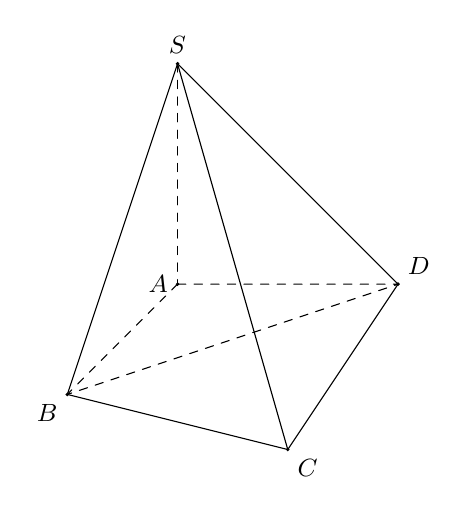
\begin{tikzpicture}[scale=0.7,every node/.style={font=\small},line cap=round,line join=round,>=stealth]
			\coordinate (A)  at (0,0);
			 \coordinate (B) at (-2,-2);
			\coordinate (C)  at (2,-3);
			 \coordinate (D) at (4,0);
			\coordinate (S) at (0,4); 
			\draw (S)--(D)  -- (C) -- (B);
			\draw (S) --  (C);
			\draw  (S) -- (B);
			 \draw[dashed] (S) -- (A);
			\draw[dashed] (A) -- (D)--(B); 
			\draw[dashed] (A)  -- (B);
			\foreach \p in  {A,B,C,D,S}{
				\fill (\p) circle (1pt); 
			} 
			 \node[left] at (A) {$A$};
			\node[below left] at  (B) {$B$};
			\node[below right] at  (C) {$C$};
			\node[above right]  at (D) {$D$};
			\node[above] at  (S) {$S$};
		\end{tikzpicture}
	} 
	 \choice
		 {\True $\dfrac{20\sqrt{273}}{819}$}
		{$\dfrac{\sqrt{91}}{9}$} 
		 {$\dfrac{3\sqrt{273}}{20}$}
		{$\dfrac{9\sqrt{91}}{9}$} 
	\loigiai{ 
	 \immini
		{ 
		Ta có $$V_{S.ABCD}=\dfrac{1}{3}SA\cdot S_{ABCD}\Leftrightarrow 66\sqrt{3}=\dfrac{1}{3}\cdot 9\cdot S_{ABCD}\Rightarrow S_{ABCD}=44\sqrt{3}.$$ 
		Suy ra $\dfrac{1}{2}AB\cdot AD+\dfrac{1}{2}BC\cdot  CD=44\sqrt{3}\Leftrightarrow 5AD+3CD=44$. (1)\\
		Áp dụng định lí  Pitago trong $2$ tam giác vuông $ABD$; $BCD$ ta có
		$$AB^2+AD^2=BD^2=BC^2+CD^2\Leftrightarrow  CD^2-AD^2=48.\quad (2)$$
		 }
		{ 
		\begin{tikzpicture}[scale=0.5,every node/.style={font=\small},line cap=round,line join=round,>=stealth]
				\coordinate (A)  at (0,0);
				 \coordinate (B) at (-2,-2);
				\coordinate  (C) at (2,-3);
				\coordinate (D) at (4,0); 
				\coordinate (S) at (0,4); 
				\coordinate  (H) at ($(B)!.5!(D)$);
				\draw  (S)--(D) -- (C) -- (B);
				 \draw (S) -- (C);
				\draw (S)  -- (B);
				\draw[dashed] (S)  -- (A)--(H);
				\draw[dashed] (A) -- (D)--(B); 
				\draw[dashed] (A)  -- (B);
				\foreach \p  in {A,B,C,D,S,H}{
					\fill (\p) circle  (1pt);
				 }
				\node[left] at (A)  {$A$};
				\node[below left] at (B)  {$B$};
				\node[below right] at (C)  {$C$};
				 \node[above right] at (D) {$D$};
				 \node[above] at (S) {$S$};
				 \node[below] at (H) {$H$};
			\end{tikzpicture}
		 }
		\noindent 
		Từ $(1)$ và $(2)$ suy ra $\hoac{& 
		 AD=4\\&
		AD=\dfrac{47}{2}.}$\\ 
		Ta có $AD=\dfrac{47}{2}$ không thỏa mãn do từ $(1)$ ta có $AD  <\dfrac{44}{5}\Rightarrow AD=4$.\\
		Trong tam giác $ABD$, dựng $AH\perp BD$ lại có $SA\perp BD\Rightarrow  BD\perp SH$.\\
		Vậy góc giữa $(SBD)$ và  đáy là góc $\widehat{SHA}$.\\
		Dễ tính $BD=\sqrt{91}$, $AH=\dfrac{AB\cdot AD}{BD}=\dfrac{20\sqrt{273}}{91}$.\\ Vậy  $\cot\widehat{SHA}=\dfrac{AH}{SA}=\dfrac{20\sqrt{273}}{819}$.
	} 
\end{ex}

% nguồn: Ok_Toan11_TracNghiem_Lan2
\begin{ex}%[1H8V7-3]%[ma:ea3e84b1]
	Cho hình chóp tứ giác $ S.ABCD $ có đáy $ ABCD $ là hình vuông cạnh bằng $ \sqrt{2}a $. Tam giác $ SAD $ cân tại $S$ và mặt bên $  (SAD) $ vuông góc với mặt phẳng đáy. Biết thể tích khối chóp $ S.ABCD $ bằng $ \dfrac{4}{3}a^3 $. Tính khoảng cách $ h $ từ $ B $ đến mặt phẳng $ (SCD) $.
	\choice 
		{$ h = \dfrac{4}{3}a $} 
		{$ h =  \dfrac{3}{2}a $}
		{$ h = \dfrac{2\sqrt{5}}{5}a $} 
		{$  h = \dfrac{\sqrt{6}}{3}a $}
	\loigiai{ 
	\immini{Gọi $ H $ là trung điểm của $ AD $,  suy ra $ SH \perp AD $.\\
		Ta có $\heva{&(SAD) \perp (ABCD) \\& 
		(SAD) \cap (ABCD) =  AD \\&
		SH \perp AD}$. Suy ra $ SH \perp (ABCD)$.\\ 
		Ta có $ S_{ABCD} =  (\sqrt{2}a)^2 = 2a^2 $.\\
		Suy ra $ 
		SH = \dfrac{3V}{S_{ABCD}} = \dfrac{3 \cdot \dfrac{4}{3}a^3}{2a^2}  = 2a$.\\
		Gọi $I$ là hình chiếu của $H$ lên $SD$.  Ta có
		\[ 
		\mathrm d(B, (SCD)) = \mathrm  d(A, (SCD)) = 2\mathrm d(H, (SCD)) = 2IH.
		\] 
		Mà 
		\[ 
		 IH = \dfrac{SH \cdot HD}{SD} = \dfrac{SH \cdot HD}{\sqrt{SH^2 + HD^2}} = \dfrac{2a \cdot \dfrac{a\sqrt{2}}{2}}{\sqrt{(2a)^2 + \left(\dfrac{a\sqrt{2}}{2}\right)^2}} = \dfrac{a^2\sqrt{2}}{\sqrt{4a^2 + \dfrac{a^2}{2}}} = \dfrac{a^2\sqrt{2}}{\sqrt{\dfrac{9a^2}{2}}} = \dfrac{a^2\sqrt{2}}{\dfrac{3a}{\sqrt{2}}} = \dfrac{2a}{3}.
		\] 
		Vậy $ \mathrm d(B, (SCD)) = 2 \cdot \dfrac{2a}{3} = \dfrac{4a}{3}  $.}{
		\begin{tikzpicture}
				 \def\a{4}
				 \def\h{4.5}
				 \path (0:0) coordinate (A)
					++(0:\a)  coordinate (B)
					++(-130:\a/2) coordinate (C) 
					($(A)+(C)-(B)$) coordinate  (D)
					($(A)!0.5!(D)$) coordinate (H) 
					($(H)+(90:\h)$) coordinate (S) 
					(intersection of  A--C and B--D) coordinate (O);
				\draw[dashed] (B)--(A)--(D) 
					(A)--(S) 
					(S)--(H)--(C); 
				 \draw (B)--(C)--(D)
					(B)--(S) 
					(C)--(S) 
					(D)--(S); 
				\foreach \x/\g  in {A/135,D/-135,C/-45,B/45,S/90,H/135}
				\fill (\x) circle  (1pt)
					($(\g:4mm)+(\x)$) node {$\x$}; 
			\end{tikzpicture}
		} 
	 }
\end{ex}

% nguồn: Ok_Toan11_TracNghiem_Lan2
\begin{ex}%[1H8V7-3]%[ma:cc9d685b]
	Cho  hình chóp $S.ABCD$ có đáy là hình vuông cạnh $a$, mặt bên $SAB$ nằm trong mặt phẳng vuông góc với $(ABCD)$, $\widehat{SAB}=30^\circ$, $SA=2a$.
	Tính thể tích $V$ của khối chóp  $S.ABCD$.
	\choice 
		 {$V=\dfrac{\sqrt{3}a^3}{6}$}
		{$V=a^3$} 
		 {$V=\dfrac{a^3}{9}$}
		{\True $V=\dfrac{a^3}{3}$} 
	 \loigiai{
		\begin{center}
			\begin{tikzpicture}[scale=1,font=\footnotesize,line join=round,line cap=round,>=stealth]
					\coordinate[label=below:$B$]  (B) at (0,0);
					 \coordinate[label=left:$A$] (A) at (-140:3);
					\coordinate[label=right:$C$] (C)  at (4,0);
					 \coordinate[label=below:$D$] (D) at ($(C)-(B)+(A)$);
					\coordinate[label=above left:$H$] (H) at  ($(B)!1/2!(A)$);
					 \coordinate[label=above:$S$] (S) at ($(H)+(90:4)$);
					\draw  (A)--(D)--(C)--(S)--cycle (S)--(D);
					\draw[dashed]  (B)--(C)
						 (H)--(S)--(B)--(A);
					\foreach \diem in {B,A,D,C,S,H} \fill (\diem) circle  (1pt);
					\draw pic["$30^\circ$",draw,angle eccentricity=1.7,angle radius=0.5cm]{angle=H--A--S}; 
					\draw pic[draw,angle radius=0.3cm]{right  angle=B--H--S};
				\end{tikzpicture}
		\end{center}
		Gọi $H$ là hình  chiếu vuông góc của $S$ lên cạnh $AB$.\\
		Do $(SAB)\perp (ABCD)$ và $(SAB)\cap (ABCD)=AB$ nên $SH \perp (ABCD)$.\\ 
		Xét tam giác $SAH$ vuông tại $H$ ta  có
		 $$
		\sin \widehat{SAB}=\dfrac{SH}{SA}\Rightarrow SH=\sin 30^\circ \cdot SA  = a.
		$$ 
		Mặt khác, ta có $S_{ABCD}=AD^2=a^2$.\\ 
		Suy ra thể tích khối chóp là 
		 $$
		V_{S.ABCD}=\dfrac{1}{3}\cdot  S_{ABCD}\cdot SH
		= \dfrac{1}{3}\cdot a^2 \cdot  a
		=  \dfrac{a^3}{3}.
		 $$
	 }
\end{ex}

% nguồn: Ok_Toan11_TracNghiem_Lan2
\begin{ex}%[1H8V7-3]%[ma:cc40dae8]
	Cho hình chóp $S.ABCD$ có đáy $ABCD$ là hình chữ nhật có $AB=a$, $AD=2a$; $SA$ vuông góc với đáy, khoảng cách từ $A$ đến ($SCD$) bằng $\dfrac{a}{2}$. Tính thể tích  của khối chóp theo $a$.
	\choice 
		{\True  $\dfrac{4 \sqrt{15}}{45}a^3$}
		 {$\dfrac{4 \sqrt{15}}{15}a^3$}
		{$\dfrac{2  \sqrt{5}}{15}a^3$}
		 {$\dfrac{2 \sqrt{5}}{45}a^3$}
	\loigiai{ 
	\immini{Gọi $H$ là hình chiếu vuông góc của điểm $A$ trên đường thẳng  $S D$.\\
		 Ta có
		$\heva{&AH\perp SD\\&AH\perp CD}$ $\Rightarrow AH\perp  (SCD)\Rightarrow AH=\mathrm{d}(A,(SCD))$.\\
		Suy  ra $AH=\dfrac{a}{2}$.\\
		Lại có $\triangle SAD$ vuông  tại $A$ có đường cao $AH$ nên
		\begin{eqnarray*}
			\dfrac{1}{AH^2}&=&\dfrac{1}{SA^2}+\dfrac{1}{AD^2}\\ 
			\Rightarrow  \dfrac{1}{SA^2}&=&\dfrac{1}{AH^2}-\dfrac{1}{AD^2}\\
			&=&\dfrac{15}{4a^2}\\ 
			\Rightarrow SA&=&\dfrac{2a \sqrt{15}}{15} 
		\end{eqnarray*}
		Vậy $V=\dfrac{1}{3}AB  \cdot AD \cdot SA=\dfrac{1}{3}a \cdot 2a \cdot \dfrac{2a \sqrt{15}}{15}=\dfrac{4 \sqrt{15}}{45}a^3$.
		}{	\begin{tikzpicture}[scale=0.7,font=\footnotesize,line join=round,line cap=round,>=stealth]
		 \path
			 (0,0) coordinate (A)
			++(-140:2)  coordinate (B)
			++(0:3.5)  coordinate (C)
			($(A)+(C)-(B)$) coordinate (D) 
			 ($(A)+(0,3)$) coordinate (S)
			($(S)!(A)!(D)$) coordinate  (H);
		\foreach \i in{B,C,D}{\draw (S)--(\i);}; 
		 \draw (B)--(C)--(D);
		\draw[dashed]  (S)--(A)--(B)
			 (A)--(D)
			(A)--(H); 
		\pic[draw,angle  eccentricity=1.8,angle radius=2mm]{right angle=S--A--D};
		 \foreach \i/\g in {A/-90,B/-90,C/-90,D/-90,S/90,H/45}
		\fill (\i) circle  (1pt)+(\g:3mm) node[scale=1]{$\i$};
		\path pic[draw,angle radius=5pt]{right angle=  A--H--D};
	\end{tikzpicture}
		} 
	} 
\end{ex}

% nguồn: Ok_Toan11_TracNghiem_Lan2
\begin{ex}%[1H8V7-3]%[ma:185c362a]
	Cho hình chóp $S.ABCD$ có đáy $ABCD$ là hình thang vuông  tại $A$ và $B$, $BC=\dfrac{1}{2}AD=a$.
	Tam giác $SAB$ đều và nằm trong mặt  phẳng vuông góc với mặt đáy; góc giữa $SC$ và mặt phẳng $(ABCD)$ bằng $\alpha$ sao cho $\tan\alpha=\dfrac{\sqrt{15}}{5}$.
	Tính thể tích khối chóp $S.ACD$ theo $a$. 
	 \choice
		{$\dfrac{a^3}{2}$} 
		 {$\dfrac{a^3}{3}$}
		 {$\dfrac{a^3\sqrt{2}}{6}$}
		{\True  $\dfrac{a^3\sqrt{3}}{6}$}
	\loigiai{ 
		\begin{center}
			\begin{tikzpicture}[scale=1,font=\footnotesize,line join=round,line cap=round,>=stealth]
					\coordinate[label=above right:$A$] (A) at (0,0); 
					 \coordinate[label=below left:$B$] (B) at (-135:2);
					\coordinate[label=below  right:$C$] (C) at (-50:2);
					\coordinate[label=right:$D$] (D) at (4,0); 
					 \coordinate[label=above:$S$] (S) at (100:3);
					\coordinate[label=left:$M$] (M) at ($(A)!0.5!(B)$); 
					\coordinate[label=above:$N$] (N) at ($(A)!0.65!(D)$); 
					 \draw (B)--(C)--(D)--(S)--cycle (B)--(S)--(C);
					\draw[dashed] (B)--(A)--(D) 
						 (M)--(S)--(A)
						 (M)--(C)--(N)
						(A)--(C); 
					\foreach  \diem in {A,B,C,D,S,M,N} \fill (\diem) circle (1pt);
					\draw pic[draw,angle radius=0.2cm]{right angle=A--M--S}; 
					\draw pic[draw,angle radius=0.2cm]{right angle=A--N--C}; 
				\end{tikzpicture}
		\end{center}
		Đặt $AB=x>0$, gọi $M$,  $N$ lần lượt là trung điểm $AB$, $AD$.\\
		Tam giác $SAB$ đều và $(SAB)\perp (ABCD)$ nên $SM$ chính là đường cao của  hình chóp $S.ABCD$.\\
		Ta có $BM=\dfrac{x}{2}$, do  đó
		$SM=\dfrac{x\sqrt{3}}{2}$.\\ 
		Suy ra  $CM=\sqrt{a^2+\dfrac{x^2}{4}}$.\\
		 Theo giả thiết, ta có $\tan\alpha=\dfrac{\sqrt{15}}{5}=\dfrac{SM}{CM}$.\\
		Khi đó, ta được 
		 \allowdisplaybreaks
		\begin{eqnarray*}
			\dfrac{SM}{CM}=\dfrac{\sqrt{15}}{5} 
			&\Rightarrow& SM^2=\dfrac{3}{5}CM^2\\ 
			&\Leftrightarrow&\dfrac{3}{4}x^2=\dfrac{3}{5}\cdot\left(a^2+\dfrac{x^2}{4}\right)\\ 
			&\Rightarrow&  x=a.
		\end{eqnarray*}
		Khi đó $ABCN$ là hình vuông nên  $CN=a$.\\
		Ta  có
		$$ 
		S_{ACD}=\dfrac{1}{2}AD\cdot CN = a^2. 
		 $$
		Do  đó thể tích cần tìm là
		 $$
		V_{S.ACD}=\dfrac{1}{3}\cdot SM\cdot S_{ACD} 
		=\dfrac{1}{3}\cdot \dfrac{a\sqrt{3}}{2}\cdot  a^2
		=\dfrac{a^3\sqrt{3}}{6}. 
		$$ 
	 }
\end{ex}

% nguồn: Ok_Toan11_TracNghiem_Lan2
\begin{ex}%[1H8V7-3]%[ma:3514273e]
	 Cho khối chóp tứ giác đều $S.ABCD$ có cạnh đáy bằng $a$, góc giữa mặt bên và mặt đáy bằng $60^\circ$.
	 Thể tích $V$ của khối chóp $S.ABCD$ bằng
	\choice 
		 {$\dfrac{a^3\sqrt{3}}{2}$}
		{$\dfrac{a^3\sqrt{2}}{2}$} 
		{\True $\dfrac{a^3\sqrt{3}}{6}$} 
		{$\dfrac{a^3\sqrt{2}}{6}$} 
	 \loigiai{
		\begin{center}
			\begin{tikzpicture}[scale=1,font=\footnotesize,line join=round,line cap=round,>=stealth]
					\coordinate[label=below left:$A$]  (A) at (0,0);
					\coordinate[label=below:$B$] (B) at  (-40:3);
					 \coordinate[label=above right:$D$] (D) at (4,0);
					 \coordinate[label=right:$C$] (C) at ($(D)-(A)+(B)$);
					\coordinate[label=below:$O$] (O) at ($(A)!.5!(C)$); 
					 \coordinate[label=above:$S$] (S) at ($(O)+(90:4)$);
					\coordinate[label=below left:$M$] (M) at  ($(A)!.5!(B)$);
					 \draw (A)--(B)--(C)--(S)--cycle (M)--(S)--(B);
					\draw[dashed] (B)--(D)--(A)--(O)--(M) 
						(S)--(O)--(C)--(D)--cycle; 
					\foreach \diem in {A,B,C,D,O,S,M} \fill (\diem) circle (1pt); 
					\draw pic[draw,angle radius=0.3cm]{right angle=S--O--M}; 
				\end{tikzpicture}
		\end{center}
		Gọi $O$ là tâm của đáy, $M$ là trung điểm  của $AB$.\\
		 Ta có
		$ 
		 \heva{
		 &SO \perp AB\\
		 &OM \perp AB
		} 
		 \Rightarrow AB\perp (SOM)$.\\
		Suy  ra $\left(\widehat{(SAB),(ABCD)}\right)= \widehat{(SM,OM)} = \widehat{SMO} = 60^\circ$.\\
		Mặt khác, ta có $OM = \dfrac{1}{2}AB = \dfrac{a}{2}$.\\ 
		Khi đó, ta được 
		 $$
		SO = OM \cdot \tan 60^\circ = \dfrac{a}{2}\cdot \sqrt{3} = \dfrac{a\sqrt{3}}{2}. 
		 $$
		Diện tích đáy là $S_{ABCD} = a^2$.\\ 
		Vậy thể  tích khối chóp là
		 $$
		V_{S.ABCD} = \dfrac{1}{3}\cdot  SO \cdot S_{ABCD}
		=  \dfrac{1}{3}\cdot \dfrac{a\sqrt{3}}{2}\cdot a^2
		=  \dfrac{a^3\sqrt{3}}{6}.
		$$ 
	 }
\end{ex}

% nguồn: Ok_Toan11_TracNghiem_Lan2
\begin{ex}%[1H8V7-3]%[ma:c22d76df]
	Cho hình chóp tứ giác đều $S.ABCD$ có cạnh đáy bằng  $a\sqrt{6}$, góc giữa cạnh bên và mặt đáy bằng $60^\circ$. Tính thể tích $V$ của khối chóp $S.ABC$.
	 \choice
		{$V=9a^3$} 
		 {$V=2a^3$}
		 {$V=3a^3$}
		{\True $V=6a^3$} 
	\loigiai{ 
	\immini{ 
		Diện tích  đáy là $S_{ABCD}=AB^2=\left(a\sqrt{6}\right)^2=6a^2$.\\
		Vì  $SO\perp (ABCD)$ nên $\left(SD,(ABCD)\right)=\widehat{SDO}\Rightarrow \widehat{SDO}=60^\circ$.\\
		 Do $ABCD$ là hình vuông nên $DO=\dfrac{1}{2}BD=\dfrac{1}{2}AB\sqrt{2}=a\sqrt{3}$.\\
		Xét  tam giác vuông $SOD$, có $$SO=DO\cdot \tan \widehat{SDO}=a\sqrt{3}\cdot \tan{60^\circ}=3a.$$
		Vậy $V_{S.ABCD}=\dfrac{1}{3}  SO\cdot S_{ABCD}=\dfrac{1}{3}\cdot 3a\cdot 6a^2=6a^3$.
		}{ 
		\begin{tikzpicture}[scale=0.9,>=stealth,line join=round,line cap=round,font=\footnotesize]
				\def\a{4} 
				 \def\h{4}
				 \def\r{2}
				\def\al{-145} 
				\path 
					(0,0) coordinate (A) 
					(\al:\r) coordinate (B) 
					 (\a,0) coordinate (D)
					 ($(B)+(D)-(A)$) coordinate (C)
					($(A)!1/2!(C)$) coordinate (O) 
					($(O)+(0,\h)$)  coordinate (S);
				 \draw (S)--(B)--(C)--(S)--(D)--(C);
				\draw[dashed,thin]  (B)--(A)--(S)--(O)
					 (C)--(A)--(D)--(B);
				\foreach \p/\g in {A/160,B/-120,C/-45,D/0,S/90,O/-90}\fill (\p) circle (1pt)  node[shift={(\g:.3)}]{$\p$};
				 \foreach \a/\b/\c in {S/O/A}
					{\draw pic[draw,angle radius=2mm] {right angle =  \a--\b--\c};};
			\end{tikzpicture}
		 }
	 }
\end{ex}

% nguồn: Ok_Toan11_TracNghiem_Lan2
\begin{ex}%[1H8V7-3]%[ma:77f4c544]
	Cho khối chóp  $S.ABCD$ có đáy là hình vuông cạnh $a$, $SA$ vuông góc với đáy và khoảng cách từ $A$ đến mặt phẳng $(SBC)$ bằng $\dfrac{a\sqrt{2}}{2}$. Tính thể tích của khối chóp đã cho.
	 \choice
		 {\True $V=\dfrac{a^3}{3}$}
		{$V=a^3$} 
		 {$V=\dfrac{\sqrt{3}a^3}{9}$}
		{$V=\dfrac{a^3}{2}$} 
	\loigiai{ 
		\begin{center}
			\begin{tikzpicture}[scale=1,font=\footnotesize,line join=round,line cap=round,>=stealth]
					\coordinate[label=left:$A$] (A)  at (0,0);
					 \coordinate[label=left:$D$] (D) at (-110:3);
					\coordinate[label=right:$B$] (B)  at (4,0);
					\coordinate[label=right:$C$]  (C) at ($(B)-(A)+(D)$);
					 \coordinate[label=above left:$S$] (S) at ($(A)+(90:4)$);
					 \coordinate[label=above right:$H$] (H) at ($(S)!(A)!(B)$);
					 \draw (D)--(C)--(B)--(S)--cycle (S)--(C);
					\draw[dashed]  (A)--(B)
						(S)--(A)--(D) 
						 (A)--(H);
					\foreach \diem in {A,D,C,B,S,H} \fill (\diem)  circle (1pt);
					 \draw pic[draw,angle radius=0.3cm]{right angle=B--A--S};
					 \draw pic[draw,angle radius=0.3cm]{right angle=A--H--B};
				\end{tikzpicture}
		\end{center}
		Vì $SA \perp (ABCD)$ nên  $SA \perp BC$.\\
		Mặt khác, ta có $BC  \perp AB$ (do $ABCD$ là hình vuông).\\
		Suy  ra $BC \perp (SAB)$.\\
		Trong  mặt phẳng $(SAB)$, kẻ $AH \perp SB$ tại $H$.
		Suy ra $AH \perp (SBC)$.\\ 
		Do đó khoảng cách từ $A$ đến mặt phẳng $(SBC)$  chính là $AH$.\\
		Theo giả thiết, ta có $\mathrm{d}(A,(SBC)) = AH = \dfrac{a\sqrt{2}}{2}$.\\ 
		Xét tam  giác $SAB$ vuông tại $A$, ta có
		\allowdisplaybreaks 
		\begin{eqnarray*}
			&&\dfrac{1}{AH^2} = \dfrac{1}{SA^2} + \dfrac{1}{AB^2}\\ 
			&\Leftrightarrow&\dfrac{1}{SA^2}=\dfrac{1}{AH^2}-\dfrac{1}{AB^2}\\  &\Leftrightarrow& \dfrac{1}{SA^2} = \dfrac{2}{a^2} - \dfrac{1}{a^2}\\
			&\Rightarrow&  SA = a.
		\end{eqnarray*}
		Diện tích  đáy là $S_{ABCD} = a^2$.\\
		Thể tích  khối chóp là
		$$V_{S.ABCD} = \dfrac{1}{3}\cdot  S_{ABCD} \cdot SA = \dfrac{1}{3}\cdot a^2 \cdot a = \dfrac{a^3}{3}.$$
	 }
\end{ex}

% nguồn: Ok_Toan11_TracNghiem_Lan2
\begin{ex}%[1H8V7-3]%[ma:cbd89371]
	Cho khối chóp $S.ABCD$ có đáy là hình vuông cạnh $a\sqrt{2}$, tam giác $SAC$  vuông tại $S$ và nằm trong mặt phẳng vuông góc với đáy, cạnh bên $SA$ tạo với đáy góc $60^\circ$. Tính thể tích $V$ của khối chóp $S.ABCD$.
	\choice 
		{$V=\dfrac{a^3\sqrt{3}}{12}$} 
		 {\True $V=\dfrac{a^3\sqrt{3}}{3}$}
		 {$V=\dfrac{a^3\sqrt{6}}{12}$}
		 {$V=\dfrac{a^3\sqrt{2}}{12}$}
	 \loigiai{
		\begin{center}
			\begin{tikzpicture}[scale=1,font=\footnotesize,line join=round,line cap=round,>=stealth]
					\coordinate[label=left:$A$] (A) at  (0,0);
					\coordinate[label=left:$B$] (B)  at (-140:3);
					 \coordinate[label=below:$D$] (D) at (4,0);
					\coordinate[label=right:$C$] (C) at ($(D)-(A)+(B)$); 
					 \coordinate[label=left:$H$] (H) at ($(A)!1/2!(C)$);
					\coordinate[label=above  left:$S$] (S) at ($(H)+(90:4)$);
					\draw (B)--(C)--(D)--(S)--cycle  (S)--(C);
					\draw[dashed]  (C)--(A)--(D)
						(H)--(S)--(A)--(B); 
					\foreach \diem in {A,B,C,D,S,H} \fill  (\diem) circle (1pt);
					 \draw pic[draw,angle radius=0.3cm]{right angle=S--H--C};
				\end{tikzpicture}
		\end{center}
		Diện tích đáy hình vuông là $S_{ABCD} = (a\sqrt{2})^2  = 2a^2$.\\
		Đường chéo của  đáy là $AC = 2a$.\\
		Trong mặt phẳng $(SAC)$, kẻ $SH  \perp AC$ tại $H$.\\
		Vì $(SAC) \perp (ABCD)$ theo giao tuyến $AC$, nên $SH \perp (ABCD)$.\\ Vậy $SH$ là chiều  cao của khối chóp.\\
		Góc giữa $SA$ và mặt phẳng đáy là góc giữa $SA$ và hình chiếu $AH$ của nó, tức  là $\widehat{SAH} = 60^\circ$.\\
		Trong tam giác vuông $SAH$, ta có $AH = SA\cdot\cos60^{\circ}$  $(1)$ \\
		Trong tam giác $SAC$ vuông tại $S$, ta có $SA^2 =  AH \cdot AC$ $(2)$\\
		Từ $(1)$ và $(2)$ ta  được
		$$SA = \cos 60^\circ\cdot AC = \dfrac{1}{2} \cdot 2a  = a.$$
		Xét tam  giác vuông $SAH$, ta được
		$$SH = SA \cdot \sin60^\circ = a \cdot \dfrac{\sqrt{3}}{2} = \dfrac{a\sqrt{3}}{2}.$$ 
		 Vậy thể tích khối chóp là
		 $$V = \dfrac{1}{3}\cdot S_{ABCD} \cdot SH = \dfrac{1}{3}\cdot 2a^2\cdot\left(\dfrac{a\sqrt{3}}{2}\right) = \dfrac{a^3\sqrt{3}}{3}.$$
	} 
\end{ex}

% nguồn: Ok_Toan11_TracNghiem_Lan2
\begin{ex}%[1H8C7-3]%[ma:653a524f]
	Cho hình chóp tứ giác đều  $S.ABCD$ có cạnh đáy bằng $a$, tâm của đáy là $O$.
	Gọi $M$ và $N$ lần lượt là trung điểm của $SA$ và $BC$. 
	Biết góc giữa đường thẳng $MN$ và mặt phẳng  $(ABCD)$ bằng $60^\circ$.
	 Thể tích khối chóp $S.ABCD$ bằng
	 \choice
		 {$\dfrac{a^3\sqrt{10}}{6}$}
		 {\True $\dfrac{a^3\sqrt{30}}{2}$}
		{$\dfrac{a^3\sqrt{30}}{6}$} 
		 {$\dfrac{a^3\sqrt{10}}{3}$}
	 \loigiai{
		\begin{center}
			\begin{tikzpicture}[scale=1,font=\footnotesize,line join=round,line cap=round,>=stealth]
					\coordinate[label=below left:$A$]  (A) at (0,0);
					\coordinate[label=below:$B$] (B)  at (-50:3);
					 \coordinate[label=above right:$D$] (D) at (4,0);
					\coordinate[label=right:$C$] (C)  at ($(D)-(A)+(B)$);
					\coordinate[label=below:$O$]  (O) at ($(A)!.5!(C)$);
					\coordinate[label=above:$S$]  (S) at ($(O)+(90:4)$);
					\coordinate[label=above:$M$]  (M) at ($(S)!.5!(A)$);
					\coordinate[label=below:$N$] (N) at  ($(B)!.5!(C)$);
					\coordinate[label=below left:$H$] (H)  at ($(A)!.5!(O)$);
					\draw  (A)--(B)--(C)--(S)--cycle (S)--(B);
					\draw[dashed]  (B)--(D)--(A)--(O)
						(S)--(O)--(C)--(D)--cycle  (M)--(H)--(N)--cycle;
					\foreach \diem in {A,B,C,D,O,S,M,N,H}  \fill (\diem) circle (1pt);
					\draw  pic[draw,angle radius=0.2cm]{right angle=S--O--A};
				\end{tikzpicture}
		\end{center}
		Gọi $H$ là trung điểm của $AO$. Khi đó góc giữa $MN$ và $(ABCD)$ chính  là $\widehat{MNH}$.\\
		Ta  có
		 $$
		HN = \sqrt{CN^2 + CH^2 - 2 \cdot CN \cdot CH  \cdot \cos 45^\circ}
		=  \dfrac{a\sqrt{10}}{4}.
		$$ 
		Suy  ra
		$$ 
		MH = HN \cdot \tan  60^\circ
		= \dfrac{a\sqrt{10}}{4}  \cdot \sqrt{3}
		=  \dfrac{a\sqrt{30}}{4}.
		 $$
		 Do đó
		 $$
		 SO = 2MH = \dfrac{a\sqrt{30}}{2}.
		$$ 
		Thể tích  khối chóp là
		 $$
		 V = \dfrac{1}{3} \cdot S_{ABCD} \cdot SO
		= \dfrac{1}{3} \cdot a^2 \cdot \dfrac{a\sqrt{30}}{2} 
		=  \dfrac{a^3\sqrt{30}}{6}.
		 $$
	 }
\end{ex}

% nguồn: Ok_Toan11_TracNghiem_Lan2
\begin{ex}%[1H8C7-3]%[ma:e367a63b]
	Cho hình chóp tứ giác $S.ABCD$ có đáy là hình vuông cạnh $\sqrt{2}a$. Tam giác $SAD$ cân tại $S$ và mặt bên $(SAD)$ vuông góc với mặt phẳng đáy. Biết thể tích khối chóp $S.ABCD$ bằng $\dfrac{4}{3}a^3$. Tính khoảng cách  $h$ từ $B$ đến mặt phẳng $(SCD)$.
	\choice 
		 {$h = \dfrac{3}{4}a$}
		{$h = \dfrac{2}{3}a$} 
		{\True  $h = \dfrac{4}{3}a$}
		{$h =  \dfrac{8}{3}a$}
	 \loigiai{
		\begin{center}
			\begin{tikzpicture}[scale=1,font=\footnotesize,line join=round,line cap=round,>=stealth]
					\coordinate[label=left:$A$]  (A) at (0,0);
					\coordinate[label=below:$D$] (D) at  (-120:3);
					 \coordinate[label=right:$B$] (B) at (4,0);
					\coordinate[label=below:$C$] (C) at  ($(B)-(A)+(D)$);
					\coordinate[label=above left:$I$] (I) at ($(A)!1/2!(D)$); 
					\coordinate[label=above left:$S$] (S)  at ($(I)+(90:4)$);
					 \coordinate[label=left:$H$] (H) at ($(S)!(I)!(D)$);
					\draw  (D)--(C)--(B)--(S)--cycle (S)--(C);
					 \draw[dashed] (A)--(B)--(I)--(S)--(A)--(D)
						 (I)--(H);
					\foreach \diem in {A,D,C,B,S,I,H}  \fill (\diem) circle (1pt);
					\draw pic[draw,angle  radius=0.3cm]{right angle=A--I--S};
					\draw pic[draw,angle radius=0.2cm]{right  angle=D--H--I};
				\end{tikzpicture}
		\end{center}
		Diện  tích đáy là $S_{ABCD} = (\sqrt{2}a)^2 = 2a^2$.\\
		Gọi $I$ là trung điểm của $AD$. Vì  $\triangle SAD$ cân tại $S$ nên $SI \perp AD$.\\
		Do $(SAD) \perp (ABCD)$ và $SI \perp AD$  nên $SI \perp (ABCD)$.\\
		Vậy $SI$ là chiều cao của khối  chóp.\\
		 Khi đó, ta có
		 \allowdisplaybreaks
		\begin{eqnarray*}
			V_{S.ABCD} &=& \dfrac{1}{3}\cdot  S_{ABCD} \cdot SI\\
			&\Leftrightarrow&  SI = \dfrac{3\cdot V_{S.ABCD}}{S_{ABCD}}\\
			&\Rightarrow& SI  = \dfrac{3\cdot \dfrac{4a^3}{a}}{2a^2} = 2a.
		\end{eqnarray*}
		Vì  $AB \parallel CD$ nên
		$$h =  \mathrm{d}\left(B, (SCD)\right) = \mathrm{d}\left(A, (SCD)\right).$$
		Vì $I$ là trung điểm $AD$, ta có $\mathrm{d}\left(A,  (SCD)\right) = 2 \cdot \mathrm{d}\left(I, (SCD)\right)$.\\
		Trong  mặt phẳng $(SID)$, kẻ $IH \perp SD$ tại $H$. Ta có $CD \perp AD$ và $CD \perp SI$ nên $CD \perp (SID)$.\\
		Do đó $CD  \perp IH$.\\
		Vì $IH \perp SD$ và $IH \perp  CD$ nên $IH \perp (SCD)$.\\
		Vậy $\mathrm{d}\left(I, (SCD)\right) = IH$.\\ 
		Xét tam giác  $SID$ vuông tại $I$, có $ID = \dfrac{AD}{2} = \dfrac{\sqrt{2}a}{2}$.\\
		Áp dụng hệ thức lượng vào  tam giác $SID$ ta được
		\allowdisplaybreaks 
		\begin{eqnarray*}
			\dfrac{1}{IH^2}  &=& \dfrac{1}{SI^2} + \dfrac{1}{ID^2}\\
			&=& \dfrac{1}{(2a)^2}  + \dfrac{1}{\left(\dfrac{\sqrt{2}a}{2}\right)^2} \\
			&\Rightarrow& IH = \dfrac{2a}{3}. 
		\end{eqnarray*}
		Vậy  khoảng cách cần tìm là
		$$h = \mathrm{d}\left(B, (SCD)\right) = 2 \cdot IH = 2 \cdot \dfrac{2a}{3}  = \dfrac{4a}{3}.$$
	} 
\end{ex}

% nguồn: Ok_Toan11_TracNghiem_Lan2
\begin{ex}%[1H8C7-3]%[ma:eb1aca58]
	Cho hình chóp tứ giác đều $S.ABCD$ có  cạnh đáy bằng $a$. Biết rằng mặt phẳng $(P)$ qua $A$ và vuông góc với $SC$, cắt $SB$ tại $B'$ với $\dfrac{SB'}{SB} = \dfrac{2}{3}$.
	Tính thể tích của khối chóp  $S.ABCD$.
	 \choice
		 {\True $\dfrac{a^3\sqrt{6}}{6}$}
		{$\dfrac{a^3\sqrt{6}}{4}$} 
		{$\dfrac{a^3\sqrt{6}}{2}$} 
		{$\dfrac{a^3\sqrt{6}}{3}$} 
	 \loigiai{
		\begin{center}
			\begin{tikzpicture}[scale=1,font=\footnotesize,line join=round,line cap=round,>=stealth]
					\coordinate[label=below left:$A$] (A)  at (0,0);
					\coordinate[label=below:$B$] (B) at (-40:3); 
					\coordinate[label=above right:$D$] (D) at (4,0); 
					\coordinate[label=right:$C$] (C)  at ($(D)-(A)+(B)$);
					\coordinate[label=below:$O$] (O)  at ($(A)!.5!(C)$);
					\coordinate[label=above:$S$] (S) at  ($(O)+(90:4)$);
					\coordinate[label=left:$B'$] (B') at ($(S)!2/3!(B)$); 
					\coordinate[label=right:$C'$] (C') at ($(S)!0.5!(C)$); 
					 \coordinate[label=
						above right:$G$] (G) at (intersection of A--C'  and S--O);
					 \draw (A)--(B)--(C)--(S)--cycle (S)--(B);
					\draw[dashed] (B)--(D)--(A)--(O) 
						(S)--(O)--(C)--(D)--cycle (A)--(C') 
						(G)--(B'); 
					\foreach \diem in {A,B,C,D,O,S,B',C',G}  \fill (\diem) circle (1pt);
					\draw pic[draw,angle radius=0.3cm]{right angle=S--O--A}; 
				\end{tikzpicture}
		\end{center}
		Ta có $\heva{ 
		&BD \perp  AC\\
		&BD  \perp SO} \Rightarrow BD \perp (SAC)$.\\
		Suy ra $BD  \perp SC$.\\
		Mặt khác $(P) \perp SC$  nên $(P) \parallel BD$.\\
		Trong mặt phẳng $(SAC)$, gọi  $G = AC' \cap SO$. Suy ra $GB' \parallel BD$.\\
		Khi đó, ta được  $\dfrac{SG}{SO} = \dfrac{SB'}{SB} = \dfrac{2}{3}$.\\
		Suy  ra $G$ là trọng tâm $\triangle SAC$. Ta được $C'$ là trung điểm $SC$.\\
		Suy  ra $\triangle SAC$ đều cạnh $AC = a\sqrt{2}$
		Khi đó $SO = a\sqrt{2}\cdot \dfrac{\sqrt{3}}{2} =  \dfrac{a\sqrt{6}}{2}$.\\
		Do  đó
		$$ 
		V_{S.ABCD}  = \dfrac{1}{3} \cdot S_{ABCD} \cdot SO
		= \dfrac{1}{3} \cdot a^2  \cdot \dfrac{a\sqrt{6}}{2}
		 = \dfrac{a^3 \sqrt{6}}{6}.
		$$ 
	} 
\end{ex}


%%%%%%%%%%%%%%%% ĐÚNG/SAI %%%%%%%%%%%%%%%%

% nguồn: Ok_dungsai_lop11_Lan1
\begin{ex}%[1H8H7-3]%[ma:f91e87dd]
 Cho hình chóp tứ giác  đều $S.ABCD$ có tất cả các cạnh bằng nhau và bằng $a$. Khi đó
  \choiceTF
  {\True $(SAC)\perp  (SBD)$}
  {\True Các cạnh bên  tạo với đáy một góc $45^{\circ}$}
  {\True Côsin của góc giữa mặt  bên và mặt đáy bằng $\dfrac{\sqrt{3}}{3}$}
  {Thể  tích khối chóp $S.ABCD$ bằng $\dfrac{a^3\sqrt{2}}{2}$ }
 \loigiai{ 
  \immini{
  \begin{itemchoice}
   \itemch  Đúng\\
   Gọi $O$  là tâm của $ABCD$. Khi đó $SO\perp (ABCD)$ nên $SO\perp BD$. \\
   Lại có $BD\perp  AC$ nên $BD\perp (SAC)$. Suy ra $(SBD)\perp (SAC)$.
   \itemch Đúng\\ 
   Góc giữa cạnh bên và  đáy bằng góc $\widehat{SCO}$.\\
   Ta có $SC=a$, $OC=\dfrac{a\sqrt{2}}{2}$.  Tam giác $SOC$ vuông ở $O$ nên
   \[\cos \widehat{SCO}=\dfrac{OC}{SC}=\dfrac{\sqrt{2}}{2}\Rightarrow  \widehat{SCO}=45^{\circ}.\]
   \itemch Đúng\\ 
   Gọi $M$ là trung điểm của $CD$.  Ta có
   $$\heva{&OM\perp CD\\&SO\perp  CD}\Rightarrow CD\perp (SOM)\Rightarrow CD\perp SM.$$
   Do đó góc giữa mặt bên và mặt đáy bằng góc $\widehat{SMO}$.\\ 
   Tam giác $SCD$ đều cạnh $a$  nên $SM=\dfrac{a\sqrt{3}}{2}$. Do đó
   \[\cos \widehat{SMO}=\dfrac{OM}{SM}=\dfrac{\frac{a}{2}}{\frac{a\sqrt{3}}{2}}=\dfrac{\sqrt{3}}{3}.\] 
    \itemch Sai\\
   Ta có $SO=OC=\dfrac{a\sqrt{2}}{2}$. Thể tích khối chóp $S.ABCD$  là
   \[V=\dfrac{1}{3}\cdot  SO\cdot S_{ABCD}=\dfrac{1}{3}\cdot \dfrac{a\sqrt{2}}{2}\cdot a^2=\dfrac{a^3\sqrt{2}}{6}.\]
  \end{itemchoice}}
  {\begin{tikzpicture}[>=stealth,line join=round,line cap=round,font=\footnotesize,scale=0.4]
  \clip (-5,-5) rectangle  (11,7);
   \def\r{6.5};
   \def\g{120};
   \def\gC{30};
  \path 
    (0,0) coordinate (A)
   (-4,-4)  coordinate (B)
   (6,-4)  coordinate (C)
   (10,0) coordinate (D) 
   (3,6) coordinate  (S)
   (3,-2)  coordinate (O);
   \coordinate (M) at ($(D)!0.5!(C)$);
  \draw  (S)--(B)--(C)--(D)--(S)--(C)
   (M)--(S); 
   \draw[dashed] (B)--(A)--(S)
   (B)--(D)--(A)--(C) 
   (S)--(O) circle  (1pt) node[below]{$O$}--(M) circle (1pt) node[below]{$M$};
  \fill[black] (A) circle (1pt) node[above left]{$A$} 
   (C) circle (1pt) node[below right]{$C$} 
   (B) circle (1pt) node[below  left]{$B$}
   (S) circle (1pt) node[above  right]{$S$}
    (D) circle (1pt) node[below right]{$D$};
 \end{tikzpicture}
   }
 } 
\end{ex}


%%%%%%%%%%%%%%%% TRẢ LỜI NGẮN %%%%%%%%%%%%%%%%

% nguồn: Ok_TraLoiNgan_Lop11_Lan1
\begin{ex}%[1H8V7-3]%[ma:1c4afb9a]
	Cho khối chóp $S.ABCD$ có đáy là hình vuông. Cạnh bên $SA$ vuông góc với đáy, cạnh bên $SC$ tạo  với đáy góc $45^{\circ}$ và khoảng cách từ $A$ đến mặt phẳng $(SBC)$ bằng $\sqrt{2}$. Tính thể tích của khối chóp đã cho (kết quả làm tròn đến hàng phần trăm).
	\shortans{2,45} 
	\loigiai{ 
	\immini{Giả  sử $AB=a$.\\
		Vì $SA\perp(ABCD)$ nên hình chiếu của  $SC$ lên $(ABCD)$ là $AC$ \\
		$ \Rightarrow $ Góc giữa  $SC$ và $(ABCD)$ là góc $(SC,AC)$.\\
		Tam giác $SAC$ vuông tại $A$ nên $(SC,AC)=\widehat{SCA}=45^{\circ}$ \\ 
		$ \Rightarrow $ Tam giác $SAC$ vuông cân tại $A$  nên $SA=AC=a\sqrt{2}$.\\
		Ta có $BC\perp  AB$, $BC\perp SA\Rightarrow BC\perp(SAB)$.\\
		Kẻ  $AH\perp SB\Rightarrow AH\perp(SBC)$. \\
		Suy  ra $\mathrm{d}\left(A;(SBC)\right)=AH=\sqrt{2}$.\\
		}{	\begin{tikzpicture}[scale=0.9,font=\footnotesize,line join=round,line cap=round,>=stealth]
		\path 
			(0,0)  coordinate (A)
			 (-1.3,-1.6) coordinate (D)
			(2.5,-1.6) coordinate  (C)
			($(A)+(C)-(D)$) coordinate (B) 
			($(A)+(0,3)$) coordinate (S) 
			($(S)!0.55!(B)$)  coordinate (H);
		\draw  (S)--(B)--(C)--(D)--cycle (S)--(C);
		\draw[dashed]  (S)--(A)--(D)
			(C)--(A)--(B) 
			(A)--(H); 
		 \foreach \p/\q in {S/90,A/-90,D/-90,C/-90,B/0,H/50}
		\fill[black] (\p) circle (1.0pt)  node[shift={(\q:2.5mm)}]{$\p$};
	\end{tikzpicture}
		 }
		\noindent 
		Tam giác $SAB$  vuông tại $A$ có $$\dfrac{1}{AH^2}=\dfrac{1}{SA^2}+\dfrac{1}{AB^2}\Leftrightarrow\dfrac{1}{2}=\dfrac{1}{2a^2}+\dfrac{1}{a^2}\Leftrightarrow a=\sqrt{3}.$$
		Vậy $$V_{SABCD}=\dfrac{1}{3}SA\cdot  S_{ABCD}=\dfrac{1}{3}(a\sqrt{2})\cdot a^2=\dfrac{1}{3}\cdot\left(\sqrt{3}\cdot\sqrt{2}\right)\cdot (\sqrt{3})^2=\sqrt{6}\approx 2{,}45.$$
	 }
\end{ex}

% nguồn: Ok_TraLoiNgan_Lop11_Lan1
\begin{ex}%[1H8V7-3]%[ma:4aa772d6]
	Cho khối chóp đều $S.ABCD$ có đáy $ABCD$ là hình vuông cạnh bằng $\sqrt{6}$, góc giữa đường thẳng $SA$ và mặt phẳng $(ABCD)$ bằng $60^{\circ}$. Tính thể tích khối  chóp $S.ABCD$.
	\shortans{6} 
	 \loigiai{
	 \immini{
		Gọi  $O$ là giao điểm của $AC$ và $BD$ thì $SO \perp(ABCD)$ và góc giữa $SA$ và $(ABCD)$ bằng góc $SAO$ bằng $60^{\circ}$.\\
		Xét tam giác $SAO$ vuông tại $O$, có  $AO=\dfrac{\sqrt{6}\cdot \sqrt{2}}{2}=\sqrt{3}$ và $\widehat{SAO}=60^{\circ}$.\\
		Khi đó $SO=AO \cdot \tan \widehat{SAO}=\sqrt{3} \cdot \tan  60^{\circ}=3$.\\
		Do đó, $V_{S.ABCD}=\dfrac{1}{3} \cdot S_{ABCD} \cdot SO=\dfrac{1}{3} \cdot 6 \cdot 3=6$. 
		}{ 
		\begin{tikzpicture}[scale=1,font=\footnotesize,line join=round,line cap=round,>=stealth]
				 \path
					 (0,0) coordinate (A)
					(-1.9,-1.6)  coordinate (B)
					(1.6,-1.6) coordinate  (C)
					($(A)+(C)-(B)$) coordinate  (D)
					($(A)!0.5!(C)$)  coordinate (O)
					 ($(O)+(0,3.5)$) coordinate (S);
				 \draw (S)--(B)--(C)--(D)--cycle (S)--(C);
				\draw[dashed] (O)--(S)--(A)--(D) 
					(C)--(A)--(B)--(D); 
				\foreach  \p/\q in {S/90,A/-100,B/-90,C/-90,D/0,O/-90}
				\fill[black]  (\p) circle (1.0pt) node[shift={(\q:3mm)}]{$\p$};
				\draw pic[draw=black,angle  radius=0.2cm] {right angle = S--O--A};
				\draw pic[draw=black,angle  radius=0.2cm] {right angle = S--O--D};
			\end{tikzpicture}
		 }
	 }
\end{ex}


%%%%%%%%%%%%%%%% TỰ LUẬN %%%%%%%%%%%%%%%%

% nguồn: Ok_TuanLuan_Toan11_Lan2
\begin{ex}%[1H8N7-3]%[ma:717e9583]
	Hình chóp $S.ABCD$ có đáy hình  vuông, $SA$ vuông góc với đáy và $SA=a\sqrt{3}$, $AC=a\sqrt{2}$. Khi đó thể tích khối chóp $S.ABCD$ là
	 \loigiai{
		\begin{center}
			\begin{tikzpicture}[scale=1,font=\footnotesize,line join=round,
						 line cap=round,>=stealth]
					 \path
						(0:0) coordinate (A) 
						++(0:4)  coordinate (B)
						++(-140:2) coordinate (C) 
						($(C)-(B)+(A)$) coordinate  (D)
						($(A)+(90:3)$) coordinate (S); 
					\draw[]  (B)--(C)--(D)
						 (B)--(S)
						(C)--(S) 
						(D)--(S); 
					 \draw[dashed] (A)--(S)
						 (D)--(A)--(B)
						(A)--(C); 
					\foreach \x  /\goc in {A/180,B/0,C/-90,D/-90,S/90}
					 \fill (\x) circle (1pt)
						 ($(\x)+(\goc:3mm)$) node {$\x$};
					\foreach \x/\y/\z in {S/A/B}{\draw pic[draw,angle radius=2mm]{right  angle=\x--\y--\z};}
				\end{tikzpicture}
		\end{center}
		Vì $ABCD$ là hình vuông  có $AC=a\sqrt{2}$ nên $AB=a$.\\
		Vậy 
		$$V_{S.ABCD}=\dfrac{1}{3}SA\cdot  S_{ABCD}=\dfrac{1}{3}a\sqrt{3}\cdot a^2=\dfrac{a^3\sqrt{3}}{3}.$$
	 }
\end{ex}

% nguồn: Ok_TuanLuan_Toan11_Lan2
\begin{ex}%[1H8H7-3]%[ma:c628b47b]
	Cho khối chóp $S.ABCD$ có đáy $ABCD$ là hình vuông cạnh $a$, $SA \perp (ABCD)$. Biết  góc giữa hai mặt phẳng $(SBD)$ và $(ABCD)$ là $30^\circ$. Tính thể tích khối chóp $S.ABCD$.
	\loigiai{ 
		\begin{center}
			\begin{tikzpicture}[scale=1,font=\footnotesize,line join=round,
						line  cap=round,>=stealth]
					 \path
						(0:0)  coordinate (A)
						++(0:4) coordinate  (B)
						++(-140:2)  coordinate (C)
						($(C)-(B)+(A)$)  coordinate (D)
						(intersection of A--C and B--D)  coordinate (O)
						($(A)+(90:3)$) coordinate  (S);
					\draw[] (B)--(C)--(D) 
						 (B)--(S)
						(C)--(S) 
						 (D)--(S);
					 \draw[dashed] (A)--(S)
						(D)--(A)--(B) 
						 (A)--(C)
						(B)--(D) 
						(S)--(O); 
					\foreach \x /\goc in  {A/180,B/0,C/-90,D/-90,S/90,O/-90}
					\fill (\x) circle (1pt) 
						($(\x)+(\goc:3mm)$)  node {$\x$};
					\foreach \x/\y/\z  in {S/A/B}{\draw pic[draw,angle radius=2mm]{right angle=\x--\y--\z};}
				\end{tikzpicture}
		\end{center}
		Gọi $O$ là tâm hình  vuông $ABCD$. Khi đó $BD\perp SA$ và $BD \perp AO$.\\
		$\Rightarrow BD \perp  (SAO)$.\\
		 $\Rightarrow BD \perp AO$ và $BD \perp SO$.\\
		Do đó góc giữa hai mặt phẳng $(SBD)$ và  $(ABCD)$ là góc $\widehat{SOA}$ hay $\widehat{SOA}=30^\circ$.\\
		 Xét tam giác vuông $SAO$
		$$SA=AO \cdot  \tan \widehat{SOA}=\dfrac{1}{2}AC \cdot \tan 30^\circ=\dfrac{a\sqrt{6}}{6}.$$
		Suy ra 
		$$V_{S.ABCD}=\dfrac{1}{3}SA \cdot  S_{ABCD}
		=\dfrac{1}{3}\cdot \dfrac{a\sqrt{6}}{6}\cdot  a^2
		 =\dfrac{a^3\sqrt{6}}{18}.$$
	} 
\end{ex}

% nguồn: Ok_TuanLuan_Toan11_Lan2
\begin{ex}%[1H8H7-3]%[ma:d1d38f8a]
	Cho hình chóp $S.ABCD$, $ABCD$ là hình vuông cạnh $2a$, $SA \perp (ABCD)$. Góc giữa $SC$ và $(ABCD)$ là $60^\circ$. Tính thể  tích khối chóp $S.ABCD$.
	 \loigiai{
		\begin{center}
			\begin{tikzpicture}[scale=1,font=\footnotesize,line join=round,
						line  cap=round,>=stealth]
					 \path
						(0:0) coordinate  (A)
						++(0:4)  coordinate (B)
						 ++(-140:2) coordinate (C)
						 ($(C)-(B)+(A)$) coordinate (D)
						($(A)+(90:3)$) coordinate (S); 
					\draw[] (B)--(C)--(D) 
						 (B)--(S)
						(C)--(S) 
						(D)--(S); 
					\draw[dashed] (A)--(S) 
						 (D)--(A)--(B)
						(A)--(C); 
					\foreach \x /\goc in {A/180,B/0,C/-90,D/-90,S/90} 
					\fill (\x) circle  (1pt)
						 ($(\x)+(\goc:3mm)$) node {$\x$};
					\foreach \x/\y/\z in {S/A/B}{\draw  pic[draw,angle radius=2mm]{right angle=\x--\y--\z};}
					\draw pic[draw,angle radius=0.5cm,"$\tiny  60^\circ$",angle eccentricity=1.5]{angle=S--C--A};
				\end{tikzpicture}
		\end{center}
		Vì $SA \perp (ABCD)$  nên $AC$ là hình chiếu của $SC$ trên $(ABCD)$.
		 $\Rightarrow \widehat{SCA}=60^\circ$.\\
		$ABCD$ là  hình vuông nên $AC=\sqrt{AB^2+BC^2}=\sqrt{(2a)^2+(2a)^2}=2a\sqrt{2}$.\\
		Khi  đó $SA=AC \cdot \tan 60^\circ=2a\sqrt{2}\cdot \sqrt{3}=2a\sqrt{6}$.\\
		Thể  tích khối chóp
		$$V=\dfrac{1}{3}S_{ABCD}\cdot SA=\dfrac{1}{3}(2a)^2 \cdot  2a\sqrt{6}
		 =\dfrac{8}{3}a^3\sqrt{6}.$$
	} 
\end{ex}

% nguồn: Ok_TuanLuan_Toan11_Lan2
\begin{ex}%[1H8H7-3]%[ma:50d74616]
	Cho hình chóp tứ giác đều $S.ABCD$ có cạnh đáy bằng $20$, cạnh bên bằng $30$. Tính thể tích  $V$ của khối chóp đã cho.
	\loigiai{ 
	 \immini
		 {
		Trong mặt phẳng $ABCD$,  gọi $O=AC\cap BD$, do hình chóp $S.ABCD$ là hình chóp tứ giác đều nên $SO\perp(ABCD)$.\\
		Đáy là hình vuông cạnh $20 \Rightarrow AO=\dfrac{AC}{2}=10\sqrt{2}$.\\ 
		 Trong tam giác vuông $SAO$ có $SO=\sqrt{SA^2-AO^2}=10\sqrt{7}$.\\
		Thể tích $V$ của khối chóp trên  là $$V=\dfrac{1}{3}SO\cdot S_{ABCD}=\dfrac{1}{3}\cdot 10\sqrt{7}\cdot 400=\dfrac{4\,000 \sqrt{7}}{3}.$$
		} 
		 {
		\begin{tikzpicture}[>=stealth,line join=round,line cap=round,font=\footnotesize,scale=1]
				 \path
					(0,0) coordinate (A) 
					 (30:1.5) coordinate (B)
					(2.5,0) coordinate (D) 
					($(B)+(D)-(A)$) coordinate (C) 
					($(A)!0.5!(C)$) coordinate (O) 
					($(O)+(0,2.5)$)  coordinate (S);
				\draw  (S)--(A)--(D)--(C)--cycle
					(S)--(D); 
				\draw[dashed](S)--(B)--(C) 
					 (D)--(B)--(A)--(C)
					(O)--(S); 
				\foreach \x/\g in  {A/-90,C/0,D/-90,B/180,S/90,O/-90}\fill(\x) circle (1pt)+(\g:.2) node[scale=0.8]{$\x$};
			\end{tikzpicture}
		} 
	} 
\end{ex}

% nguồn: Ok_TuanLuan_Toan11_Lan2
\begin{ex}%[1H8H7-3]%[ma:19f69755]
	Cho hình  chóp đều $S.ABCD$ có cạnh đáy bằng $a$, cạnh bên hợp với mặt đáy một góc $60^{\circ}$. Tính thể tích $V$ của khối chóp $S.ABCD$.
	\loigiai{ 
	\immini{Gọi $O$ là giao điểm của $AC$  và $BD$.\\
		 Do $S.ABCD$ là hình chóp đều nên $SO\perp(ABCD)$.\\
		Suy ra $OB$ là hình chiếu của  $SB$ trên $(ABCD)$.\\
		Khi  đó $60^{\circ}=\left(SB,(ABCD)\right)=\left(SB,OB\right)=\widehat{SBO}$.\\
		Tam giác  vuông $SOB$, có $SO=OB\cdot\tan \widehat{SBO}=\dfrac{a\sqrt{6}}{2}$.\\
		Diện tích hình vuông $ABC$ là $S_{ABCD}=AB^2=a^2$. 
		}{ 
		\begin{tikzpicture}[scale=1,font=\footnotesize,line join=round,line cap=round,>=stealth]
				\def  \r{2.5}
				\path 
					(0,0) coordinate (A) 
					(0:\r) coordinate (B) 
					(220:0.55*\r) coordinate  (D)
					($(B)+(D)$) coordinate  (C)
					($(B)!0.5!(D)$) coordinate (O) 
					($(A)!(O)!(B)$) coordinate (M) 
					 ($(M)!1.1!90:(B)$) coordinate (S);
				 \draw (S)--(B)--(C)--(D)--(S)--(C);
				 \draw[dashed] (B)--(A)--(D)
					(S)--(A)--(C) 
					 (B)--(D)
					(S)--(O); 
				\foreach \x/\g  in {S/160,A/180,B/0,C/-60,D/180,O/-90}\fill (\x) circle (1pt)+(\g:.3) node{$\x$};
			\end{tikzpicture}
		 }
		\noindent Vậy $V_{S.ABCD}=\dfrac{1}{3}S_{ABCD}\cdot  SO=\dfrac{a^3\sqrt{6}}{6}$.
	 }
\end{ex}

% nguồn: Ok_TuanLuan_Toan11_Lan2
\begin{ex}%[1H8H7-3]%[ma:b7b040a3]
	Cho hình chóp $S.ABCD$ có đáy $ABCD$ là hình vuông, cạnh bên $SA=a\sqrt{2}$ và $SA$ vuông góc với mặt phẳng đáy, tam giác $SBD$ là tam giác đều. Tính thể tích  của khối chóp $S.ABCD$.
	\loigiai{ 
		\begin{center}
			\begin{tikzpicture}[scale=1,font=\footnotesize,line join=round,
						line  cap=round,>=stealth]
					\path 
						 (0:0) coordinate (A)
						 ++(0:4) coordinate (B)
						 ++(-140:2) coordinate (C)
						($(C)-(B)+(A)$)  coordinate (D)
						 ($(A)+(90:3)$) coordinate (S);
					\draw[] (B)--(C)--(D) 
						 (B)--(S)
						(C)--(S) 
						(D)--(S); 
					\draw[dashed]  (A)--(S)
						 (D)--(A)--(B)
						(B)--(D); 
					\foreach \x /\goc in {A/180,B/0,C/-90,D/-90,S/90} 
					 \fill (\x) circle (1pt)
						 ($(\x)+(\goc:3mm)$) node {$\x$};
					\foreach \x/\y/\z in {S/A/B}{\draw pic[draw,angle radius=2mm]{right  angle=\x--\y--\z};}
				\end{tikzpicture}
		\end{center}
		 Đặt $AB=x$. Tam giác $ABD$ vuông cân tại $A$ nên $BD=x\sqrt{2}$.\\
		 Vì $\triangle SBD$ đều nên $SB=SD=BD=x\sqrt{2}$.\\
		Lại có $\triangle SAB$ vuông tại  $A$ nên
		\begin{eqnarray*}
			 &&SA^2+AB^2=SB^2\\
			 &&\left(a\sqrt{2}\right)^2+x^2=\left(x\sqrt{2}\right)^2\\
			 &&x^2=2a^2\\
			&&\Rightarrow  x=a\sqrt{2}.
		\end{eqnarray*}
		Diện  tích đáy
		$$S_{ABCD}=AB^2=(a\sqrt{2})^2=2a^2.$$ 
		Thể  tích khối chóp
		 $$V_{S.ABCD}=\dfrac{1}{3}SA \cdot S_{ABCD}=\dfrac{1}{3}a\sqrt{2}\cdot 2a^2=\dfrac{2a^3\sqrt{2}}{3}.$$
	 }
\end{ex}

% nguồn: Ok_TuanLuan_Toan11_Lan2
\begin{ex}%[1H8H7-3]%[ma:ff017dcc]
	Cho hình chóp $S.ABCD$ có đáy $ABCD$ là hình thoi cạnh $a$ và  góc $\widehat{BAD}=60^{\circ}$,\\ $SA \perp (ABCD)$, $SA=\dfrac{a\sqrt{6}}{2}$. Thể tích khối chóp $S.ABCD$ là
	\loigiai{ 
		\begin{center}
			\begin{tikzpicture}[scale=1,font=\footnotesize,line join=round,
						 line cap=round,>=stealth]
					 \path
						(0:0) coordinate (A) 
						++(0:4) coordinate  (B)
						 ++(-140:2) coordinate (C)
						($(C)-(B)+(A)$)  coordinate (D)
						(intersection of A--C and B--D)  coordinate (O)
						($(A)+(90:3)$) coordinate (S); 
					 \draw[] (B)--(C)--(D)
						(B)--(S) 
						(C)--(S) 
						(D)--(S); 
					\draw[dashed] (A)--(S) 
						 (D)--(A)--(B)
						 (A)--(C)
						 (B)--(D);
					\foreach \x /\goc  in {A/180,B/0,C/-90,D/-90,S/90,O/-90}
					\fill  (\x) circle (1pt)
						 ($(\x)+(\goc:3mm)$) node {$\x$};
					\foreach \x/\y/\z in  {S/A/B}{\draw pic[draw,angle radius=2mm]{right angle=\x--\y--\z};}
				\end{tikzpicture}
		\end{center}
		Vì hình thoi có  $\widehat{BAD}=60^{\circ}$ nên tam giác $ABD$ đều, cạnh bằng $a$.
		 $$S_{ABCD}=2S_{ABD}=2\cdot \dfrac{a^2\sqrt{3}}{4}=\dfrac{a^2\sqrt{3}}{2}.$$
		Thể tích khối  chóp
		$$V_{S.ABCD}=\dfrac{1}{3}\,S_{ABCD}\cdot SA 
		=\dfrac{1}{3}\cdot \dfrac{a^2\sqrt{3}}{2}\cdot \dfrac{a\sqrt{6}}{2} 
		 =\dfrac{a^3\sqrt{2}}{4}.$$
	 }
\end{ex}

% nguồn: Ok_TuanLuan_Toan11_Lan2
\begin{ex}%[1H8H7-3]%[ma:9f5df00b]
	Tính thể tích khối chóp tứ giác đều  $S.ABCD$ có cạnh đáy bằng $a$ và góc giữa mặt bên và mặt phẳng chứa đa giác đáy bằng $60^\circ$.
	\loigiai{ 
	\immini{ 
		Gọi $O$ là tâm  của đáy, gọi $I$ là trung điểm của $BC$.\\
		Ta  có $\heva{&SO\perp BC\\&OI\perp BC\\&SO\cap OI=I}$
		nên  $(SOI) \perp BC$.\\
		Suy ra  \[\left[(SBC),(ABCD)\right]=(SI, OI)=\widehat{SIO}=60^{\circ}.\]
		}{ 
		\begin{tikzpicture}[declare function={goc=-150; a=5; b=a/2; h=4;},scale=0.7,font=\footnotesize,line cap=round,line join=round]
				\path (0,0) coordinate  (A)
					(a,0) coordinate  (B)
					(goc:b)  coordinate (D)
					 +(a,0) coordinate (C)
					($(A)!.5!(C)$)  coordinate (O)
					+(0,h) coordinate (S) 
					 ($(B)!.5!(C)$) coordinate (I);
				\draw pic[angle  radius=3mm,draw] {right angle = S--O--D};
				\draw[dashed]  (S)--(A)
					 (D)--(A)--(B)
					 (S)--(O)
					(A)--(C) 
					(D)--(B) 
					 (O)--(I);
				\draw (S)--(D)--(C)--(S)--(B)--(C)--cycle  (S)--(I);
				\foreach  \x/\goc in {S/90,A/150,B/0,C/-60,D/-180,O/-90,I/0}
				\draw[fill] (\x) node[shift={(\goc:7pt)},font=\scriptsize]{$\x$} circle (1pt); 
			\end{tikzpicture}
		 }
		\noindent 
		 Ta có $OI=\dfrac{1}{2} BC=\dfrac{a}{2}$, $SO=OI\cdot \tan 60^{\circ}=\dfrac{a \sqrt{3}}{2}$.\\
		Thể tích  khối chóp $S.ABCD$ là
		 $V_{S. ABCD}=\dfrac{1}{3} SO\cdot S_{ABCD}=\dfrac{1}{3} \cdot \dfrac{a \sqrt{3}}{2} \cdot a^2=\dfrac{a^3\sqrt{3}}{6}$.
	 }
\end{ex}

% nguồn: Ok_TuanLuan_Toan11_Lan2
\begin{ex}%[1H8H7-3]%[ma:82841306]
	Cho hình chóp $S.ABCD$ có đáy $ABCD$ là hình vuông có cạnh $\sqrt{3}  a$ tâm $O$, $SO$ vuông góc với $(ABCD)$, $SO=a$. Tính thể tích của khối chóp $S.ABCD$.
	 \loigiai{
	\immini 
		{ 
		Diện tích mặt đáy  $ABCD$ là $S_{ABCD}=3a^2$.\\
		Thể tích khối chóp $S.ABCD$ là $V=\dfrac{1}{3}\cdot SO\cdot S_{ABCD}=\dfrac{1}{3}\cdot a\cdot 3a^2=a^3$. 
		} 
		{ 
		\begin{tikzpicture}[scale=0.7,font=\footnotesize,line join=round,line cap=round,>=stealth]
				 \def\bc{4}
				 \def\ba{2}
				 \def\h{4}
				\def\gocB{30} 
				\coordinate[label=below left:$B$]  (B) at (0,0);
				\coordinate[label=above right:$A$] (A) at  (\gocB:\ba);
				 \coordinate[label=below:$C$] (C) at (\bc,0);
				 \coordinate[label=right:$D$] (D) at ($(C)-(B)+(A)$);
				\coordinate[label=below:$O$] (O) at ($(A)!.5!(C)$); 
				 \coordinate[label=above:$S$] (S) at ($(O)+(90:\h)$);
				\draw (B)--(C)--(D)--(S)--cycle (S)--(C); 
				\draw[dashed] (C)--(A)--(D)--(B) 
					(O)--(S)--(A)--(B); 
				\foreach \diem in {A,B,C,D,S,O}  \fill (\diem) circle (1pt);
			\end{tikzpicture}
		} 
	 }
\end{ex}

% nguồn: Ok_TuanLuan_Toan11_Lan2
\begin{ex}%[1H8H7-3]%[ma:21f06c84]
	Cho khối chóp $S.ABCD$ có đáy  là hình chữ nhật, $SA \perp (ABCD)$, $AB=3a$, $AD=2a$, $SB=5a$. Tính thể tích $V$ của khối chóp $S.ABCD$ theo $a$.
	\loigiai{ 
		\begin{center}
			\begin{tikzpicture}[scale=1,font=\footnotesize,line join=round,
						line cap=round,>=stealth] 
					 \path
						(0:0) coordinate (A) 
						++(0:4.5)  coordinate (B)
						++(-140:2) coordinate (C) 
						($(C)-(B)+(A)$) coordinate  (D)
						($(A)+(90:3)$) coordinate (S); 
					 \draw[] (B)--(C)--(D)
						(B)--(S) 
						 (C)--(S)
						(D)--(S); 
					 \draw[dashed] (A)--(S)
						 (D)--(A)--(B);
					\foreach \x /\goc  in {A/150,B/0,C/-90,D/-120,S/90}
					 \fill (\x) circle (1pt)
						 ($(\x)+(\goc:2.5mm)$) node {$\x$};
					\foreach \x/\y/\z in {S/A/B}{\draw pic[draw,angle radius=2mm]{right angle=\x--\y--\z};} 
				\end{tikzpicture}
		\end{center}
		Ta có 
		$$V_{S.ABCD}=\dfrac{1}{3}SA  \cdot S_{ABCD}.$$
		Xét  tam giác vuông $SAB$ có
		 $$SA=\sqrt{SB^2-AB^2}=\sqrt{(5a)^2-(3a)^2}=4a.$$
		 Diện tích đáy
		$$S_{ABCD}=AB \cdot AD=3a \cdot 2a=6a^2.$$ 
		 Vậy
		 $$V_{S.ABCD}=\dfrac{1}{3}\cdot 4a \cdot 6a^2=8a^3.$$
	} 
\end{ex}

% nguồn: Ok_TuanLuan_Toan11_Lan2
\begin{ex}%[1H8H7-3]%[ma:40e443b8]
	Tính thể tích khối chóp tứ giác  đều $S.ABCD$ có cạnh đáy bằng $a$ và góc ở đỉnh của mặt bên bằng $60^\circ$.
	\loigiai{ 
	\immini 
		{ 
		Vì $S.ABCD$ là hình chóp đều nên $ABCD$ là hình vuông, gọi $O$ là tâm của hình  vuông $ABCD$ thì ta có $SO$ là đường cao của hình chóp $S.ABCD$.\\
		Diện tích đáy $ABCD$ là $S_{ABCD}=a^2$.\\ 
		Vì $\widehat{BSC}=60^\circ$ nên tam giác $SBC$ đều $SB=a$  vậy cạnh bên của hình chóp là $a$.\\
		Ta có $BD=a\sqrt{2}$ nên tam giác $SBD$ là  tam giác vuông cân đỉnh $S$.\\
		Đường cao $SO=\dfrac{a\sqrt{2}}{2}$.\\ 
		 Thể tích khối chóp $V_{S.ABCD}=\dfrac{1}{3}\cdot \dfrac{a\sqrt{2}}{2}\cdot a^2=\dfrac{a^3\sqrt{2}}{6}$.
		 }
		{ 
		\begin{tikzpicture}[scale=1,font=\footnotesize,line join=round,line cap=round,>=stealth]
				\def  \r{2.5}
				 \path
					(0,0) coordinate  (A)
					 (0:\r) coordinate (B)
					(220:0.55*\r) coordinate  (D)
					($(B)+(D)$)  coordinate (C)
					 ($(B)!0.5!(D)$) coordinate (O)
					 ($(A)!(O)!(B)$) coordinate (M)
					($(M)!1.1!90:(B)$)  coordinate (S);
				\draw  (S)--(B)--(C)--(D)--(S)--(C);
				 \draw[dashed] (B)--(A)--(D)
					(S)--(A)--(C) 
					(B)--(D) 
					(S)--(O); 
				\foreach \x/\g  in {S/160,A/180,B/0,C/-60,D/180,O/-90}\fill (\x) circle (1pt)+(\g:.3) node{$\x$};
			\end{tikzpicture}
		} 
	 }
\end{ex}

% nguồn: Ok_TuanLuan_Toan11_Lan2
\begin{ex}%[1H8H7-3]%[ma:b04f1f20]
	Cho hình chóp $S.ABCD$ có  $SA \perp (ABCD)$, đáy $ABCD$ là hình thang vuông tại $A$ và $B$ với $AB=a$, $AD=3a$, $BC=a$. Biết $SA=a\sqrt{3}$. Tính thể tích khối chóp $S.BCD$ theo $a$.
	 \loigiai{
		\begin{center}
			\begin{tikzpicture}[scale=1,font=\footnotesize,line join=round,
						line cap=round,>=stealth] 
					\path 
						(0:0)  coordinate (A)
						++(0:4)  coordinate (D)
						++(-160:3) coordinate (C) 
						 ++(180:2) coordinate (B)
						($(A)+(90:3)$)  coordinate (S);
					\draw[] (B)--(C)--(D) 
						(B)--(S) 
						 (C)--(S)
						 (D)--(S);
					 \draw[dashed] (A)--(S)
						 (D)--(A)--(B);
					\foreach \x /\goc  in {A/150,B/-120,C/-60,D/0,S/90}
					\fill (\x)  circle (1pt)
						($(\x)+(\goc:2.5mm)$) node  {$\x$};
					\foreach  \x/\y/\z in {S/A/D,D/A/B,A/B/C}{\draw pic[draw,angle radius=2mm]{right angle=\x--\y--\z};}
				\end{tikzpicture}
		\end{center}
		Ta có 
		$$ 
		V_{S.BCD}=\dfrac{1}{3}  SA \cdot S_{BCD}.
		 $$
		Lại  có
		 $$
		S_{BCD}=S_{ABCD}-S_{ABD}=\dfrac{1}{2}AB\,(AD+BC)-\dfrac{1}{2}AB \cdot AD=\dfrac{1}{2}AB  \cdot BC=\dfrac{1}{2}a^2.
		 $$
		Vì  $SA=a\sqrt{3}$ nên
		$$V_{S.BCD}=\dfrac{1}{3}a\sqrt{3}\cdot  \dfrac{a^2}{2}=\dfrac{a^3\sqrt{3}}{6}.$$
		\textbf{Nhận xét:} Nếu đề bỏ giả thiết $AD=3a$, ta cũng có cách giải  khác
		$$V_{S.BCD}=\dfrac{1}{3}SA  \cdot S_{BCD}=\dfrac{1}{3}SA \cdot \dfrac{1}{2} \mathrm{d}(D,BC)\cdot BC=\dfrac{1}{6} SA \cdot AB \cdot BC=\dfrac{a^3\sqrt{3}}{6}.$$
	} 
\end{ex}

% nguồn: Ok_TuanLuan_Toan11_Lan2
\begin{ex}%[1H8V7-3]%[ma:f162955c]
	Cho khối chóp $S.ABCD$ có $ABCD$ là hình vuông cạnh $a$, $SA \perp (ABCD)$. Góc giữa hai mặt phẳng $(SAD)$ và $(SBC)$ là $60^\circ$. Tính thể tích khối chóp  $S.ABCD$.
	 \loigiai{
		\begin{center}
			\begin{tikzpicture}[scale=1,font=\footnotesize,line join=round,
						line cap=round,>=stealth] 
					\path 
						(0:0) coordinate (A) 
						++(0:4) coordinate (B) 
						++(-140:2)  coordinate (C)
						 ($(C)-(B)+(A)$) coordinate (D)
						($(A)+(90:3)$)  coordinate (S)
						($(D)-(A)+(S)$) coordinate (E) 
						($(E)!1.3!(S)$) coordinate (F) 
						 ($(S)!1.5!(E)$) coordinate (E1);
					\draw[] (B)--(C)--(D) 
						 (B)--(S)
						(C)--(S) 
						 (D)--(S)
						(E1)--(F) node[midway,above]{$d$}; 
					\draw[dashed]  (A)--(S)
						 (D)--(A)--(B);
					\foreach \x /\goc  in {A/150,B/0,C/-90,D/-90,S/90}
					\fill (\x)  circle (1pt)
						 ($(\x)+(\goc:3mm)$) node {$\x$};
					\foreach \x/\y/\z in {S/A/B}{\draw pic[draw,angle radius=2mm]{right angle=\x--\y--\z};} 
					\draw  pic[draw,angle radius=0.5cm,"$\small 60^\circ$",angle eccentricity=1.7]{angle=A--S--B};
				\end{tikzpicture}
		\end{center}
		Ta có $AD \perp  SA$, $AD \perp AB$ nên $AD \perp (SAB)$.
		Qua $S$ kẻ đường thẳng $d \parallel AD$ thì $d$ là giao tuyến của hai mặt  phẳng $(SAD)$ và $(SBC)$. \\
		Mặt khác $d \perp (SAB)$ nên $d \perp SA$  và $d\perp SB$.\\
		 Nên $\widehat{ASB}$ là góc giữa $(SBC)$ và $(SAD)$ hay $\widehat{ASB}=60^\circ$.\\
		 Xét tam giác vuông $SAB$ tại $A$, ta có $SA=\dfrac{AB}{\tan \widehat{ASB}}=\dfrac{a}{\tan 60^\circ}=\dfrac{a\sqrt{3}}{3}$.\\
		Do  đó
		$$V_{S.ABCD}=\dfrac{1}{3}\,SA\cdot S_{ABCD} 
		=\dfrac{1}{3}\cdot \dfrac{a\sqrt{3}}{3} \cdot  a^2
		 =\dfrac{a^3\sqrt{3}}{9}.$$
	} 
\end{ex}

% nguồn: Ok_TuanLuan_Toan11_Lan2
\begin{ex}%[1H8V7-3]%[ma:942a7790]
	Cho hình chóp $S.ABCD$ có đáy $ABCD$ là hình thang vuông tại $A$ và $B$, $AD=2BC$, $AB=BC=a\sqrt{3}$. Đường thẳng $SA \perp (ABCD)$. Gọi $E$ là trung điểm của cạnh $AD$, khoảng cách  $d$ từ $E$ đến mặt phẳng $(SCD)$ bằng $\dfrac{a\sqrt{3}}{4}$. Tính thể tích khối chóp $S.ABCD$.
	\loigiai{ 
		\begin{center}
			\begin{tikzpicture}[scale=1,font=\footnotesize,line join=round,
						line cap=round,>=stealth] 
					\path 
						(0:0) coordinate  (A)
						++(0:4) coordinate (D) 
						++(-160:3) coordinate (C) 
						 ++(180:2) coordinate (B)
						($(A)+(90:3)$) coordinate  (S)
						 ($(A)!0.5!(D)$) coordinate (E)
						($(S)!0.6!(C)$)  coordinate (I);
					\draw[]  (B)--(C)--(D)
						(B)--(S) 
						(C)--(S) 
						(D)--(S); 
					\draw[dashed]  (A)--(S)
						 (D)--(A)--(B)
						(A)--(C)--(E) 
						(A)--(I); 
					\foreach \x  /\goc in {A/150,B/-120,C/-60,D/0,S/90,E/90,I/60}
					\fill (\x) circle  (1pt)
						($(\x)+(\goc:2.5mm)$)  node {$\x$};
					\foreach \x/\y/\z in {S/A/D,D/A/B,A/B/C,A/I/C}{\draw pic[draw,angle radius=2mm]{right angle=\x--\y--\z};} 
				\end{tikzpicture}
		\end{center}
		Ta có diện tích hình  thang
		 $$S_{ABCD}=\dfrac{1}{2}(AD+BC)\cdot AB=\dfrac{1}{2}(2a\sqrt{3}+a\sqrt{3})\cdot a\sqrt{3}=\dfrac{9a^2}{2}.$$
		 Ta có $\mathrm{d}\big(A,(SCD)\big)=2\mathrm{d}\big(E,(SCD)\big)=\dfrac{a\sqrt{3}}{2}$.\\
		Dễ thấy $AC \perp CD$ nên kẻ  $AI \perp SC$ thì $AI=\mathrm{d}\big(A,(SCD)\big)$. \\
		Xét  tam giác vuông $SAC$ có $AI$ là đường cao, khi đó
		$$SA=\dfrac{AC \cdot  AI}{\sqrt{AC^2-AI^2}}
		 =\dfrac{a\sqrt{3}\cdot\sqrt{2}\cdot\dfrac{a\sqrt{3}}{2}}{\sqrt{\left(a\sqrt{6}\right)^2-\left(\dfrac{a\sqrt{3}}{2}\right)^2}}
		=\dfrac{a\sqrt{42}}{7}.$$ 
		Vậy thể tích khối chóp là 
		 $$V_{S.ABCD}=\dfrac{1}{3}SA \cdot S_{ABCD}=\dfrac{1}{3}\cdot\dfrac{9a^2}{2}\cdot\dfrac{a\sqrt{42}}{7}=\dfrac{3a^3\sqrt{42}}{14}.$$
	 }
\end{ex}

% nguồn: Ok_TuanLuan_Toan11_Lan2
\begin{ex}%[1H8V7-3]%[ma:fc2c281c]
	Cho hình chóp $S.ABCD$ có đáy $ABCD$ là hình chữ nhật với $AB=a$, $AD=2a$; cạnh bên $SA \perp (ABCD)$. Khoảng cách từ $A$ đến mặt phẳng $(SBD)$ bằng $\dfrac{2a}{3}$. Tính thể tích khối  chóp $S.ABCD$.
	 \loigiai{
		\begin{center}
			\begin{tikzpicture}[scale=1,font=\footnotesize,line join=round,
						line cap=round,>=stealth] 
					 \path
						(0:0) coordinate (A) 
						++(0:4) coordinate (B) 
						 ++(-120:2.5) coordinate (C)
						($(C)-(B)+(A)$) coordinate (D) 
						($(A)+(90:4)$) coordinate (S) 
						($(B)!0.6!(D)$)  coordinate (E)
						($(S)!0.5!(E)$)  coordinate (H);
					 \draw[] (B)--(C)--(D)
						 (B)--(S)
						 (C)--(S)
						(D)--(S); 
					 \draw[dashed] (A)--(S)
						 (D)--(A)--(B)
						 (B)--(D)
						 (A)--(E)
						 (A)--(H)
						(S)--(E); 
					\foreach \x /\goc  in {A/180,B/0,C/-90,D/-90,S/90,E/-60,H/45}
					\fill (\x) circle (1pt) 
						 ($(\x)+(\goc:3mm)$) node {$\x$};
					\foreach \x/\y/\z in  {A/E/D,A/H/E}{\draw pic[draw,angle radius=2mm]{right angle=\x--\y--\z};}
				\end{tikzpicture}
		\end{center}
		Trong $(ABCD)$, kẻ $AE  \perp BD$ ($E \in BD$).\\
		Trong $(ABCD)$, kẻ $AH \perp SE$ ($H  \in SE$). \qquad (1)\\
		Ta có $BD \perp SA$ và $BD \perp AE \Rightarrow  BD \perp (SAE) \Rightarrow BD \perp AH$. \qquad(2)\\
		Từ (1) và  (2) $\Rightarrow AH \perp (SBD) \Rightarrow \mathrm{d}\left(A,(SBD)\right)=AH$.\\
		Xét $\triangle ABD$ vuông tại  $A$ có đường cao $AE$, ta có
		$$AE=\dfrac{AB\cdot AD}{\sqrt{AB^2+AD^2}}=\dfrac{a\cdot 2a}{\sqrt{a^2+4a^2}}=\dfrac{2a}{\sqrt{5}}.$$ 
		Xét  $\triangle SAE$ vuông tại $A$ có đường cao $AH$, ta có
		 $$SA=\dfrac{AH\cdot AE}{\sqrt{AE^2-AH^2}}=\dfrac{\dfrac{2a}{3}\cdot \dfrac{2a}{\sqrt{5}}}{\sqrt{\dfrac{4a^2}{5}-\dfrac{4a^2}{9}}}=a.$$
		 Thể tích
		$$V_{S.ABCD}=\dfrac{1}{3}AB\cdot AD \cdot SA 
		=\dfrac{1}{3}a\cdot  2a\cdot a
		=\dfrac{2a^3}{3}.$$ 
	} 
\end{ex}

% nguồn: Ok_TuanLuan_Toan11_Lan2
\begin{ex}%[1H8V7-3]%[ma:6254ae60]
	Cho  hình lăng trụ đứng $ABC.A'B'C'$ có đáy $ABC$ là tam giác vuông, $AB=BC=a$. Biết rằng góc giữa hai mặt phẳng $\left(ACC'\right)$ và $\left(AB'C'\right)$ bằng $60^\circ$. Tính thể tích khối chóp $B.ACC'A'$.
	 \loigiai{
	\immini{ Gọi $D$ là trung điểm  $A'C'$ thì ta có $B'D\perp\left(ACC'\right)$.\\
		Khi đó $S_{ADC'}=S_{AB'C'}\cdot  \cos 60^\circ$.\\
		 Đặt $AA'=x$ với $\left(x>0 \right)$. Do các tam giác $A'B'C'$ và $AA'B'$ vuông.\\
		Suy ra $A'C'=a\sqrt{2}$ và  $AB'=\sqrt{a^2+x^2}$.\\
		Do $B'C'\perp\left(ABB'A'\right)$ nên $S_{AB'C'}=\dfrac{1}{2}\cdot  AB\cdot B'C'=\dfrac{1}{2}\cdot a\sqrt{a^2+x^2}$.\\
		Do $AA'\perp DC$ nên $S_{ADC'}=\dfrac{1}{2}\cdot AA'\cdot DC'=\dfrac{1}{2}\cdot \dfrac{a\sqrt{2}}{2}\cdot x$\\ 
		Nên:  $\dfrac{a\sqrt{2}}{4}x=\dfrac{a\sqrt{a^2+x^2}}{4}\Leftrightarrow x\sqrt{2}=\sqrt{a^2+x^2}\Leftrightarrow x=a$.\\
		Vậy $V_{B'.ACC'A'}=\dfrac{2}{3}\cdot V_{ABC.A'B'C'}=\dfrac{2}{3}\cdot\dfrac{1}{2}\cdot a^2.a=\dfrac{a^3}{3}$. 
		}{		\begin{tikzpicture}[scale=0.8,font=\footnotesize,line join=round,line cap=round,>=stealth]
		 \path (0,0) coordinate (A)
			(3,0) coordinate  (C)
			 (2,-1) coordinate (B)
			 (0,4) coordinate (h);
		\foreach \p in {A,B,C}{\draw  (\p)--(\p)--+(h) coordinate (\p');}
		\coordinate  (D) at ($(A')!0.5!(C')$);
		\draw (A')--(B')--(C')--cycle (A)--(B)--(C) 
			(A)--(B'); 
		 \draw [dashed] (A)--(C)
			 (A)--(D)
			 (B')--(D);
		\foreach \p /\g in {A/180,B/-90,C/0,A'/180,B'/-30,C'/0,D/90} 
		\fill (\p) circle (1pt)+(\g:0.25) node{$\p $}; 
	\end{tikzpicture}
		 }
	 }
\end{ex}

% nguồn: Ok_TuanLuan_Toan11_Lan2
\begin{ex}%[1H8V7-3]%[ma:5c6f5978]
	Cho hình chóp $S.ABCD$ có đáy là hình thoi cạnh $a$, $\widehat{ABC}=60^\circ$. Hình chiếu vuông góc của $S$ lên mặt phẳng đáy là trọng tâm của $ABC$. Gọi $M$,  $N$ lần lượt là trung điểm của $AB$, $SD$. Biết cosin góc giữa hai đường thẳng $CN$ và $SM$ bằng $\dfrac{2\sqrt{26}}{13}$. Tính thể tích khối chóp $S.ABCD$.
	\loigiai{ 
		\begin{center}
			\begin{tikzpicture}[scale=1,line join=round,line cap=round,font=\footnotesize,>=stealth]
					\coordinate (A) at (0:0); 
					 \coordinate (D) at (0:4);
					 \coordinate (B) at (-140:2);
					\coordinate (C) at ($(B)-(A)+(D)$); 
					 \coordinate (M) at ($(A)!0.5!(B)$);
					\coordinate (P)  at ($(D)!0.5!(M)$);
					\coordinate (O) at ($(A)!0.5!(C)$); 
					\coordinate (G) at ($(C)!0.666!(M)$); 
					\coordinate  (S) at ($(G)+(0,4)$);
					\coordinate (N) at ($(S)!0.5!(D)$); 
					 \draw[dashed] (S)--(A)--(B)--(D)--(A)--(C)--(M)--(S)
						 (S)--(G)
						 (D)--(M)
						 (C)--(P)--(N);
					\draw  (S)--(B)--(C)--(D)--(S)--(C)--(N);
					\foreach \x/\g in {A/180,B/-135,C/-45,D/0,S/90,M/180,N/45,P/135,G/-90}\draw[fill] (\x) circle (.03) +(\g:.3) node{$\x$}; 
				\end{tikzpicture}
		\end{center}
		Gọi $O=AC\cap BD$ và $G$  là trọng tâm tam giác $ABC$ ta có $SG\perp (ABCD)$.\\
		Đặt $SG=h$. Gọi  $P$ là trung điểm $DM$.\\
		Ta có $NP\parallel  SM\Rightarrow (SM,CN)=(NP,NC)\Rightarrow \cos\widehat{CNP}=\pm\dfrac{2\sqrt{26}}{13}$.\\
		Vì đáy là hình thoi và $\widehat{ABC}=60^\circ$ nên $\triangle ABC$, $\triangle ADC$ là các tam giác đều cạnh $a$. Do đó\\ 
		$\widehat{MCD}=90^\circ\Rightarrow  CP=\dfrac{DM}{2}=\dfrac{\sqrt{CM^2+CD^2}}{2}=\dfrac{\sqrt{\dfrac{3a^2}{4}+a^2}}{2}=\dfrac{a\sqrt{7}}{4}$;\\
		 $NP=\dfrac{SM}{2}=\dfrac{\sqrt{SG^2+GM^2}}{2}=\dfrac{\sqrt{h^2+\dfrac{a^2}{12}}}{2}$;
		\begin{align*}
			CN&=\sqrt{\dfrac{2(CS^2+CD^2)-SD^2}{4}}=\sqrt{\dfrac{2(CG^2+SG^2+CD^2)-(SG^2+GD^2)}{4}}\\ 
			 &=\sqrt{\dfrac{2\left(\dfrac{a^2}{3}+h^2+a^2\right)-\left(h^2+\dfrac{4a^2}{3}\right)}{4}}=\sqrt{\dfrac{3h^2+4a^2}{12}}.
		\end{align*}
		Ta có  $\cos\widehat{CNP}=\dfrac{NP^2+CN^2-CP^2}{2NP\cdot CN}=\dfrac{\dfrac{1}{4}\left(h^2+\dfrac{a^2}{12}\right)+\dfrac{3h^2+4a^2}{12}-\dfrac{7a^2}{16}}{\sqrt{h^2+\dfrac{a^2}{12}}\cdot \sqrt{\dfrac{3h^2+4a^2}{12}}}=\dfrac{6h^2-a^2}{\sqrt{12h^2+a^2}\cdot\sqrt{3h^2+4a^2}}$.\\
		Vậy ta  có phương trình $\dfrac{6h^2-a^2}{\sqrt{12h^2+a^2}\sqrt{3h^2+4a^2}}=\pm\dfrac{2\sqrt{26}}{13}\Leftrightarrow h=\sqrt{\dfrac{19}{6}}a$.\\
		 Vậy $V_{S.ABCD}=\dfrac{1}{3}S_{ABCD}\cdot h=\dfrac{1}{3}\cdot2\left(\dfrac{\sqrt{3}}{4}a^2\right)\sqrt{\dfrac{19}{6}}a=\dfrac{\sqrt{38}a^3}{12}$.
	} 
\end{ex}

% nguồn: Ok_TuanLuan_Toan11_Lan2
\begin{ex}%[1H8V7-3]%[ma:d31166db]
	 Cho hình chóp tứ giác đều $S.ABCD$ có cạnh đáy bằng $a$. Khoảng cách từ trọng tâm $G$ của tam giác $SAC$ đến mặt phẳng $(SBC)$ bằng $\dfrac{a\sqrt{6}}{9}$. Tính thể tích khối chóp $S.ABCD$.
	 \loigiai{
		\begin{center}
			\begin{tikzpicture}[scale=0.8,font=\footnotesize,line join=round,line cap=round,>=stealth]
					 \path
						(-2,0) coordinate  (A)
						(3,0) coordinate (D) 
						(-4,-2)  coordinate (B)
						($(D)-(A)+(B)$) coordinate  (C)
						($(B)!0.5!(D)$) coordinate  (O)
						($(O)+(0,5)$)  coordinate (S)
						($(B)!0.5!(C)$) coordinate  (E)
						 ($(S)!(O)!(E)$) coordinate (H);
					 \draw [dashed] (S)--(O)
						 (A)--(C)
						(B)--(D) 
						(B)--(A)--(D) 
						(S)--(A) 
						 (H)--(O)--(E);
					\draw  (S)--(E)
						(S)--(B) 
						 (S)--(C)
						(S)--(D) 
						(B)--(C)--(D); 
					 \draw
						pic[draw,angle  radius =5pt]{right angle =O--E--C}
						pic[draw,angle radius =5pt]{right angle  =S--H--O};
					\foreach \i/\j  in {A/180,B/-135,C/-45,D/0,O/-90,S/90,E/-90,H/180}\draw (\i) circle (1pt) ++ (\j:0.3) node {$\i$};
				\end{tikzpicture}
		\end{center}
		Gọi $O$ là  tâm của hình vuông $ABCD$.\\
		Do hình chóp $S.ABCD$ là hình chóp tứ giác đều nên  $SO\perp(ABCD)$.\\
		Ta có  $\dfrac{\mathrm{d}(G,(SBC))}{\mathrm{d}(O,(SBC))}=\dfrac{SG}{SO}=\dfrac{2}{3}$. Suy ra $\mathrm{d}(O,(SBC))=\dfrac{3}{2}\cdot \dfrac{a\sqrt{6}}{9}=\dfrac{a\sqrt{6}}{6}$.\\
		Gọi $E$ là trung  điểm của cạnh $BC\Rightarrow OE\perp BC$.\\
		Kẻ $OH\perp SE,\  (H\in SE)$. (1)\\
		 Ta có
		$$ 
		\left.\begin{array}{l}
		 BC\perp OE\\
		 BC\perp SO
\end{array}\right\} \Rightarrow BC\perp(SOE)\Rightarrow BC\perp OH.\quad
 (2)
$$ 
Từ $(1)$ và $(2)$  suy ra $OH\perp(SBC)\Rightarrow OH=\mathrm{d}(O,(SBC))=\dfrac{a\sqrt{6}}{6}$.
Lại có 
 $$
\dfrac{1}{OH^2}=\dfrac{1}{SO^2}+\dfrac{1}{OE^2}\Rightarrow\dfrac{1}{SO^2}=\dfrac{1}{OH^2}-\dfrac{1}{OE^2}=\dfrac{1}{\left(\dfrac{a\sqrt{6}}{6}\right)^2}-\dfrac{1}{\left(\dfrac{a}{2}\right)^2}=\dfrac{2}{a^2}  \Rightarrow SO=\dfrac{a\sqrt{2}}{2}.$$
Vậy 
 $$
V_{S.ABCD}=\dfrac{1}{3}SO\cdot S_{ABCD}=\dfrac{1}{3}\cdot\dfrac{a\sqrt{2}}{2}\cdot a^2=\dfrac{a^3\sqrt{2}}{6}.$$ 
 }
\end{ex}
